%BeginFileInfo
%%Publisher=ESCH
%%Project=TCS
%%Manuscript=TCS12154
%%MS position=
%%Stage=203
%%TID=karolis.kavaliauskas
%%Pages=1
%%Format=2010
%%Distribution=vtex
%%Destination=DVI
%%PDF type=
%%DVI.Maker=luadvi
%%PS.Maker=luaps
%%PDF.Maker=luapdf
%%Spelled=Dictionary: American (with accents), Computer: 1GSMPR505, 2019.09.16 13:59
%%History1=2019.09.12 12:02
%EndFileInfo
%
%Spelling_date
% Opcijos: [secthm,seceqn,secfloat,xxtheorem,
%           noappeqn,wwwdraft]
%%
\RequirePackage{styledata}
\documentclass[xchauthor,chkrefs,GCNS,amsmath,amsthm,rotating,leaveRGB]{tcsg}
\usepackage{tabcols} %%% [debug]
\usepackage[v5.6.0]{jadtd}


\usepackage{xcolor}
\usepackage[grayprint]{cvtcolors}

%\usepackage{etex,etoolbox}
%\usepackage{gamesem}
\usepackage{tikz}
\usepackage{pst-tree}

%\usepackage{bcprules}
\usepackage{algorithm}
\usepackage{algorithmic}
%\usepackage{pstring}
%\usepackage{tcolorbox}
%\usepackage{}
\PROOF
%\psdraft
\aid{12154}% Updated by PTS2LaTeX.exe, 12.09.2019 12:02
\PII{S0304-3975(19)30531-6}% Updated by PTS2LaTeX.exe, 12.09.2019 12:02
\doi{10.1016/j.tcs.2019.08.035}% Updated by PTS2LaTeX.exe, 12.09.2019 12:02
\docsubty{FLA}
\volume{00}
%\issue{00}
%\supplement{}
\pubyear{2019}
%\pagenumbering{roman}%Roman,alph,Alph
\firstpage{1}
\lastpage{28}
\TID{karolis.kavaliauskas}
%
\doctopic[code]{B}% Updated by PTS2LaTeX.exe, 12.09.2019 12:02
%
\crossmark{0}% Updated by PTS2LaTeX.exe, 12.09.2019 12:02
%
% APIBREZIMAI:
%
\startlocaldefs
\renewcommand{\index}[1]{}

%\gdef\Pstr@PS@ii[#1][#2]#3{%
%\begingroup%
% \setlength\pstr@tempdim{\dimexpr #1 + \baselineskip\relax}%   <--- cia
% \def\pstr@arcoptions{#2}%
% \setbox\pstr@tempbox=\hbox{$\Pstr@ParseSpecification#3(@-@){}\@nil$}%
% \ht\pstr@tempbox\pstr@tempdim%
% \leavevmode\box\pstr@tempbox%
%\endgroup%
%}
%
%\def\pstr@LabelStyle{\color{black}\fontsize{4.1}{5.1}\selectfont}
%
%\gdef\Pstr@PS@ii[#1][#2]#3{%
%\begingroup%
%  \thinmuskip=2.5mu                         % 2.5mu
%  \medmuskip=3.5mu plus 1.5mu minus 2.0mu % 3.5mu plus 1.5mu minus 2.0mu
%  \thickmuskip=3.75mu plus 1.5mu               % 3.75mu plus 1.5mu
%  \protected\def\,{\tmspace +\thinmuskip {.2667em}}%
% \setlength\pstr@tempdim{\dimexpr #1 + \baselineskip\relax}%
% \def\pstr@arcoptions{#2}%
% \setbox\pstr@tempbox=\hbox{$\Pstr@ParseSpecification#3(@-@){}\@nil$}%
% \ht\pstr@tempbox\pstr@tempdim%
% \leavevmode\box\pstr@tempbox%
%\endgroup%
%}



%\def\shortproof{\begin{proof}}
%\def\endshortproof{\end{proof}}
%\newtcolorbox{ruletablebox}[1]{
%colframe=blue!75!black,
%title=#1
%}
%\newtcolorbox{remarkbox}{
%colframe=blue!75!black
%}
%\newtcolorbox{todobox}{
%colback=orange!5!white,
%colframe=orange!75!black,
%title=TODO
%}


\usetikzlibrary{arrows,automata}

\theoremstyle{plain}
\newtheorem{theorem}{Theorem}[section]
\newtheorem{proposition}[theorem]{Proposition}
\newtheorem{lemma}[theorem]{Lemma}
\newtheorem{corollary}[theorem]{Corollary}
\newtheorem{property}[theorem]{Property}

\theoremstyle{definition}
\newtheorem{definition}{Definition}[section]
\newtheorem{example}{Example}[section]

%\makeatletter
%\newcommand{\@fourthoffour}[4]{#4}
%\def\fixstatement#1{\AtEndEnvironment{#1}{\xdef\pat@label{\expandafter\expandafter\expandafter
%\@fourthoffour\csname#1\endcsname\space\@currentlabel}}}
%\globtoksblk\prooftoks{1000}
%\newcounter{proofcount}
%\long\def\proofatend#1\endproofatend{}
%\makeatother

\renewcommand{\thealgorithm}{\Alph{algorithm}}
\renewcommand{\algorithmicrequire}{\textbf{Input:}}
\renewcommand{\algorithmicensure}{\textbf{Output:}}

\def\internalextension{\rightharpoondown}
\newcommand\travset{\mathcal{T}\!rav}
\newcommand{\VarOcc}{\mathcal{O}{cc}}
\newcommand{\VarSet}{\mathcal{V}}
\newcommand{\Nodes}{\mathcal{N}}
\newcommand{\NodesVar}{\Nodes_{\mathsf{var}}}
\newcommand{\NodesLmd}{\Nodes_\lambda}
\newcommand{\NodesApp}{\Nodes_@}

\newcommand{\ExtendedNodes}{\tilde{\Nodes}}
\newcommand{\ExtendedNodesVar}{\tilde{\Nodes}_{\mathsf{var}}}
\newcommand{\ExtendedNodesLmd}{\tilde{\Nodes}_{\lambda}}
\newcommand{\normalizing}{\mathsf{norm}}
\newcommand{\essential}{\mathsf{ess}}
\newcommand{\concrete}{\mathsf{con}}
\newcommand{\concreteessential}{\mathsf{c.e.}}
\newcommand{\travsetes}{{\travset_{\essential}}}
\newcommand{\travsetcon}{{\travset_{\concrete}}}
\newcommand{\travsetcones}{\travset_{\concreteessential}}
\newcommand{\travsetnorm}{\travset_{\normalizing}}
\newcommand{\travsetscn}{\travset_{\mathsf{c.s.n.}}}
\def\structisomorphic{\cong}
\newcommand{\travulc}{\travset}
\newcommand{\child}{{\mathsf{\small Ch}}}
\newcommand{\rulefont}[1]{\mathbf{\mathsf{#1}}}
\def\readout{\mathrm{R}}
\def\coresymbol{\pi}
\newcommand{\core}[1]{\coresymbol(#1)}
\def\nameencoding{\mathcal{E}}
\begin{nonSGML}
\newcommand{\ghostlmd}{{\lambda\mkern-7mu \lambda}}
\newcommand{\ghostvar}{\mathsf{x\mkern-5mu x}}

\newcommand{\Lbrack}{[\![}
\newcommand{\Rbrack}{]\!]}
\DeclareMathSymbol{\Tau }{\mathalpha }{operators}{"54}
\end{nonSGML}
\newcommand{\enables}{\vdash}
\newcommand{\ctree}{\Tau}
\newcommand{\exttree}{\tilde{\Tau}}
\newcommand{\ExternalNodes}{\Nodes^{\mathsf{ext}}}
\newcommand{\InternalNodes}{\Nodes^{\mathsf{int}}}
\newcommand{\pathset}{{\mathcal{P}aths}}
\newcommand{\dynar}{\textsf{dynar}}

\newcommand{\bulklambda}[1]{{\lambda\overline{#1}}}

\newcommand{\hlred}{\rightarrow_{hl}}
\newcommand{\llred}{\rightarrow_{ll}}
\newcommand{\hoc}{\emph{hoc}}
\def\justseqset{\mathcal{J}}
\def\istraversal{\models}



\endlocaldefs
%
\begin{copyrightinfo}[type=standard]% Updated by PTS2LaTeX.exe, 12.09.2019 12:02
\cpcopyrightNotice{\textCopyright\ 2019 Elsevier B.V. All rights reserved.}% Updated by PTS2LaTeX.exe, 12.09.2019 12:02
%\cplicenseLine{}
%\oauserLicense{}
\cpcopyrightYear{2019}% Updated by PTS2LaTeX.exe, 12.09.2019 12:02
\cpcopyrightHolderDisplayName{Elsevier B.V.}% Updated by PTS2LaTeX.exe, 12.09.2019 12:02
\cpxmlCopyrightType{full-transfer}% Updated by PTS2LaTeX.exe, 12.09.2019 12:02
\copyrt{2019}
\CopyrightStatus{001}
\end{copyrightinfo}
%
\begin{document}
\begin{frontmatter}
%% REFERSTO
%\dochead{}
\title{Evaluating lambda terms with traversals}
%\artthanks[]{}
\begin{aug}
%\runauthor{}
\author{\inits{W.}\fnm{William} \snm{Blum}\ead{william.blum@microsoft.com}}
%\corthanks[cor]{Corresponding author.}
\address{%
\orgname{Microsoft Research},
\adrline{One Microsoft Way},
\city{Redmond},
\state{WA}, \postcode{98052},
\cny{USA}%
\adrsource{Microsoft Research, One Microsoft Way, Redmond, WA, 98052, USA}}
\end{aug}
%
% HISTORY:
\received{\sday{28} \smonth{2} \syear{2018}}% Updated by PTS2LaTeX.exe, 12.09.2019 12:02
\revised{\sday{4} \smonth{7} \syear{2019}}% Updated by PTS2LaTeX.exe, 12.09.2019 12:02
\accepted{\sday{28} \smonth{8} \syear{2019}}% Updated by PTS2LaTeX.exe, 12.09.2019 12:02
%\pubonline{\sday{} \smonth{} \syear{}}
%
%%% PASTABA: Del Editor duomenu tikslumo galite pasinaudoti
%%%          TextChanger irankio "Editor" sarasu.
%
%%% PASTABA: "Communicated by X.Y. ZZZZZ", Editor pavarde imti is
%%%          Remarks skilties, neimti is lauko "Editor: ...".
%%%          Nerasoma Special Issue straipsniuose.
%
\communicated{D. Sannella}% Updated by PTS2LaTeX.exe, 17.09.2019 09:38
%
%\dataset[]{}
%
%\dedicated{}
%
\begin{abstract}        %%% Butinas FLA, SCO tipams
A method to evaluate untyped lambda terms based on a term tree-traversing
technique inspired by Game Semantics and judicious use of eta-expansion. As
\emph{traversals} explore nodes of the term tree, they dynamically
eta-expand some of the subterms in order to locate their non-immediate
arguments. A quantity called \emph{dynamic arity} determines the necessary
amount of eta-expansion to perform at a given point. Traversals are
finitely enumerable and characterize the paths in the tree representation
of the beta-normal form when it exists. Correctness of the evaluation
method follows from the fact that traversals implement \emph{leftmost
linear reduction}, a non-standard reduction strategy based on \emph{head
linear reduction} of Danos-Regnier.
\end{abstract}
\begin{abstract}[class=author-highlights,title=Highlights]
%
\begin{itemize}
\item Untyped lambda terms can be evaluated via traversal of the
    term-\xch{tree.}{tree}
\item The technique is inspired by Game Semantics and judicious use of
    eta-\xch{expansion.}{expansion}
\item The traversal does not involve the traditional substitution from
    lambda-\xch{calculus.}{calculus}
\item The procedure can be viewed as an implementation of head linear
    \xch{reduction.}{reduction}
\item The procedure terminates and yields the normal form if it
    \xch{exists.}{exists}
\end{itemize}
%\end{itemize}
\end{abstract}
%
%\begin{abstract}[class=graphical]  %%% Jei yra
%\begin{figure} \includegraphics{<aid>fab} \end{figure} \abstext{}
%\end{abstract}
%
%\begin{abstract}[class=author-highlights,title=Highlights] %%% Jei yra
%\begin{itemize} %\item
%\end{itemize}
%\end{abstract}
%
% Opcijos: [class=KWD]
\begin{keyword}  %%% Visada (Imti is jungtinio pdf jeigu nera rankrastyje.)
\kwd{Lambda calculus}
\kwd{Linear reduction}
\kwd{Traversals}
\kwd{Game semantics}%\kwd{}\kwd{}
\end{keyword}
\end{frontmatter}
%spell_from    *************** Text entry area ******************%



%s1 #&#
\section{Introduction}\label{sec1}

%s1.1 #&#
\subsection{Background}\label{sec1.1}

The theory of traversals was originally introduced in the context of
tree-generating higher-order recursion schemes~\cite{OngLics2006} and then
extended to simply-typed languages with higher-order free variables, such as
the simply-typed lambda calculus (STLC)~\cite{BlumPhd}. A traversal consists
of a sequence of nodes taken from a tree-representation of the \emph{eta-long
expanded} term, where every occurrence in the sequence may have an associated
labelled link, called ``justification pointer'', referring to some previous
occurrence in the sequence. It always starts from the root of the tree and
successively visits other nodes by either descending deeper into the tree
structure or jumping to other tree branches. A small set of rules formally
defines how to extend a given traversal--what node to visit next with which
justification pointer. This yields a prefix-closed set of justified sequences
of nodes defining the set of traversals of the term.

In the typed setting, the traversal theory bears a strong connection with
Game Semantics~\cite{BlumPhd}: The game denotation of an eta-long term is in
bijection with the set of \emph{core projections} of its traversals
(\reftext{Theorem~\ref{thm:gamesem_correspondence_stlc}}), where the core
projection of a traversal is the subsequence obtained by keeping only
occurrences that are transitively justified by the initial node. The set of
traversals itself, on the other hand, corresponds to the game semantic
denotation of a term where all the internal moves are revealed, also called
``interaction game semantics''~\cite{BlumPhd}.

This correspondence gives rise to a method for finding the normal form of a
simply-typed lambda term~\cite{BlumPhd,BlumGalop2008,Blum-LocalBeta2008}
where each traversal explores a path in the tree representation of the normal
form. The underlying sequences of nodes and pointers encode the unfolding of
the normalization procedure. There are two kinds of nodes: the
\emph{internal} nodes record intermediate steps of the reduction procedure,
while \emph{external} nodes represent actual nodes from the tree
representation of the normal form. The core projection performs `garbage
collection' by removing all the internal nodes from the traversals,  yielding
a path in the abstract syntax tree of the normal form.


%s1.2 #&#
\subsection{Overview}\label{sec1.2}

This paper generalizes the notion of traversals from the typed setting, which
we call `\emph{concrete traversals}', to the untyped lambda calculus (ULC),
which we name `\emph{imaginary traversals}'. It then introduces a method to
evaluate untyped lambda terms based on traversals enumeration, and
establishes a connection between traversals and \emph{head linear reduction}.

The idea of \emph{imaginary} traversals starts with the following
observation: Attempting to traverse an untyped lambda term with the
`concrete' traversal rules of STLC causes the traversal to get stuck when the
operator sub-term of an application has insufficiently many operands. In such
a situation, there is no operand node to traverse in the term tree. A
\emph{concrete} traversal of the lambda term $M = (\lambda f.f)(\lambda
x.x)$, for example, gives the sequence of nodes $\lambda f \cdot f \cdot
\lambda x \cdot x$, at which point there is no further node to traverse since
there is no subterm representing the first argument of $f$. Similarly, a
concrete traversal of $U = (\lambda x. x x)(\lambda y. y)$, detailed in
\reftext{Example~\ref{examp:baby}}, gets stuck after traversing $y$. To take
an analogy with abstract machine evaluators, this would be like a Krivine
machine~\cite{Krivine2007} attempting to lookup a variable from an empty
environment, or an SECD machine~\cite{landin-secd} attempting to pop an
argument from an empty stack when evaluating the application operator.

This situation never occurs in the original setting where lambda terms are
conveniently \emph{eta-long expanded}, a transformation that recursively
eta-expands the subterms with respect to their type. This ensures that every
possible argument of an operator in an application gets represented by some
subterm. Untyped terms that admit a simple type, such as $M$, can thus be
traversed via eta-long expansion with respect to that type. But this is of
course not feasible in the general case since untyped terms do not
necessarily inhabit a simple type. Sometimes, well-chosen eta-expansions can
help. For instance, the untyped term $U$, which has no simple type, is
traversable if we eta-expand all its variable occurrences. But again, this
strategy is not always sufficient. To traverse $J = (\lambda u . u(x\, u))
(\lambda v . v\, y)$ from \reftext{Example~\ref{ex:missingoperand}}, for
instance, one needs to perform \emph{nested} eta-expansions: the fresh
variable resulting from the eta-expansion of $(x\, u)$ needs to be itself
eta-expanded to unblock a concrete traversal of the term. Eta-expanding all
variables infinitely often is not feasible, so instead imaginary traversals
exhibit the missing operand via ad-hoc dynamic eta-expansion, as they
traverse the term. This allows a traversal to proceed as if the operand
existed in the original term.

In the term $M$, for instance, an imaginary traversal traverses node $x$ by
jumping to a fictitious fresh node $y$ that would exist if $f$ were
eta-expanded as $\lambda y.f\, y$. This trick allows the traversal to proceed
with the usual traversal rules, until reaching that fictitious node $y$. A
second eta-expansion, this time of the term itself to $\lambda z. (\lambda f
y.f\, y)(\lambda x.x) z$, unblocks the traversal, until it reaches node $z$,
at which point we have a maximal traversal per the concrete traversal rules.
The final traversal is given by the sequence $\lambda z \cdot @ \cdot \lambda
f y \cdot f \cdot \lambda x \cdot x \cdot \lambda \cdot y \cdot \lambda \cdot
z$, where `@` represents the application node in the abstract tree
representation of the term, and the dummy lambda `$\lambda $' is syntactic
sugar which can be ignored for now.

Generalizing this idea, we realize that concrete traversals induce an
implicit `eta-expansion strategy': at any given point where a traversal gets
stuck, there is only one possible subterm expansion that exhibits nodes
necessary for the traversal to resume. In the term $M$, we first eta-expand
$f$ because, at that point, the concrete rules only let us traverse an
immediate argument of $f$. If instead we were to eta-expand the term itself,
it would yield $\lambda z. (\lambda f .f)(\lambda x.x) z$ which a concrete
traversal cannot traverse since $f$ does not have an immediate argument. More
intuitively: at $x$ the traversal has figured out that the subterm $\lambda
x.x$ should be substituted for variable $f$, therefore to determine what $x$
should be substituted for, it needs to look for the first argument of $f$.
Since $f$ has no direct argument, we must eta-expand it. In this simple
example, the jump into the realm of fictitious nodes is indefinite: nodes
subsequently traversed are all absent from the original term. There are
situations, however, such as in the term $J$, where it eventually leads to
traversing an actual node from the original term tree.

In practice, it is not necessary to rewrite the term in any way in order to
traverse it. The eta-expansion occurs fictitiously and ``on-the-fly'' as the
traversal unfolds over the original unaltered lambda term. The ad-hoc
expansion occurs when traversing a variable node, where a non-deterministic
choice of `argument index' determines which variable argument to traverse
next. In concrete traversals, this index is bounded by the actual number of
arguments applied to the variable. In imaginary traversals, it is unbounded:
if it is greater than the number of static arguments applied to the variable
then a fictitious eta-expansion takes place.

Tree nodes resulting from such fictitious eta-expansions are called
\emph{ghost lambda} and \emph{ghost variable} nodes. Just like the imaginary
number $i$ in mathematics comes from the impossibility of calculating the
square root of negative numbers, we introduce ghost nodes from the
impossibility of resolving the argument of a variable when traversing a
lambda term: they start to appear when the arity of a variable is too low to
structurally traverse it. Although traversals rely on ghost nodes to evaluate
lambda terms, the ghost nodes eventually materialize as regular nodes in the
final normal form; similarly to complex numbers introduced intermediately in
a calculation without appearing in the final result (\textit{e.g.}, using De
Moivre's Theorem to prove trigonometry identities on real numbers).


Evaluating an untyped term then boils down to enumerating traversals.
Although the set of imaginary traversals is infinite and the traversals
themselves can be infinitely long, we only need to consider an effectively
computable subset with sufficiently enough traversals to characterize the
normal form, when it exists. We achieve this by restricting the
non-determinism when traversing a variable: we bound the argument index by a
critical quantity called the `dynamic arity', calculated in linear time from
the traversal itself. It determines the number of arguments beyond which
eta-expansions becomes unnecessary for the sake of finding a path in the
syntax tree of the normal form. This restricts both the breadth and depth of
the traversal enumeration: only a finite number of on-the-fly eta-expansions
are applied on a given traversal; and a traversal cannot unfold infinitely,
provided that the term has a beta-normal form. On the other hand, traversing
a non-terminating term like $(\lambda x. x\,x)(\lambda x. x\,x)$ leads to
infinitely long traversals, as one would expect.

The read-out phase of the algorithm appeals to a correspondence property
between the traversals and paths in the tree representation of the normal
form. The term $M$, for instance, has a single traversal which via suitable
filtering, yields the path $\lambda z \cdot z$, therefore its beta-normal
form is $\lambda z. z$, up to variable renaming. To prove correctness of the
evaluation procedure, we show that traversals recursively implement
\emph{head linear reduction}, a term reduction method based on a non-standard
notion of redex that is reduced by substituting one variable occurrence at a
time.

We have implemented the evaluation procedure in F\#/OCaml as part of HOG, a
tool to study Higher-Order Grammars and $\lambda
$-terms~\cite{BlumGalop2008,Blum-HogTool}. Traversals depicted in
Section~\ref{sec:examples} were generated with it. We have also produced a
separate implementation in TypeScript \cite{BlumTypeScriptTraversal2019}.

%s1.3 #&#
\subsection{Related work}\label{sec1.3}

%s1.3.1 #&#
\subsubsection{Theory of traversals}\label{sec1.3.1}

The original paper on the theory of traversals concerns higher-order
recursion schemes and therefore does not deal with free variables of
higher-order rank~\cite{OngLics2006}. In~\cite{BlumPhd} we extended the
theory to the simply-typed lambda calculus and added traversal rule to model
higher-order free variables. Both settings assume that the term or grammar is
in eta-long form to guarantee that the operand of an application always
exists. In the untyped setting, eta-long expansion would be an infinite
process, so instead traversals must operate on the unmodified term tree. The
present paper achieves this by eta-expanding subterms `on-the-fly' when there
are insufficiently many operands in an application to continue the traversal.
The term itself does not get altered: a traversal instantiates fictitious
``ghost'' nodes that would exist if the term were to be eta-expanded. When
restricted to simply-typed terms, the two notions of traversal nicely
coincide (\reftext{Proposition~\ref{prop:ulc_and_stlc_trav_coincide}}).

For simply-typed terms in eta-long form, traversals were shown to correspond
to the \emph{interaction game semantic denotation}, where all internal moves
from strategy composition are revealed; while the standard game denotation
was shown to correspond to the set of traversals `\emph{projected with
respect to the tree root}', or also called `traversal cores'. Such a
correspondence induces an evaluation method for simply-typed lambda terms in
eta-long form~\cite{BlumPhd,BlumGalop2008,Ong-NormByTrav2015} that was
implemented in~\cite{Blum-HogTool}, and which we state in
\reftext{Algorithm~\ref{algo:ulc_normalization_by_traversals}}. This paper
generalizes this procedure to the untyped lambda calculus, based on a variant
of the traversal core operation involving relabelling of lambda nodes. A
notable improvement is that it produces the traditional beta-normal form
rather than the beta-\emph{eta-long} normal form. Another difference is that
we prove soundness of the procedure through a connection with
\emph{head-linear reduction} rather than appealing to Game Semantics.

%s1.3.2 #&#
\subsubsection{Head linear reduction}\label{sec1.3.2}

Danos \xch{et al.}{\textit{et al.}} established the first connection between
Game Semantics and the concept of \emph{head linear reduction} for
simply-typed lambda terms in eta-long form~\cite{danosherbelinregnier1996}.
It was further studied in the context of untyped lambda
terms~\cite{danos-head}. The \emph{pointer abstract machine} (PAM) provides a
virtual machine implementation of head linear reduction that yields the
``\emph{quasi-head normal form}'' of the term. To obtain the normal form
itself, the resulting term further needs to be reduced to head normal form
(via head reduction), and then normalized using standard normal reduction.

Like the PAM, the imaginary traversals implement head-linear reduction, but
in a recursive fashion so as to fully evaluate the term to its final normal
form. A notion that we formalize as the \emph{leftmost linear reduction}
strategy, that recursively applies head linear reduction just like how the
\emph{normal reduction} of the lambda calculus proceeds by recursively
applying head reduction. A traversal starts, in a `leftmost-order'-like
fashion, with a depth-first search for \emph{head occurrence} of the
`\emph{hoc redex}' as defined by Danos-Regnier. It performs linear
substitution by ``jumping'' to the node in the tree representing the sub-term
to be substituted for that head occurrence. To find that node, traversals
implement what Danos-Regnier call ``the gymnastics to find the argument of a
subterm''~\cite{danos-head} via the mechanism of `weaving'
(\reftext{Proposition~\ref{prop:weaving}}), where a traversal repeatedly
traverses ghost lambda and variable nodes until the node representing the
argument to be fetched materializes. The link label `$|\mu |+i-|m|$' from the
definition of the lambda rule in \reftext{Table~\ref{tab:trav_rules}}
effectively calculates the quantity $r-a+l$ that appears in step 2.(b) of the
PAM transition from~\cite{danos-head}. After performing such a jump, a
traversal continues its descent to look for the next head occurrence, as if
that first head occurrence had been replaced by the redex argument; until it
finds the variable that will become the head variable in the normal form. At
this point, a PAM would stop, whereas a traversal forks
non-deterministically and recursively traverses all possible arguments of the
head variable.

A property of head-linear reduction is that all the terms appearing in the
reduction sequence consist of sub-terms of the original term. Both the PAM
and traversals exploit this property via systems of pointers to avoid the
traditional notions of environments or closures when (linearly) reducing a
term.

%s1.3.3 #&#
\subsubsection{Berezun-Jones traversals}\label{sec1.3.3}

Daniil Berezun and Neil Jones were first to introduce a notion of traversals
for the untyped lambda calculus~\cite{JonesBerezunLLL-PEPM17}. Although they
took inspiration from the Game Semantic traversals
of~\cite{OngLics2006,BlumGalop2008}, their definition is more operational in
nature and does not directly relate to the game denotation of a term.
Starting from operational semantics they derive a normalization method that
proceeds by traversing some tree representation of the term. The connection
with our work lies in its correspondence with head-linear reduction: we show
that imaginary traversals recursively implement head-linear reduction, and
Berezun-Jones claim that a similar correspondence hold for their notion of
traversal. Neither notion of traversals requires any prior syntactic
transformation of the input term, unlike the original traversals from the
typed setting: Their traversals operate on the traditional term tree where
each node represents a token from the lambda calculus syntax, whereas
imaginary traversals operate on a compressed term tree that merges
consecutive lambdas-nodes and consecutive applications nodes into single bulk
lambda node or bulk application node. Their traversals also distinctively
rely on two justification pointers for each token: a \emph{binding pointer}
plus a \emph{control pointer}. The control pointers would be what
Danos-Regnier call the ``price to pay for having no stacks or environments''
in the definition of the argument lookup transition of the Pointer Abstract
Machine~\cite{danos-head}. They also involve a `flag' boolean parameter
associated with every token of the traversal. In contrast, imaginary
traversals necessitate a single justification pointer per node traversed.

Another notable difference is that their normalization algorithm requires a
single traversal of the term. Our algorithm, on the other hand, produces one
traversal for every possible maximal path in the tree of the beta-normal
form. Each branching point in the traversal enumeration corresponds to some
occurrence of a variable in the normal form, where each sub-branch
corresponds to some operand of that variable. This non-deterministic
branching may conceivably be eliminated using auxiliary pointers to implement
backtracking: once a variable operand is fully evaluated, the traversal would
return to that variable node and start exploring remaining operands. Their
`read-out' procedure to reconstruct the normal form (private correspondence)
involves recursively applying rewriting rules to the traversal. In contrast,
our read-out algorithm reconstructs the normal form from the tree-paths
induced by the maximal traversals.

%s1.3.4 #&#
\subsubsection{Lambda term evaluation}\label{sec1.3.4}

The evaluation procedure presented in this paper contrasts with term
rewriting approaches that gradually transform and refine some representation
of the term until reaching a normal form. In particular, it does not involve
the ``capture-avoiding'' substitution used in the standard definition of beta
reduction to avoid variable capture when reducing redexes. Other reduction
methods exist in the literature with the same property such as combinators,
Lamping's graphs, or their variant based on the geometry of
interaction~\cite{Lamping:1989:AOL:96709.96711,Gonthier:1992:GOL:143165.143172,curry_combinatorylogic,Barendregt84,b24}.
Just like those methods, variable names are not essential to the reduction
procedure: traversals have explicit justification pointers from which
variable bindings are entirely recoverable; variable names in Lamping's
graphs are recoverable from their corresponding binding lambda; Krivine and
PAM machines encode names with De Bruijn indices and combinators removes
variables altogether through \emph{abstraction elimination}. Just like
graph-based reduction, the traversal evaluation procedure involves a final
\emph{readback} phase to reconstruct the resulting normal form, where all the
explored paths in the term tree are assembled together to reconstruct the
normal form. Unlike imaginary traversals, existing evaluation methods do not
appeal to eta-expansion. On the other hand, they typically require
transforming the term into some intermediate structure, such as a combinator
expression or an interaction net, whereas traversals operate directly on the
abstract syntax tree of the term.

%p1.3.4 #&#
\paragraph*{GoI}
The relationship of traversals with proof-nets and the Geometry of
Interaction (GoI) can be seen through the lenses of head-linear reduction,
which they implement, or their correspondence with game semantics. In
particular, the linear substitution performed by traversals corresponds to
the firing of an exponential branch of a proof-net~\cite{MASCARI1994111}. We
also point to the work of Danos and Regnier who established the connection
with abstract machines and GoI~\cite{danosherbelinregnier1996}.

%s1.4 #&#
\subsection{Rest of the paper}\label{sec1.4}

The next section introduces basic definitions from the traversal theory.
Section~\ref{sec:imaginary_traversals} defines the notion of \emph{imaginary
traversals} for the untyped lambda calculus. We present in
Section~\ref{sec:normalizing_trav} the reduction procedure for untyped lambda
terms and walk through examples in Section~\ref{sec:examples}. In
Section~\ref{sec:leftmostlinearred}, we present \emph{head linear} and
\emph{leftmost linear reduction}. Finally,
Section~\ref{sec:correctness_ulc_normalization} shows correctness of the
evaluation procedure.

%s2 #&#
\section{Terms, trees and justified sequences}\label{sec:basic_def}

%s2.1 #&#
\subsection{Notations}\label{sec2.1}

\emph{Sequences:} For any alphabet $\Sigma $ we write $\Sigma ^{*}$ for the
set of (possibly infinite) sequences over elements of $\Sigma $. We use the
abbreviation $\overline{x}$ for the sequence of elements $x_{1} \ldots x_{n}$
for some $n\geq 0$, $\epsilon $ for the empty sequence, and for any two
sequences $\overline{x}, \overline{y}$ of length $n,m\geq 0$, we write
$\overline{x} \cdot \overline{y}$ for the concatenation $x_{1} \ldots x_{n}
y_{1} \ldots y_{m}$. We write $|s|$ for the length of a sequence $s$.

\emph{Labelled trees:} Given a set of labels $\mathcal{L}$, the expression
`$l\langle t_{1}, \ldots , t_{m} \rangle $' for $m \geq 0$ denotes a
$\mathcal{L}$-labelled tree with root labelled $l\in \mathcal{L}$. The case
$m=0$ represents a leaf-node, and for $m>0$ a node labelled $l$ with $m$
ordered children trees $t_{1}, \ldots , t_{m}$. We refer to them as the
\emph{set of nodes} of the tree equipped with the natural parent-child
relation induced by the above definition. The maximal directed paths $\Pi
(t)$ of a $\mathcal{L}$-labelled-tree $t$ are the sequences over $\mathcal{L}
+ \mathbb {N}$ inductively defined as $\Pi (l \langle t_{1}, \ldots t_{m}
\rangle ) = \{ l \cdot i \cdot p \ |  \ p \in \Pi (t_{i}), 1\leq i \leq m \}$
and $\Pi (l\langle \rangle ) = \{ l \}$. The paths of a
$\mathcal{L}$-labelled-tree $t$ are the odd-prefixes of its maximal paths.

%s2.2 #&#
\subsection{Lambda calculus background and notations}\label{sec:lambdacalculus_basics}

We consider the set of terms $\Lambda $ of the untyped lambda calculus (ULC)
constructed from the grammar $\Lambda := x\ |\ (\Lambda \, \Lambda )\ |\
\lambda x. \Lambda $ where $x$ ranges over a countable set of variable names
$\VarSet $. For conciseness we abbreviate consecutive lambda abstractions
when writing lambda terms, so that $\lambda x_{1} \ldots \lambda x_{n} . M$
for some $n\geq 0$ and term $M$ will be written $\lambda x_{1} \ldots x_{n} .
M$; or just $\lambda \overline{x} . M$ if $\overline{x} = x_{1} \ldots
x_{n}$. We will also drop brackets, and assume left-associative application
so that $U\,V\,W$ means $(U\,V)\,W$. We say that two terms are $\alpha
$-equivalent if they are equal up to variable renaming. In the rest of the
paper, we use uppercase letters $M, N, T, U, V$ for lambda terms and
lowercase $x,y,z$ to denote variable names. Terms have variable names ranging
in some fixed set $\VarSet $ of identifiers.

We recall standard results of the lambda calculus. A
\textbf{\emph{redex}}\index{redex} is a sub-term of the form $(\lambda x. M)
N$. Reducing redex $(\lambda x. M) N$, or also \emph{firing} the redex, means
substituting all free occurrences of $x$ in $M$ by the term $N$ using
capture-avoiding substitution (the bound variable is renamed afresh when
recursively substituting under a lambda). A term is said to be in
\textbf{\emph{$\beta  $-normal form}}\index{$\beta  $-normal form},
abbreviated $\beta $-nf, if it does not contain any redex. A term is in
\textbf{\emph{head normal form}}\index{head normal form} if it can be written
$\lambda x_{1} \ldots x_{n} . y A_{1} \ldots A_{m}$ for $n,m\geq 0$. If a
term is not in head normal form then its \textbf{\emph{head
beta-redex}}\index{head beta-redex} is the leftmost redex, otherwise the term
does not have any head beta-redex. For any reduction relation $\rightarrow $
between terms we will write $\rightarrow ^{*}$ to denote its reflexive
transitive closure. The \textbf{\emph{eta-expansion}}\index{eta-expansion} of
$M$ refers to some term $\lambda x. M x $ for some variable $x$ fresh in $M$.

The \textbf{\emph{head reduction}}\index{head reduction}, denoted
$\rightarrow _{h}$, fires the head redex of a term if it exists. A well-known
result is that $\rightarrow ^{*}_{h}$ yields the head-normal form. The
\textbf{\emph{normal-order reduction strategy}}\index{normal-order reduction
strategy}, also called leftmost-outermost reduction strategy, performs head
reduction until reaching the head-normal form and then recursively applies
head reduction on each operand of the head variable. A standard result is
that this reduction strategy yields the normal form if it exists.

%p2.2 #&#
\paragraph*{Types}
Simple types are generated from the grammar $\tau := o\,|\,\tau \,\rightarrow
\,\tau $ where $o$ ranges over a fixed set of atomic types. Typed-annotated
lambda terms are generated from the grammar $E := \VarSet \, |\, (E\, E)\,
|\, \lambda \VarSet \colon \tau . E $. We write $M^\tau $ to denote a closed
(\textit{i.e.}, no free variable) type-annotated lambda term of type $\tau $,
typable with the judgment rules of the simply-typed lambda
calculus~\cite{Barendregt84} and $M$ to denote the untyped term obtained by
erasing its type annotations.

%s2.3 #&#
\subsection{Term tree and enabling relation}\label{sec2.3}

We define a tree representation for untyped lambda terms where consecutive
lambda abstractions are merged into a single `bulk' lambda node and
consecutive applications are represented by a single application node whose
first child represents the operator, and subsequent children represent the
operands. This definition is similar to that of \emph{computation tree} from
\cite{OngLics2006,BlumPhd} with the notable difference that we do not
eta-long expand the term prior to constructing the tree.

%d2.1 #&#
\begin{definition}
The \textbf{\emph{tree}}\index{tree} $\ctree (M)$ of an untyped lambda term
$M$ is a $\mathcal{L}$-labelled tree with labels $\mathcal{L} = \{ @ \} \cup
\VarSet \cup  \{ \lambda x_{1} \ldots x_{n} \mid x_{1} ,\ldots , x_{n} \in
\VarSet , n\in \mathbb {N}\}$ defined inductively by:
%
\begin{align*}
\ctree (\lambda \overline{x} . z s_{1} \ldots s_{m}) &= \lambda
\overline{x}\; \langle \; z\; \langle \ctree (s_{1}),\ldots ,\ctree
(s_{m})\rangle \rangle &    \hbox{for $m\geq 0$, $z \in \VarSet $},\\
\ctree (\lambda \overline{x} . (\lambda y.t) s_{1} \ldots s_{m}) &= \lambda
\overline{x}\; \langle \; @ \; \langle \ctree (\lambda y.t),\ctree
(s_{1}),\ldots ,\ctree (s_{m}) \rangle \rangle \enspace &  \hbox{for $m\geq
1$, $y\in \VarSet $}.
\end{align*}

Note that any lambda term can indeed be written in one of the two forms
above. In particular, applicative terms are handled by the case $n=0$ of the
form $\lambda . N$ for some term $N$ where `$\lambda $' is referred to as a
``dummy lambda''.

\reftext{Fig.~\ref{fig:comptree_examples}} illustrates this definition with
examples of lambda term trees. This notion of tree is just a more compact
version of the traditional notion of term tree from the lambda calculus. One
advantage is that application nodes indicate the presence of beta-redexes in
the term. With the implicit generalization of the above definition to
infinitary terms, the trees without @-nodes are isomorphic to B\"{o}hm
tree~\cite{Barendregt84}. Another property of this representation is the
\textbf{\emph{alternation}}\index{alternation} between lambda nodes and
variable/application nodes at odd and even levels.

We write $\Nodes (M)$ for the set of nodes of $\ctree (M)$, or just $\Nodes $
if the term is clear from context; $\NodesVar $ for the set of variable
nodes; $\NodesLmd $ for lambda nodes, and $\NodesApp $ for  application
nodes. For any lambda node $\nu \in \NodesLmd $ we write $\child (\nu )$ to
denote its unique child node (either a variable node or $@$).
\end{definition}

%f1 #&#
\begin{figure}[t]
\begin{sgmlfig}
    \centering
    \begin{tabular}{ccccc}
        $\lambda x. x$
      & $(\lambda x y s z. x s (y s z)) (\lambda s z . s z)$
      & $(\lambda x. x x) (\lambda y. y)$
      & $J = (\lambda u . u(x u)) (\lambda v . v y)$
      & $\Omega = (\lambda x. x x) (\lambda y. y y)$
\\[12pt]
    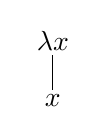
\begin{tikzpicture}[baseline=(root.base),level distance=5ex,inner ysep=0.5mm,sibling distance=10mm]
        \node (root) {$\lambda x$}child{node{$x$}};
    \end{tikzpicture}
    &
    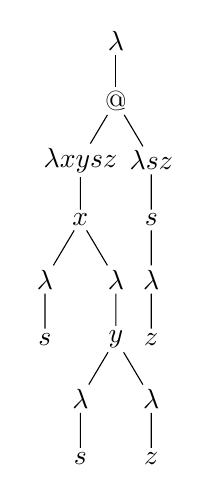
\begin{tikzpicture}[baseline=(root.base),level distance=5ex,inner ysep=0.5mm,sibling distance=9mm]
        \node (root)
        {$\lambda $}
        child {node{$@$}
            child{node{$\lambda x y s z$}
                child { node{$x$}
                    child{node{$\lambda $}{
                        child {node {$s$}}}
                    }
                    child{node{$\lambda $}
                        child{node{$y$}
                            child{node{$\lambda $}
                                child{ node {$s$}}
                            }
                            child{node{$\lambda $}
                                child{node{$z$}}}
                        }
                    }
                }
            }
            child{node{$\lambda s z$}
                child{node{$s$}
                    child{node{$\lambda $} child{node{$z$}}}
                }
            }
        };
    \end{tikzpicture}
    &
    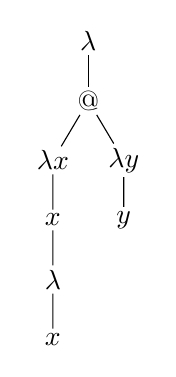
\begin{tikzpicture}[baseline=(root.base),level distance=5ex,inner ysep=0.5mm,sibling distance=9mm]
        \node (root)
        {$\lambda $}
        child {node{$@$}
            child{node{$\lambda x$}
                child { node{$x$}
                    child{node{$\lambda $}{
                        child {node {$x$}}}
                    }
                }
            }
            child{node{$\lambda y$} child{node{$y$}}}
        };
    \end{tikzpicture}
    &
    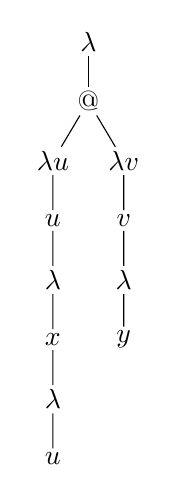
\begin{tikzpicture}[baseline=(root.north),level distance=5ex,inner ysep=0.5mm,sibling distance=9mm]
        \node (root)
        {$\lambda $}
        child {node{$@$}
                child{node{$\lambda u $}
                   child {node {$u$}
                      child {node {$\lambda $}
                          child {node {$x$}
                              child {node {$\lambda $}
                                  child {node {$u$}
                                  }
                              }
                          }
                      }
                   }
                }
                child{node{$\lambda v$}
                    child{node{$v$}
                        child{node{$\lambda $}
                            child{ node {$y$}}
                        }
                    }
                }
            };
        \end{tikzpicture}
    &
    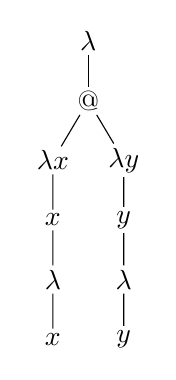
\begin{tikzpicture}[baseline=(root.base),level distance=5ex,inner ysep=0.5mm,sibling distance=9mm]
        \node (root)
        {$\lambda $}
        child {node{$@$}
            child{node{$\lambda x$}
                child { node{$x$}
                    child{node{$\lambda $}{
                        child {node {$x$}}}
                    }
                }
            }
            child{node{$\lambda y$}
                child { node{$y$}
                    child{node{$\lambda $}{
                        child {node {$y$}}}
                    }
                }
            }
        };
    \end{tikzpicture}
    \end{tabular}
\end{sgmlfig}
\caption{Examples of trees of untyped lambda terms.}\label{fig:comptree_examples}
\end{figure}

We define the \textbf{\emph{enabling relation}}\index{enabling relation}
$\enables $ on tree nodes $\Nodes $ as the relation mapping (i) each $\lambda
$-node to all the variable nodes that it binds; (ii) the root of the tree to
all the free variable nodes; (iii) variable and application node to each one
of their child nodes. We number child nodes starting from $0$ for @-nodes and
from $1$ for variable nodes, so that the $0$th child denotes the operator of
a redex, while other children represent operands of either an @-node or a
variable node. We write $n \enables _{k} \lambda \overline{x}$, for $k\geq
0$, to indicate that lambda node $\lambda \overline{x}$ is the $k$th child of
a variable or application node $n$; $\lambda \overline{x} \enables _{k} n$,
for $k\geq 1$, to indicate that the label of a bound variable node $n$ is the
$k$th variable name bound in $\lambda \overline{x}$--that is node $n$ is
labelled $x_{k}$; and if $r$ denotes the root of the tree then we take the
convention $r \enables _{k} z$ for any free variable node $z$, where $k$
denotes the free variable index of $z$ according to some predefined numbering
of free variables. We say that a node \textbf{\emph{hereditarily
enables}}\index{hereditarily enables} another node if the two nodes relate by
the transitive closure of $\enables $. A tree node is
\textbf{\emph{external}}\index{external} if it is hereditarily enabled by the
root or it is the root itself, otherwise it is
\textbf{\emph{internal}}\index{internal}. We write $\ExternalNodes $ for the
set of external nodes. We write $\InternalNodes $ to denote the set of
internal nodes, which are therefore @-nodes and nodes hereditarily enabled by
@-nodes. The \textbf{\emph{arity}}\index{arity} of a node $n$, written $|n|$,
is defined for a variable node as the number of immediate arguments
(\textit{i.e.}, children in the tree); for an application node, as the number
of operands (\textit{i.e.}, number of children of the $@$-node minus 1); for
a lambda node $\lambda x_{1} \cdots x_{k}$, $k\geq 0$, as the number of bound
variables $k$.

%s2.4 #&#
\subsection{Extensional tree}\label{sec2.4}

We extend the notion of term tree by augmenting the \textbf{\emph{structural
nodes}}\index{structural nodes} $\Nodes $ of $\ctree (M)$, which represent
tokens in the syntax representation of the lambda term, with two countable
sets of \textbf{\emph{ghost nodes}}\index{ghost nodes} representing
fictitious tokens: The \textbf{\emph{ghost lambda nodes}}\index{ghost lambda
nodes}  have a unique label $\ghostlmd $ and represent fictitious lambda
abstractions. The \textbf{\emph{ghost variable nodes}}\index{ghost variable
nodes} have a unique label $\ghostvar $ and represent fictitious nameless
variable nodes. We define them by simultaneously and recursively extending
the parent-child node relation and the enabling relation associated with the
term tree: for every (ghost) variable or @-node $n$ with parent (ghost)
lambda node $\nu $, and for all $k>|n|$, we introduce a new node $\ghostlmd $
as the $k$th-child of $n$, and a new node $\ghostvar $ as the unique child of
that ghost lambda node. We extend the enabling relation with $n \enables _{k}
\ghostlmd $ and $\nu \enables _{|\nu |+ k} \ghostvar $; where by convention
ghost nodes have arity $0$, and the arity of structural nodes remains
unchanged (\textit{i.e.}, given by their arity in the structural tree $\ctree
(M)$). This extended enabling relation induces a binding relation between
ghost variables and their (possibly ghost) lambda-binder, which lets us forgo
the notion of variables names in ghost nodes: we can thus use respectively
$\ghostlmd $ and $\ghostvar $ as a unique label for all ghost lambda and
variable nodes.

The infinite tree hereby defined is called the \textbf{\emph{extensional
tree}}\index{extensional tree} $\exttree (M)$ over labels $\mathcal{L} \cup
\{ \ghostlmd , \ghostvar \}$. Its nodes $\ExtendedNodes $ consists of
structural nodes $\Nodes $ plus all ghost variables $\ghostvar $ and lambda
nodes $\ghostlmd $ as defined above. We write $\ExtendedNodesLmd $ for the
subset of lambda nodes (structural $\NodesLmd $ or ghosts $\ghostlmd $) and
$\ExtendedNodesVar $ for variable nodes (structural $\NodesVar $ or ghosts
$\ghostvar $).

%s2.5 #&#
\subsection{Justified sequence of nodes}\label{sec:justseq}

A \textbf{\emph{justified sequence}}\index{justified sequence} is defined a
sequence of nodes in $\ExtendedNodes $ where every occurrence $n$ in the
sequence may have an associated link called `justification pointer' pointing
to some previous node occurrence $j$ in the sequence, called its `justifier',
with an associated \textbf{\emph{link label}}\index{link label} $l\geq 0$;
with the constraint that the justifier node $\enables $-enables the source
node with the corresponding label; that is $j \enables _{l} n$ must hold. The
\textbf{\emph{link distance}}\index{link distance} is the number of
occurrences separating $n$ from its justifier $j$ plus $1$, or $0$ if $n$ has
no justifier. We represent a justified sequence as a sequence of labelled
node occurrences with back-pointing arrows for justification pointers. For
example: $\ldots\ \raisebox{-2pt}{\includegraphics{12154i01}}$, which we read `$n$ points to
$j$', or `$n$ is justified by $j$' with link label $l$. For readability, we
sometimes indicate the link label in exponent of the justified occurrence
instead of above the pointer, or we even omit the justification pointers
altogether. By abuse of notation, we often represent occurrences in
justification sequences by their corresponding node labels so that for
instance $\ldots \lambda \overline{x} \cdot x \ldots $ refers to an
occurrence of a node in $\ExtendedNodesLmd $ labelled $\lambda \overline{x}$
followed by an occurrence of a node in $\NodesVar $ with label $x \in \VarSet
$. Note that the enabling relation is \emph{statically} induced by the term
whereas the concept of justification is defined on node \emph{occurrences},
that is within a specific justified sequence. The \textbf{\emph{set of
justified sequences}}\index{set of justified sequences} over $M$, denoted
$\justseqset (M)$, consists of all justified sequences over $\ExtendedNodes$.

Let $s$ denote a justified sequence. We write $s^\omega $ to denote the last
occurrence of $s$. For any occurrence $n$ in $s$ we write $s_{\leq n}$ for
the prefix of $s$ ending at $n$, and $s_{<n}$ for the prefix ending
immediately before $n$. We say that $s$
\textbf{\emph{extends}}\index{extends} $u$ if $u$ is a strict prefix of $s$.
A sequence $s$ is \textbf{\emph{maximal}}\index{maximal} in $T\subseteq
\justseqset (M)$ if there is no sequence in $T$ that extends it. For any set
$T\subseteq \justseqset (M)$ we write $T^{\max }$ for the subset of maximal
sequences of $T$. We borrow basic definitions from Game
Semantics~\cite{Abr02}. A justified sequence verifies the
\textbf{\emph{alternation condition}}\index{alternation condition} if it
starts with a lambda node and subsequently alternates between (i) a variable
or application node (ii) a lambda node. An occurrence in $s$ is
\textbf{\emph{hereditarily justified by some other
occurrence}}\index{hereditarily justified by some other occurrence} if
recursively following justification pointers starting from the first
occurrence leads to the second one. Since justification pointers honor the
enabling relation $\enables $, if an occurrence of node $n$ is hereditarily
justified by the occurrence of a node $m\in \Nodes $ then $n$ is necessarily
hereditarily enabled by $m$. Further, if $m$ occurs only once in $s$ then the
occurrences hereditarily justified by $m$ are precisely the occurrences of
nodes that are hereditarily \emph{enabled} by $m$ in $\ctree (M)$. The
\textbf{\emph{projection}}\index{projection} $s\upharpoonright  n$ of $s$
with respect to $n$ is the subsequence consisting of occurrences hereditarily
justified by $n$ in $s$. We write $s \upharpoonright  A$ for the subsequence
of $s$ consisting of occurrences of nodes in a subset $A \subseteq \Nodes $.
Hence $s\upharpoonright  \ExternalNodes $ consists of occurrences of $s$ that
are external nodes, or equivalently that are hereditarily justified by some
occurrence of the root in $s$.

The P-view is the sub-sequence obtained by reading a justified sequence
backwards and skipping occurrences lying under the justification pointer of a
lambda node:

%d2.2 #&#
\begin{definition}\label{def:views}
The \textbf{\emph{P-view $\ulcorner  s \urcorner  $}}\index{P-view $\ulcorner
s \urcorner  $} of a justified sequence $s$ is defined recursively by:
$\ulcorner  \epsilon   \urcorner   = \epsilon $, $\ulcorner  s \cdot  n
\urcorner   =  \ulcorner  s \urcorner   \cdot n$ if $n$ is a variable or $@$
node; $\raisebox{-1pt}{\includegraphics{12154i02}}$ if $n$ is a lambda node; and  $\ulcorner
s \cdot  n  \urcorner    =  n$ if $n$ is a lambda node with no pointer. The
dual notion $\llcorner  s \lrcorner  $ of
\textbf{\emph{O-view}}\index{O-view} is given by $\llcorner  \epsilon
\lrcorner   = \epsilon $; $\llcorner  s \cdot  n  \lrcorner    =  \llcorner
s \lrcorner   \cdot n$ for $\lambda $-node $n$; $\raisebox{-1pt}{\includegraphics{12154i03}}$
for variable node $x$; and $\llcorner  s \cdot  @  \lrcorner   = @$. Given
two occurrences $n$ and $m$ in a justified sequence $s$, we say that $n$ is
\textbf{\emph{visible at}}\index{visible at} $m$ just if $n$ occurs in the
P-view $\ulcorner  s_{\leq  m} \urcorner  $.
\end{definition}

%s2.6 #&#
\subsection{Name-free and name-preserving encoding}\label{sec2.6}

The \textbf{\emph{(name-free) structure}}\index{(name-free) structure} of a
justified sequence is obtained by discarding node labels while preserving
node types, arities and justification pointers. It is encoded as a sequence
of elements from $(\mathbb {N}\times \mathbb {N}\times \mathbb {N}) +
(\mathbb {N}\times \mathbb {N}) + \{ @ \}$ where $(a, j, i)$ represents a
lambda occurrence of arity $a$ with link distance $j$ and link label $i$ ($0$
for no pointer); $(j, i)$ represents a variable occurrence with link distance
$j$ and link label $i$; and $@$ represents the occurrence of an application
node. Two sequences $s$ and $u$ over possibly two distinct terms are
\textbf{\emph{equivalent}}\index{equivalent}, written $s \equiv u$ just if
they have the same structure: the type (variable, @-node or $\lambda $-node),
arity, link distance and link label of the underlying occurrences match
pairwise. Two equivalent sequences are not necessarily equal since they may
have different variable names. Two subsets $J_{1}\subseteq \justseqset
(M_{1})$ and $J_{2}\subseteq \justseqset (M_{2})$ are
\textbf{\emph{isomorphic}}\index{isomorphic}, written $J_{1}\structisomorphic
J_{2}$, if  there exists a structure-preserving bijection between $J_{1}$ and
$J_{2}$; that is a bijection $\phi :J_{1}\longrightarrow J_{2}$ such that
$s\equiv \phi (s)$ for all $s\in J$.

%e2.1 #&#
\begin{example}
Alpha-conversion preserves the structure so for instance we have
$\raisebox{-1pt}{\includegraphics{12154i04}}$.
\end{example}

The \textbf{\emph{name-preserving encoding}}\index{name-preserving encoding}
of a justified sequence of nodes with variables in $\VarSet $ is a sequence
of elements in $\nameencoding = (\mathcal{V}^{*}\times \mathbb {N}\times
\mathbb {N}) + (\mathbb {N}\times \mathbb {N}) + \{ @ \}$  defined
occurrence-wise similarly to the name-free encoding except for lambda nodes
where an occurrence $\lambda \overline{x}\in \ExtendedNodesLmd $ with link
distance $j$ and link label $i$ gets encoded as $(\overline{x},j,i) \in
\mathcal{E}$. The \emph{readout function} $\readout : \nameencoding ^{*}
\rightarrow \mathcal{L}^{*}$ decodes a name-preserving encoding into a
sequence of node labels in $\mathcal{L}$, and is given by $\readout [\epsilon
]= \epsilon $; $\readout [s \cdot @] = \readout [s] \cdot @$; $\readout [s
\cdot (\overline{x}, j, i) ] = \readout [s] \cdot \lambda \overline{x}$ and
for any encoding $s = u \cdot (\overline{x}, k, l)\,  n_{1} \ldots n_{j-1}$
where $u \in \nameencoding ^{*}$, $n_{1}, \ldots n_{j-1}\in \nameencoding $,
$j\geq 1$, $k,l\geq 0$, $\readout [s\cdot (j,i)] = \readout [s] \cdot x_{i}$
if $i\leq |\overline{x}|$, and $\readout [s\cdot (j,i)]  = \readout [s] \cdot
\ghostvar $ if $i> |\overline{x}|$. Just like the name-free encoding, this
encoding assimilates the ghost lambda `$\ghostlmd $' with the dummy lambda
`$\lambda $', so that the case $\lambda \overline{x}$ where
$\overline{x}=\epsilon $ covers both the ghost lambda and dummy lambda. We
then define $\readout \colon \nameencoding ^{*} \rightarrow \mathcal{L}^{*}$
by point-wise extension.

%e2.2 #&#
\begin{example}\label{examp:ghost_materialization}
Take the term $M = \lambda x. (\lambda y z.z) u$. The nodes of the
extensional tree $\exttree (M)$ are $\ExtendedNodes = \{ \lambda x, @,
\lambda y z, z, \lambda , u \} + \ghostvar + \ghostlmd $. The justified
sequence $t = \raisebox{-2pt}{\includegraphics{12154i05}} $ has name-preserving encoding $(x
,0,0)\cdot @\cdot (y\, z, 1,0)\cdot (1,2)\cdot (\epsilon ,3,2)\cdot (5,2)$,
whereas the sequence encoding $ (x\, g, 0, 0)\cdot @\cdot (y\, z\, x\, y\, y,
1,0)\cdot (1,2)\cdot (\epsilon ,3,2) \cdot (5,2)$ encodes the justified
sequence $s= \raisebox{-2pt}{\includegraphics{12154i06}} $ which reads out as $\readout [s]=
\lambda x g \cdot @ \cdot \lambda y z x y y \cdot z \cdot \lambda \cdot g$.
\end{example}

The main results of the paper apply to both encodings, though the
name-preserving presentation has the advantage of reusing names from the
original terms when producing the normal form. We thus adopt that encoding in
the rest of the paper and take $\justseqset (M)$ to be a (strict) subset of
$\nameencoding ^{*}$.

%s2.7 #&#
\subsection{Justified paths of the term tree}\label{sec2.7}

We define the \textbf{\emph{set of justified paths}}\index{set of justified
paths} $\pathset (M)$ of a term $M$ as the set of justified sequences in
$\justseqset (M)$ whose underlying sequences of nodes are those from the
paths of the labelled-tree $\ctree (M)$ and justification pointers are
induced by the enabling relation: bound variable nodes point to their binder
$\lambda $-node, which necessarily occurs in the path to the root, with link
label set to the index of the variable name in the binding $\lambda $-node;
free variables point to the initial occurrence (the tree root) with link
label  set to an index in $\mathbb {N}$ uniquely identifying the free
variable name; and lambda nodes are justified by the immediate predecessor in
the path sequence, which is also its parent node by definition of a tree
path, with label index given by its child index.

%p2.1 #&#
\begin{property}[Path characterization]\label{prop:tree_path_charact}
An untyped term $M$ is uniquely determined (i) by the maximal justified paths
of $\pathset (M)$; or (ii) up to $\alpha $-conversion, by the
\emph{structure} of the maximal justified paths of $\pathset (M)$.
\end{property}

\begin{proof}
(i) A $\lambda $-term $M$ is uniquely determined by its term tree $\ctree
(M)$, itself uniquely determined by its maximal paths, which can be
reconstructed from the justified maximal paths (labels are the same, and the
child index is $1$ for variable/@ nodes and is given by the justification
label for lambda nodes). (ii) Variables bindings are uniquely determined by
the justification pointers with their associated label; so maximal justified
paths are  reconstructible from their structure, up to $\alpha $-conversion,
by assigning fresh variable names to all lambda nodes.
\end{proof}

%e2.3 #&#
\begin{example}
The maximal justified paths of $\pathset ((\lambda x.x y) (\lambda z.z))$ are
$\{\raisebox{-1pt}{\includegraphics{12154i07}},\raisebox{-1pt}{\includegraphics{12154i08}}\}$.
\end{example}

A set of name-preserving justified sequences $T\subset \nameencoding ^{*}$ is
\textbf{\emph{$\alpha  $-consistent}}\index{$\alpha  $-consistent} if all its
`path-like' justified sequences agree on how to name bound-variables in
lambda nodes: if $p \cdot (\overline{x}, 1, i)$ and $p \cdot (\overline{y},
1, i)$ are in $T$ for $i\geq 0$, $p\in \nameencoding ^{*}$ then $\overline{x}
= \overline{y}$.

%p2.2 #&#
\begin{proposition}[Term read-out]\label{proposition:termtree_readout_from_justitied_paths}
Let $T\subset \nameencoding ^{*}$ be a finite $\alpha $-consistent set of
(name-preserving encoded) justified sequences. If $T\structisomorphic
\pathset (M)$ for some (a priori unknown) untyped term $M$ then one can
effectively construct an untyped term  $\readout [T]$ that is $\alpha
$-equivalent to $M$, and which preserves variables names as defined by the
$\lambda $-binders in $T$, except where a variable capture situation occurs.
\end{proposition}

\begin{proof}
Because $T \structisomorphic \pathset (M)$, the sequences in $T$ have the
properties of justified paths of a term tree: they start with a lambda,
alternate between lambda and variable/@, contain no ghost nodes, lambdas have
a single child and are justified by their immediate predecessor in the
sequence (their parent). Furthermore, $T$ induces an arity for each
occurrence of a sequence in $T$: the arity of a lambda-occurrence
$(\overline{x},j,i)\in \nameencoding $ is $|\overline{x}|$, the arity of a
variable or @-occurrence is the maximum child-index (given by the link label)
of any lambda occurrence immediately following it in any sequence of $T$.
This allows us to construct a $\mathcal{L}$-labelled tree inductively from
the maximal sequences of $T$. We first inductively construct a
$\mathcal{L^{-}}$-labelled tree with $\mathcal{L^{-}} = \{ @ \} + \{ \lambda
\overline{x} \ | \ \overline{x} \in \mathcal{V}^{*} \} + \mathbb {N}\times
\mathbb {N}$, where a De Bruijn pair $(j,i)\in \mathbb {N}\times \mathbb {N}$
represents a variable node such that the link distance $j$ identifies the
binder lambda node, and the link label $i$ gives the bound variable index in
that binding lambda node. Since $T$ is $\alpha $-consistent, there is a
single choice of variable names $\overline{x}$ to assign to a given lambda
node.

An important step at this point is to rename variables to avoid any potential
variable capture when we finally replace the De Bruijn pairs by the variable
names they refer to. Firstly, the variable names $\overline{x}$ from
lambda-occurrences in sequences in $T$ may contain duplicates. We resolve
this by renaming names that are repeated within the same lambda node,
provided that some variable occurrence under that node refers to the first
variable name: this is the situation of a justified path  $\cdots \lambda x x
y \cdots (j,1)$ where the De Bruijn pair $(j,1)$ refers to the first $x$ of
the lambda node. In this case, the lambda node becomes $\lambda x x' y$.
Secondly, two distinct nested lambdas in a given justified path may bind the
same variable name. If this introduces a clash, \textit{i.e.}, the variable
occurs freely under the nested lambda, then we rename the bound variable in
the nested lambda. This is the situation of a justified path of the form
$\cdots \lambda{xyz} \cdots \lambda {xuv} \cdots (j,1) \cdots $ where the De
Bruijn pair $(j,1)$ refers to the $x$ from the first lambda $\lambda{x y z}$.
After renaming variables in the $\mathcal{L^{-}}$-labelled tree, we obtain
the final $\mathcal{L}$-labelled tree by replacing all De Bruijn pairs
$(j,i)$ with the $i$th variable name from the lambda node located $j$ nodes
above it in the term tree, as implemented by the name-preserving readout
function $\readout [\_]$ on justified sequences. Interpreting that
$\mathcal{L}$-labelled as a term tree $\ctree (\_ )$ lets us read back from
it the underlying untyped term $N$. By construction we have $\pathset (N) =
T$ therefore $N$ and $M$ have the same justified paths structures so by
\reftext{Property~\ref{prop:tree_path_charact}} they must be $\alpha
$-equivalent.
\end{proof}


%s3 #&#
\section{Imaginary traversals}\label{sec:imaginary_traversals}

%s3.1 #&#
\subsection{Definition and properties}

%d3.1 #&#
\begin{definition}
The set $\travulc (M)$ of \textbf{\emph{traversals}}\index{traversals} of an
untyped lambda term $M$, abbreviated $\travulc $ when the term is clear from
context, is the set of justified sequences of nodes over the extensional tree
of $M$, defined inductively by the derivation rules of
\reftext{Table~\ref{tab:trav_rules}}: We have $t \in \travulc (M)$ if and
only if the judgment $\istraversal t$ is derivable. We use interchangeably
`\emph{imaginary traversal}' or just `\emph{traversal}' when referring to a
traversal of an untyped term.
\end{definition}

%t1 #&#
\begin{table}[t]
\caption{Derivation rules of imaginary traversals $\travulc $ of the untyped $\lambda $-calculus.}
\label{tab:trav_rules}
\includegraphics{12154i10}
%\begin{sgmlfig}
%\begin{ruletablebox}{} \noindent \textbf{PROGRAM -- Structural rules}
%\begin{itemize}[leftmargin=3em]
%    \item[$\mathsf{(Root)}$]
%    $\istraversal \nu $ if $\nu $ is the root $\lambda $-node of the term tree $\ctree (M)$.
%
%    \item[$\mathsf{(App)}$] If $\istraversal t \cdot @$ then
%    $\istraversal \Pstr[0.4cm]{t \cdot (at) @  \, (a-at,40:0) \nu }$ where $\nu \in \NodesLmd $ is the $0$th child $\lambda $-node of $@$.
%
%    \item[$\mathsf{(Lam)}$] If $\istraversal t \cdot \nu $ for $\nu \in \ExtendedNodesLmd $ then $\istraversal t \cdot \nu ~ n$ where $n$ is $\nu $'s unique child and if $n$ is
%    \begin{compactitem}
%        \item[$\mathsf{(Lam^{@})}$] an $@$-node then it has no justifier;
%        \item[$\mathsf{(Lam^{\mathsf{var}})}$] in $\NodesVar $ then it points to the only occurrence in $\ulcorner  t\cdot  \nu   \urcorner  $ of a node $m$ verifying $m \enables _{k} n$ for some $k\geq 0$, and has link label $k$;
%
%        \item[$\mathsf{(Lam^{\ghostvar}  )}$] a ghost variable $\ghostvar $
%        (thus $\nu $ is $\ghostlmd $) then
%        it points to the predecessor $\mu $ of $\nu $'s justifier $m$, and has link label $|\mu | + i - |m|$
%        where $i$ is the link label of $\nu $. That is
%        $\istraversal \Pstr[0.5cm]{ u \cdot (alphaprime){\mu }\, (m){m} \cdot v \cdot  (gl-m,30:i){\ghostlmd }\, (al-alphaprime,43:{|\mu | + i - |m|}){\ghostvar }}$
%    where
%        $t \cdot \nu = \Pstr[0.5cm]{ u \cdot
%        \mu \, (m){m} \cdot v \cdot (gl-m,40:i){\ghostlmd }}$,
%        $\mu  \in \ExtendedNodesLmd , m \in \ExtendedNodesVar \cup  \NodesApp $.
%    \end{compactitem}
%\end{itemize}
%\emph{\textup{\textbf{PROGRAM -- Copy-cat rule}}}
%\begin{itemize}[leftmargin=3em]
%\item[$\mathsf{(Var)}$] If $\istraversal \Pstr[0.5cm]{t\cdot (m){m}
% \, (alphaprime){\mu }
%\cdot v \cdot (n-alphaprime,50:i){n}}$ for $m \in \ExtendedNodesVar \cup  \NodesApp $, $\mu \in \ExtendedNodesLmd \cap  \InternalNodes $, $n \in \ExtendedNodesVar \cap  \InternalNodes $, $i>0$ then
%  $\istraversal \Pstr[0.3cm]{ t  \cdot
%(m){m}\, (lx){\mu }  \cdot v \cdot (x-lx,30:i){n}
%    \, (letai-m,45:i){\nu }}$
%    where $\nu $ denotes the $i$th child ($\lambda $-node) of $m$.
%\end{itemize}
%
%\emph{\textup{\textbf{DATA -- Input-variable rule}}}
%\begin{itemize}[leftmargin=3em]
%\item[$\mathsf{(IVar)}$] If $\istraversal t \cdot n$ with $n \in \ExtendedNodesVar \cap  \ExternalNodes $ then
%for every $i$th child $\nu $ of any node $m \in \ExtendedNodesVar $ occurring in $\llcorner  t\cdot  n \lrcorner  $, $i\geq 1$, we have
%$\istraversal t \cdot n ~ \nu $ where $\nu $ points to $m$ with label $i$.
%\end{itemize}
%
%where $t, u,v$ denote sub-sequences of justified sequences of nodes.
%\end{ruletablebox}
%\end{sgmlfig}
\end{table}




%e3.1 #&#
\begin{example}\label{ex:ulctrav_sample}
Take the term $J = (\lambda u . u(x\,u)) (\lambda v . v\,y)$, whose tree is
represented in \reftext{Fig.~\ref{fig:comptree_examples}}. We have the
traversal $t = \raisebox{-2pt}{\includegraphics{12154i09}} \in \mathcal {T}\!rav(J)$ where
each justification label is indicated in exponent of the corresponding
justified occurrence.
\end{example}

%p3.1 #&#
\begin{proposition}\label{prop:ulctrav_welldefined_pathview}
The traversal rules are well-defined, in particular for any sequence of nodes
with pointers $t\in \mathcal {T}\!rav$ we have:
%c3.1 #&#
%
\begin{enumerate}[\textit{(iii)}]
\item[\textit{(i)}] $t$ is a valid justified sequence, with respect to the enabling
    relation $\enables $ on $\ExtendedNodes $, and verifies the alternation
    condition;
\item[\textit{(ii)}] For all occurrences ${\includegraphics{12154i11}}$, $n$ is a
    ghost node if and only if $i > |m|$;
\item[\textit{(iii)}] $\ulcorner  t \urcorner  $ is a (justified) path in the
    extensional tree $\exttree (M)$; So if $t$ does not contain ghost nodes
    then $\ulcorner  t \urcorner  $ is a structural path in $\ctree (M)$.
\end{enumerate}
\end{proposition}

\begin{proof}
Proven simultaneously by induction on the traversal rules. For
$\mathsf{(Lam^{\mathsf{var}})}$: By induction hypothesis (iii) the P-view is
a path in the extensional tree of $M$. But the last node of $t$ is a
structural node therefore, this path is necessarily a structural path with no
ghost node. Consequently, if the last node is a bound variable node, its
enabler is precisely its binding lambda node which necessarily occurs exactly
once in the path to the root. If the variable is free then the enabler is the
root itself and (i) holds. By definition, the justification pointer honors
the enabling relation so (ii) holds. The node $n$ is by definition the unique
child of $\nu $ thus (iii) holds. For $\mathsf{(Lam^{\ghostvar}  )}$, the
induction hypothesis (ii) shows that $i>|m|$, which guarantees that $|\mu
|+i-|m|>0$ is a valid justification label (i) and that (ii) holds for the
traversed ghost node $\ghostvar $. Finally (iii) holds because the node
preceding $\ghostvar $ in the P-view is precisely $\mu $, its parent node.
Other rules are straightforward.

Observe that by (iii), the P-view at a given occurrence uniquely determines
the corresponding tree node. This allows us to look up child/parent nodes
when applying traversal rules, even with an underlying sequence encoding,
such as $\mathcal{E}^{*}$, that omits tree structure information.
\end{proof}

The last property generalizes a concept from the theory of
traversals~\cite{OngLics2006,BlumPhd} to the untyped setting: The
game-semantic concept of P-views corresponds to paths in the computation
tree.

%p3.1 #&#
\paragraph*{On-the-fly eta-expansion}
The rules $\mathsf{(Var)}$ and $\mathsf{(IVar)}$ are responsible for
performing the `on-the-fly eta-expansion'. If the arity of the traversed
variable is sufficiently high, the tree statically dictates the structural
node to traverse next--we have $i \leq |m|$ and $\nu $ is a structural lambda
node in $\NodesLmd $; we call this the \textbf{\emph{concrete
sub-case}}\index{concrete sub-case}. Otherwise, the variable arity is too low
to statically determine the requested operand of the application--we have $i
> |m|$ and $\nu $ is a ghost lambda node $\ghostlmd $; we call this the
\textbf{\emph{imaginary sub-case}}\index{imaginary sub-case}.

%d3.2 #&#
\begin{definition}
{\textbf{\emph{Ghost materialization}}}\index{Ghost materialization} refers
to the instantiation of a traversal rule where the last occurrence prior to
applying the rule is a ghost and the node traversed is structural. Inspection
of the traversal rules shows that this may only happen in rule
$\mathsf{(Var)}$, so that once a traversal starts traversing ghost nodes, the
only way to `return' to structural nodes is via $\mathsf{(Var)}$ with a
traversal of the form $\raisebox{-2pt}{\includegraphics{12154i12}}$ where $\lambda
\overline{x} \in \NodesLmd $ is the $i$th child lambda node of some
structural variable node $y \in \NodesVar $, and $\nu $ is a $\lambda $-node
verifying $0\leq |\nu | < i \leq |y|$.
\end{definition}

Rule $\mathsf{(Lam)}$ traverses a lambda node by just visiting its unique
child  in the tree, which is necessarily a structural node. Its counterpart
$\mathsf{(Lam^{\ghostvar}  )}$ traverses a ghost lambda by visiting the
imaginary ghost variable that would be created if we were to eta-expand the
sub-term under that lambda: the ghost placeholder $\ghostvar $ represents an
occurrence of the $j$th variable bound by lambda node $\mu $ if the sub-term
at node $\mu $ were eta-expanded $i-|n|$ times; hence $j = |\mu | + i - |m|$.
Observe that we necessarily have $i>|n|$ since the $i$th child of $n$ is a
ghost variable node.

The successive fictitious eta-expansions of $M$ can be reconstructed from the
traversal itself:

%d3.3 #&#
\begin{definition}\label{def:onthefly_etaexpansion}
Let $M$ be an untyped term and $n\in \Nodes $ be the root node of some
subterm $N$. We define $\mathsf{ETA}(M, n, k)$ as $M$ if $k \leq 0$ ; and for
$k> 0$ as the term obtained from $M$ by substituting in-place $N$ with
$\lambda z_{1} \cdots z_{k}. N z_{1} \cdots z_{k}$ for some variables $z_{1},
\ldots , z_{k}$ fresh in $N$. We define inductively $M^{t}$,  the
\textbf{\emph{eta-expansion of $M$ with respect to a finite traversal
$t$}}\index{eta-expansion of $M$ with respect to a finite traversal $t$}, by
$M^\epsilon = M$, $M^{u \cdot n} = M$ if $n$ has no justifier, and if $m$
denotes $n$'s justifier in $u$ with link label $i$ then $M^{u \cdot n} =
\mathsf{ETA}(M^{u}, m, i-|m|)$. (Note that $i>|m|$ holds only for the
imaginary sub-case of $\mathsf{(Var)}$ and $\mathsf{(IVar)}$.)
\end{definition}

%e3.2 #&#
\begin{example}
The eta-expansion of $J = (\lambda u . u(x\,u)) (\lambda v . v\,y)$ with
respect to traversal $t$ from \reftext{Example~\ref{ex:ulctrav_sample}} is
$J^{t} = (\lambda u . u(x (\lambda z_{1}. u (\lambda z_{2}.z_{1}\,z_{2}))))
(\lambda v . v\,y)$ for some fresh variable names $z_{1}, z_{2}$.
\end{example}


%p3.2 #&#
\begin{proposition}\label{prop:eta_expanded_trav}
Let $M$ be an untyped term and $t$ be a \emph{finite} traversal of $M$. There
exists a one-to-one function $\eta _{t} : \ExtendedNodes (M) \longrightarrow
\ExtendedNodes (M^{t})$ such that its implicit \emph{element-wise
pointer-preserving} extension $\eta _{t} : \mathcal{J}(M) \longrightarrow
\mathcal{J}(M^{t})$ verifies the properties:
%
\begin{enumerate}[\textit{(iii)}]
\item[\textit{(i)}] If $u \in \travulc (M)$ then $\eta _{t}(u) \in \travulc
    (M^{t})$, and thus $\ulcorner  \eta  _{t}(u) \urcorner  $ is a
    \emph{structural} path in $\ctree (M^{t})$.

\item[\textit{(ii)}] If $v \in \travulc (M^{t})$ then there exists a traversal $u\in
    \travulc (M)$ such that $v = \eta _{t}(u)$.

\item[\textit{(iii)}] The restriction of $\eta _{t}$ to $\mathcal {T}\!rav(M)$
    defines a structure-preserving bijection with $\mathcal
    {T}\!rav(M^{t})$.
\end{enumerate}
\end{proposition}

\begin{proof}
The tree $\ctree (M)$ being by definition a subtree of $\ctree (M^{t})$,
induces a one-to-one mapping $\eta _{t}$ from $\Nodes (M)$ to $\Nodes
(M^{t})$ which we extend point-wise to justified sequences. We show (i) by
induction on $u$ observing that in the imaginary sub-case, the rules
$\mathsf{(Var)}$ and $\mathsf{(IVar)}$ increase the arity of the justifier
node $m$, which guarantees that the corresponding structural node exists in
$\ctree (M^{t})$. (ii) is shown similarly by induction on $v$. (iii) follows
from (i) and (ii).
\end{proof}

%\proofatend
%The tree $\ctree (M)$ being by definition a subtree of $\ctree (M^t)$, induces a one-to-one mapping from $\Nodes (M)$ to $\Nodes (M^t)$.
%We extend it to ghost nodes by mapping ghost occurrences in $t$ to the corresponding node resulting from the eta-expansions of subterms of $M$ in $M^t$, and all other ghost nodes not occurring in $t$ to the corresponding ghost nodes in $\ctree (M^t)$. Formally, we define $\eta _t$ by induction on the traversal $t$, observing that the eta-expansion performed in rules \rulenamet{Var} and \rulenamet{IVar} in Definition~\ref{def:onthefly_etaexpansion} increases the arity of the justifier node $m$, which guarantees that the corresponding structural node exists in $\ctree (M^t)$.
%
%(i) By induction on $u$. Reusing the rule used to traverse $u$ to traverse $\eta _t(u)$. For \rulenamet{Var} and \rulenamet{IVar}, in the \emph{imaginary} sub-case, if the ghost variable traversed also appears in $t$ then we use instead the \emph{concrete} sub-case of the corresponding rule to traverse $\eta _t(u)$.
%
%(ii) By induction on $v$, applying to $u$ each rule that is applied to $v$. For the case \rulenamet{Var} and \rulenamet{IVar}, if the index $i$ is greater than the arity of the node $m$ in $M$ then the lambda node from $v$ gets replaced by a ghost lambda node in $u$.
%
%(iii) By (i) the function is well-defined, it is injective by definition, and by (ii) it is surjective.
%\endproofatend
%
%e3.3 #&#
\begin{example}
Continuing with \reftext{Example~\ref{ex:ulctrav_sample}},
the traversal $t$ of $J$ corresponds to the
traversal\\
$\raisebox{-2pt}{\includegraphics{12154i13}}$ of $J^{t}$ where nodes resulting from the
eta-expansions are underlined.
\end{example}

%d3.4 #&#
\begin{definition}\label{ref:strand}
A \textbf{\emph{strand}}\index{strand} of a traversal, is a sub-sequence of
consecutive occurrences of even length, starting with an external lambda node
and ending with an external variable node, with only internal node
occurrences in-between.

From the parity property of traversals, a strand must consist of alternations
of lambda nodes and variable/application nodes. To highlight a strand within
a traversal we sometimes underline its opening and closing occurrence as
follows: $ t = \cdots \underline{\nu _{k}}\ n_{k}\ \nu _{k-1}\ n_{k-1}\
\cdots \ \nu _{2}\ n_{2}\ \nu _{1}\ \underline{n_{1}} \cdots $ for some
$k\geq 1$ where for $1 \leq j \leq k$, $\nu _{j}$ is in $\ExtendedNodesLmd $,
$n_{j}$ is in $\ExtendedNodesVar \cup  \NodesApp $, the external lambda $\nu
_{k}$ and external variable $n_{1}$ delimit the strand boundaries and the
$2k-2$ nodes in-between are all internal.
\end{definition}

We say that a traversal has \textbf{\emph{complete strands}}\index{complete
strands} if every external lambda occurrence is eventually followed by an
occurrence of an external variable. Otherwise, we say that the last strand in
the traversal is \emph{incomplete}. A finite \emph{maximal} traversal has
necessarily complete strands, for if it were not ending with an external
variable we could extend it with either $\mathsf{(App)}$, $\mathsf{(Lmd)}$ or
$\mathsf{(Var)}$.

%p3.1 #&#
\paragraph*{Traversal core}
In the typed setting, the \emph{core of a traversal}~\cite{BlumPhd} is simply
obtained by removing all internal occurrences from a traversal. Generalizing
this notion to the untyped setting requires additional relabelling of lambda
nodes.

We consider sequences in $\VarSet ^{*}$ as stacks of variable names equipped
with  push and pop operations: for any stack $\overline{x} = x_{1} \ldots
x_{n}$, $n,j\geq 0$, $pop_{j} (x_{1} \ldots x_{n}) = x_{j+1} \ldots x_{n}$ if
$j<n$, and $pop_{j} (x_{1} \ldots x_{n}) = \epsilon $ otherwise; pushing
elements onto the stack is done via sequence concatenation: pushing  variable
names $\overline{x}$ onto stack $\overline{y}$ yields  $\overline{x} \cdot
\overline{y}$.

%d3.5 #&#
\begin{definition}[Core projection]\label{def:coreprojection}
Let $\overline{y} \in \VarSet ^{*}$ denote a stack of variable names. We
define the partial function $\coresymbol _{\overline{y}}\colon \justseqset
(M) \longrightarrow \justseqset (M)$ on finite justified sequences by
induction: $\coresymbol _{\overline{y}}(\epsilon ) = \epsilon $, and for any
justified sequence $s \cdot n\in \justseqset (M)$ with prefix $s \in
\justseqset (M)$ and node occurrence $n\in \ExtendedNodes $:
%
\begin{equation*}
\coresymbol _{\overline{y}}(s\cdot n) =
\begin{cases}
\coresymbol _{\epsilon }(s) \cdot n    & \mbox{if } n\in \ExtendedNodesVar \cap  \ExternalNodes , \\
\coresymbol _{pop_{|n|}(\overline{y})}(s)    & \mbox{if } n\in (\ExtendedNodesVar \cap  \InternalNodes )\cup  \NodesApp , \\
\coresymbol _{\epsilon }(s) \cdot \lambda \overline{z}    & \mbox{if $n  \in \ExtendedNodesLmd \cap  \ExternalNodes $,
$n$ is labelled $\lambda \overline{x}$ and $\overline{z}=\overline{x}\cdot \overline{y}$,} \\
\coresymbol _{\overline{x} \cdot \overline{y}}(s)    & \mbox{if $n \in \ExtendedNodesLmd \cap  \InternalNodes $ and $n$ is labelled $\lambda \overline{x}$,}
\end{cases}
\end{equation*}
%
where the justification pointers from the left-side of the equality are
preserved--that is the link distance of each occurrence is adjusted for the
occurrences removed between it and its justifier. This is well-defined since
an external node can only be justified by another external node. Note that
the last two equalities handle the ghost lambda case when
$\overline{x}=\epsilon $. We define the \textbf{\emph{core}}\index{core} of
justified sequence $s$ as $\coresymbol _\epsilon (s)$, abbreviated
$\core{s}$, and its \textbf{\emph{core P-view}}\index{core P-view} as
$\ulcorner  \core {s} \urcorner  $--the P-view of its core.
\end{definition}

The subscript parameter in `$\coresymbol _{\overline{y}}$' is called
\textbf{\emph{stack of pending lambdas}}\index{stack of pending lambdas}. As
$\coresymbol $ reads a strand backwards, it accumulates variable names which
then get discharged onto the opening lambda node of the strand. This
definition has a name-free counterpart that uses a stack length argument in
place of the stack argument $\overline{y}$. We sometimes indicate the pending
lambdas in exponent of external lambda nodes as follows: $\cdots  \lambda
\overline{x}^{[\overline{y}]} \cdots $, where $\overline{y}$ denotes the
pending lambdas at $\lambda \overline{x}$, to hint on how the traversal core
is calculated.

Some immediate properties follow: (i) The core of a justified sequence
contains external nodes only therefore $\coresymbol $ is idempotent. (ii) If
$M$ is in beta-normal form then all the nodes of $\exttree (M)$ are external;
thus the core projection coincides with the identity. (iii) When discharging
new variable names onto a lambda node, core projection can cause variable
name reuse, but the justification pointers from the underlying name-free
structure prevent any possible ambiguity.

%e3.4 #&#
\begin{example}
The traversal $t = \lambda w^{[y]} ~ @ ~ \lambda x y ~ x ~ \lambda ~ z$ of
$\lambda w . (\lambda x y .x) z$ has core $\coresymbol (t) = \lambda w y ~
z$.
\end{example}


%e3.5 #&#
\begin{example}
Take $(\lambda x. x x)(\lambda y. y)$ with traversal $t$ represented below.
Projecting external nodes gives $t\upharpoonright  \ExternalNodes =
\raisebox{-2pt}{\includegraphics{12154i14}}$ whereas the core projection gives $\coresymbol
(t) = \raisebox{-2pt}{\includegraphics{12154i15}}$.
%
\begin{eqnarray*}
t = \includegraphics{12154i16}
\end{eqnarray*}
\end{example}



%s3.2 #&#
\subsection{Eta-long traversals of simply-typed terms}\label{sec3.2}

A notable limitation of the traversals for simply-typed languages, such as
STLC and PCF~\cite{BlumPhd}, is that the \textbf{\emph{eta-long
form}}\index{eta-long form} of the term is traversed rather than the term
itself. This transformation ensures that every strict subterm that is not of
atomic type  necessarily has another term applied to it. The formal
definition~\cite{huet75-unification,BlumPhd,OngLics2006} is not essential so
we omit it here. In practice, it means that the term tree gets transformed by
eta-expanding all variable and application nodes according to the type of the
subterm at that node: if the type is $\tau _{1} \rightarrow \ldots (\tau _{m}
\rightarrow o)$ and the node has $n$ children with $n< m$ then the subterm is
eta-expanded $m-n$ times. In the \emph{simply-typed} lambda calculus,
variable names in the lambda nodes labels are \emph{typed-annotated}, but
those annotations are not used in any way by the STLC traversals rules. In
fact, if we erase all the type annotations, we can apply the rules of
imaginary traversals from \reftext{Table~\ref{tab:trav_rules}} on a
typed-term, and we observe that the definition of traversals from the typed
settings~\cite{BlumPhd} coincides with the rules of imaginary traversals that
do not involve ghost nodes:

%d3.6 #&#
\begin{definition}\label{def:concrete_traversals}
A \textbf{\emph{concrete traversal}}\index{concrete traversal} is an
imaginary traversal that does not contain any ghost occurrence. The set
$\mathcal {T}\!rav_{\concrete} $ of \textbf{\emph{concrete
traversals}}\index{concrete traversals} is defined by the rules of
\reftext{Table~\ref{tab:trav_rules}} with the exclusion of
$\mathsf{(Lam^{\ghostvar}  )}$ and by restricting rules $\mathsf{(Var)}$ and
$\mathsf{(IVar)}$ to their concrete sub-case where the traversed node must be
structural (\textit{i.e.}, $i\leq |m|$).
\end{definition}

We consider a typed-term $M^\tau $ of simple type $\tau $ that, without loss
of generality and to simplify notations, we assume to be closed (no free
variable).

%d3.7 #&#
\begin{definition}[Reformulation of~\cite{BlumPhd}]
The \textbf{\emph{eta-long traversals}}\index{eta-long traversals} of a
simply-typed term $M^\tau $ are $\mathcal {T}\!rav_{\concrete }(N^\tau )$,
the concrete traversals of its eta-long form $N^\tau $.
\end{definition}

%p3.3 #&#
\begin{proposition}\label{prop:ulc_and_stlc_trav_coincide}
The eta-long traversals of an eta-long term $M^\tau $ are also obtained from
$M^\tau $ by restricting only the imaginary traversal rule $\mathsf{(IVar)}$
to its concrete sub-case.
\end{proposition}

\begin{proof}
Because the term is eta-long, the condition $i>|m|$ in rule $\mathsf{(Var)}$
never holds while traversing the term. This is shown by induction on the
rules, observing that the arity of an $@$-node is necessarily equal to the
arity of its $0$th child lambda node, and the arity of a variable node with
binding index $i$ is necessarily equal to the arity of the $i$th child of its
binder's parent. Since we explicitly exclude the imaginary sub-case of
$\mathsf{(IVar)}$, the rules match with those of $\mathcal
{T}\!rav_{\concrete} $.
\end{proof}

%s4 #&#
\section{Evaluation with traversals}\label{sec:normalizing_trav}

The idea of evaluating lambda terms with traversals stems from the
\emph{Normalized Paths Characterization} which states that the set of P-views
of traversal cores captures what is strictly required from traversals to
reconstruct the normal form of a term when it exists. This was previously
shown for simply-typed terms in eta-long form via correspondence with Game
Semantics. We recall this result in
\reftext{Proposition~\ref{prop:path_charact_stlc}}, and prove its untyped
counterpart in Section~\ref{sec:correctness_ulc_normalization} using instead
a term-rewriting argument (\reftext{Theorem~\ref{thm:path_charact_ulc}}).
Such a characterization suggests a normalization method by simply enumerating
all the maximal traversals. The challenge is to deal with arbitrarily long
traversals as well as the infinite number of finite traversals (even for
terms with a normal form!), two situations caused by the generous
non-determinism of rule $\mathsf{(IVar)}$. Fortunately, not all traversals
are needed: a traversal shall be considered redundant if there exists a
shorter one with identical core P-view. In other words, we just need a subset
covering every possible core P-view. We first consider the subset of
\emph{essential traversals} which meets this requirement. Since its concrete
subset is finitely enumerable, it gives a normalization procedure for
eta-long simply-typed terms. To address the general untyped case, we
introduce \emph{normalizing traversals}, a larger subset with a more relaxed
non-determinism in $\mathsf{(IVar)}$ than the concrete restriction.

%s4.1 #&#
\subsection{Essential traversals}\label{sec4.1}

Imaginary traversals may be infinitely long. This is expected for
non-normalizing terms such as $\Omega = (\lambda x. x x)(\lambda y. y y)$
which has the infinite traversal $\lambda x \cdot x \cdot \lambda y \cdot y
\cdot x \cdot \lambda y \cdot y \cdot \ldots $ But this also occurs for terms
with a normal form. Take for example $M = \lambda f . f (\lambda x. x)$, then
for all $k\geq 0$ the justified sequence $t_{k} = \lambda f \cdot f \cdot
(\lambda x \cdot  x)^{k}$, where every occurrence of $\lambda x$ points to
$f$ and every $x$ points to the preceding $\lambda x$, is a traversal.

Infinity arises because $\mathsf{(IVar)}$ offers two non-deterministic
choices when traversing a free variable:
%c4.1 #&#
%
\begin{itemize}[(L)]
\item[(J)] The justifier variable to pick in the O-view;
\item[(L)] The lambda node to pick amongst the children of the variable node picked in (J).
\end{itemize}
%
The choice (J) alone gives rise to the pattern displayed in $t_{k}$ where the
node $\lambda x$ from the O-view is repeatedly picked \emph{ad infinitum}
within a single traversal.

The analogy with Game Semantics explains why traversals can be infinite: In
the game denotation of a lambda term, at every point in a play where it is
Opponent's turn to play, all possible Opponent moves must be accounted for.
This is to model the \xch{behavior}{behaviour} of all contexts that can possibly interact
with the term. To continue with the above example, for every $k$ there exists
a term that applies its argument $k$ times, for instance $F_{k} = \lambda g .
g (g ( \ldots (g z)))$ with $k$ applications of $g$. The traversals $t_{k}$,
$k\geq 0$, correspond to game plays that account for the possibility of such
terms being applied to $M$. Fortunately, such traversals are redundant for
normalization since calling the same argument multiple times always involves
the same underlying computation, due to the absence of side-effects. We
formalize this intuition with the notion of \emph{essential traversals}:

%d4.1 #&#
\begin{definition}\label{def:essential_traversals}
The set of \textbf{\emph{essential traversals}}\index{essential traversals}
$\travsetes $ is the subset of $\travulc $ defined by the rules of
\reftext{Table~\ref{tab:trav_rules}} where the justifier node in the
input-variable rule $\mathsf{(IVar)}$ is restricted to be the preceding
occurrence in the traversal. Written as a judgment derivation, the rule
becomes:
%
\begin{equation}
\tag{$\rulefont{IVar_{\essential} }$}
\includegraphics{12154i17}
\end{equation}
\end{definition}

As traversals unfold, a depth-first exploration of the tree of the
beta-normal form takes place, where rule $\mathsf{(IVar)}$ implements the
non-deterministic `branching points'. Since lambda terms are pure of
side-effects, it suffices to explore each possible branch only once.
\emph{Essential traversals} implement this idea by restricting the rule
$\mathsf{(IVar)}_{\essential} $ to only traverse nodes leading to paths in
the tree that the traversal has so far not explored: when picking the lambda
node to visit next, it forces choice `(J)' to be the last (variable) node in
the traversal.

Continuing with the game-semantics intuition: Lambda nodes correspond to
opponent moves, and restricting the opponent moves limit the contexts in
which a term can appear. The essential traversals effectively exclude all
contexts that apply a term $A$ to $M$ such that $A$ evaluates any two of its
higher-order arguments in a nested fashion. This excludes contexts involving
$F_{k}$, $k\geq 2$, or the Kierstead's terms $\lambda f .f (\lambda x .f
(\lambda y.y))$ and $\lambda f .f (\lambda x .f (\lambda y.x))$, but also
$\lambda f. \lambda g . f (\lambda f .(\lambda x . g (\lambda y . x)))$ which
calls arguments $g$ within a call to  $f$.


Just like imaginary traversals, essential traversals allow for infinitely
many eta-expansions. This is reasonable from a denotational semantics
stand-point, where the notion of compositionality matters: each eta-expansion
represents how the term would interact with its arguments if more arguments
were to \xch{be}{be be} applied to it. But with the goal of finding a normal form,
traversing ghost nodes only helps if it is a finite process that leads to
some structural node of the final normal term tree. \emph{Concrete}
traversals restrict the choice `(L)' of the child lambda node to be a
\emph{structural} child of the traversed variable node. This restriction
effectively eliminates eta-expansion altogether:

%d4.2 #&#
\begin{definition}\label{dfn:essential_concrete_traversals}
The set of \textbf{\emph{concrete and essential traversals}}\index{concrete
and essential traversals} $\travsetcones $ refers to $\travsetes \cap
\travsetcon $ which is obtained by imposing both the essential restriction of
\reftext{Definition~\ref{def:essential_traversals}} and the concrete
restriction of \reftext{Definition~\ref{def:concrete_traversals}}:
%
\begin{equation}
\tag{$\rulefont{IVar_{\concreteessential} }$}
\includegraphics{12154i18}
\end{equation}
\end{definition}

We introduce a quotient relation identifying traversals with identical core
P-views:

%d4.3 #&#
\begin{definition}[Quotienting]
The equivalence relation $\sim $ over $\travulc $ is defined by $t \sim u$ if
and only if $\ulcorner  \core {t'} \urcorner   \equiv \ulcorner  \core {u'}
\urcorner  $ where $t'$ and $u'$ denote respectively the longest finite
prefix of $t$ and $u$ ending with an external variable node. For any subset
$T\subseteq \travulc $, we write $T/{\sim }$ for the equivalence classes of
$T$. For any subset $U\subseteq T$ we say that $U$ is
\textbf{\emph{$T$-complete}}\index{$T$-complete} if it contains at least one
element for each $\sim $-equivalence class of $T$--that is if $U$ and $T$
have the same equivalence classes.
\end{definition}

Because the core operation $\coresymbol $ calculates the pending lambdas from
the entire strand following an external lambda node, comparing incomplete
strands would not be adequate. This is why we define $\sim $ with respect to
finite prefixes ending with an external variable.

%p4.1 #&#
\begin{proposition}\label{prop:essential_traversal_simcomplete}
(i) $\travsetes $ is $\mathcal {T}\!rav$-complete. (ii) $\ulcorner  \core
{\travsetes  } \urcorner   = \core{\travsetes }$.
\end{proposition}

\begin{proof}
(i) \reftext{Proposition~\ref{prop:eta_expanded_trav}} reduces the proof to
the case of concrete traversals. We show by strong induction on $t\in
\mathcal {T}\!rav$ ending with an external variable $t^\omega $ that it has a
subsequence $u$ such that $u\in \travsetes $ and $t \sim u$. Let $\lambda
\overline{x}$ denote the last external lambda node in $t$, and $v$ denote the
subsequence of internal occurrences between $\lambda \overline{x}$ and
$t^\omega $. Base case: If $\lambda \overline{x}$ is the initial occurrence
then all the occurrences between it and $t^\omega $ are necessarily internal
nodes and $t$ is therefore itself an essential traversal. Otherwise, let $y$
denote the external variable occurrence justifying $\lambda \overline{x}$ in
$t$. By definition of core P-view we have $\ulcorner  \core {t} \urcorner   =
\ulcorner  \core {t}_{\leq  y} \urcorner   \cdot \lambda \overline{x}' \cdot
t^\omega $, where $\lambda \overline{x}'$ denotes the occurrence of $\lambda
\overline{x}$ augmented with the stack of pending lambda from the strand
$\lambda \overline{x} \cdot v \cdot t^\omega $ as per the definition of
$\coresymbol $. Applying the I.H. on $t_{\leq y}$ gives $\ulcorner  \core
{t_{\leq  y}} \urcorner   = \ulcorner  \core {u'} \urcorner  $ for some $u'
\in \travsetes $. By definition of $\coresymbol $, it commutes with prefixing
at an occurrence of an external variable, thus $\ulcorner  \core {t}
\urcorner = \ulcorner  \core {t_{\leq  y}} \urcorner   \cdot \lambda
\overline{x}' \cdot t^\omega = \ulcorner  \core {u'} \urcorner   \cdot
\lambda \overline{x}' \cdot t^\omega $ which equates $\ulcorner  \core {u}
\urcorner  $ if we take $u = u' \cdot \lambda \overline{x} \cdot v \cdot
t^\omega $. It remains to show that $u\in \travsetes $. If we write the
occurrences of $ v \cdot t^\omega $ as $m_{1} \ldots m_{q}$, for $q>0$ then a
finite induction on $q$ shows that $u_{\leq m_{q}} \in \travsetes $ and
$m_{q}$'s justifying node and label are the same in $u$ and $t$. The only
non-trivial case is rule $\mathsf{(Var)}$: by the Path-View correspondence,
$\ulcorner  u_{<m_{q}} \urcorner  $ is a path in the tree from the root to
$m_{q}$ therefore $m_{q}$'s binder necessarily occur in $u$, we can  conclude
using the I.H.~on $u_{<m_{q}}$ and applying $\mathsf{(Var)}$ on $u_{<m_{q}}$
to get $u_{\leq m_{q}}$. (ii) In essential traversals, non-initial
occurrences of external lambda nodes must immediately follow their justifier
by rule $\mathsf{(IVar)}_{\essential} $, hence after removing internal nodes,
the P-view coincide with the identity function.
\end{proof}
%\proofatend
%Let $t\in \travulc $ and let's first assume that $t$ does not contain any ghost occurrence. We show by strong induction on $t$ that there is a subsequence $u\in \travsetes $ of $t$ such that $\pview{\core{t}} = \pview{\core{u}}$, and so in particular
%$\pview{\core{t}} \equiv \pview{\core{u}}$.
%We do a case analysis on the last node $t^\omega $ of $t$.
%\begin{itemize}
%\item $t^\omega \in \ExternalNodes $: Suppose $t^\omega $ is a variable then we can conclude immediately from the induction hypothesis on $t_{<t^\omega }$ and using the rules \rulenamet{Lmd} of $\travsetes $.
%
%Suppose $t^\omega $ is a lambda node. If it has no justifier then it is the root in which case we conclude by taking  $u=t=t^\omega $. Otherwise let $m$ denote $t^\omega $'s justifier in $t$. By the I.H.~on $t_{\leq m}$ there is $u' \in \travsetes $ such that $\core{u'} = \core{t_{\leq m}}$. Take $u = u' \cdot t^\omega $ where $t^\omega $ points to its immediate predecessor $m$. Then $u$ is clearly a $\travsetes $-traversal by rule \rulenamet{IVar} and:
%\begin{align*}
%\pview{\core{u}} &= \pview{\core{u'}} \cdot t^\omega & \mbox{Def.~of $\coresymbol $}\\
% &= \pview{\core{t_{\leq m}} \cdot t^\omega } & \mbox{By I.H.~on $t_{\leq m}$}\\
% &= \pview{\core{t}_{\leq m} \cdot t^\omega } & \parbox [t]{8cm}{By Prop.~\ref{prop:core_truncation_at_externallambda} since $m$ is necessarily followed in $t$ by a $\lambda $-node in $\ExternalNodes $.}
%\end{align*}
%Now because $m$ justifies $t^\omega $, by Def.~of P-view, \emph{up to renaming of lambda variables} the sequences $\pview{\core{t}_{\leq m} \cdot t^\omega }$ and $\pview{\core{t}}$ are equal: $\pview{\core{t}_{\leq m} \cdot t^\omega } \equiv \pview{\core{t}}$.
% But because $m$ is a variable node, its label is kept untouched by the transformation $\coresymbol $ and therefore the equality holds.
%
%\item $t^\omega \not \in \ExternalNodes $: Let $n$ be the last occurrence in $t$ that is in $\ExternalNodes $, and let $m_1 \ldots m_q$, $q>0$ be the occurrences of internal nodes following $n$ in $t$ (so that $m_q = t^\omega $). By definition of the traversal rules, a variable in $\ExternalNodes $ is necessarily followed by a lambda node in $\ExternalNodes $, therefore $n$ is necessarily a lambda node. By definition of $\coresymbol $, $n$ is therefore also the last occurrence in $\core{t}$ therefore $\core{t} = \core{t}_{\leq n}$.
%But \emph{up to relabelling}, $\core{t}_{\leq n} = \core{t_{\leq n}}$; more precisely, $\core{t}_{\leq n}$ is obtained from $\core{t_{\leq n}}$
%by pre-pending to $n$'s label the stack of pending lambdas of $t_{>m}$ (the internal nodes following $n$ in $t$). Applying the induction hypothesis on $t_{\leq n}$ gives $\pview{\core{t_{\leq n}}} = \pview{\core{u'}}$ for some $u' \in \travsetes $.
%To conclude it therefore suffices that to show that $u = u' \cdot m_1 \ldots m_q$ is also a traversal of $\travsetes $.
%
%We prove by finite induction on $q$ that $u_{\leq m_q} \in \travsetes $ and $m_q$'s justifying node and label are the same in $u$ and $t$. For $q=0$, we just apply rule \rulenamet{Lam} on $u'$.
%For $q>0$: by case analysis on the rule used to visit $m_q$ in $t$.
%For structural rules \rulenamet{Root}, \rulenamet{App} and \rulenamet{Lam} it follows immediately by induction.
%Rule \rulenamet{Var}: If $m_q \in \NodesVar $ then by the Path-View correspondence, $\pview{u_{<m_q}}$ is a path in the tree from the root to $m_q$ therefore $m_q$'s binder necessarily occur in $u$, we thus conclude using the I.H.~on $u_{<m_q}$ and applying \rulenamet{Var} on $u_{<m_q}$ to get $u_{\leq m_q}$.
%\end{itemize}
%Suppose that $t$ contains ghost occurrences then we consider the term $M^t$.
%By Proposition~\ref{prop:eta_expanded_trav}(i), $\eta _t(t)$ is a traversal of $M^t$. Hence by the above, there exists $u'\in \travsetes (M^t)$ such that
%$\pview{\core{u'}}=\pview{\core{\eta _t(t)}}$.
%By Proposition~\ref{prop:eta_expanded_trav}(ii),
%there exists $u \in \travulc (M)$ such that
%$u' = \eta _t(u)$.
%Recall that the normalizing traversals is defined as the subset of traversals where external lambda nodes always point to their immediate predecessor. Therefore since $\eta _t$ is pointer-preserving $u$ must necessarily belong to $\travsetes (M)$.
%
%By definition of $\coresymbol $ we have $\core{t} = \core{\eta _t(t)}$, and since $u$ is a subsequence of $t$ we also have $\core{u} = \core{\eta _t(u)}$.
%Hence $\pview{\core{t}}=\pview{\core{\eta _t(t)}}=
%\pview{\core{u'}} = \pview{\core{\eta _t(u)}} = \pview{\core{u}}$.
%\endproofatend


%s4.2 #&#
\subsection{Normalization procedure for eta-long forms (STLC)}\label{sec4.2}

For typed languages such as the STLC, PCF or Idealized Algol, the theory of
eta-long traversals~\cite{OngLics2006} concretely relates to Game Semantics:
they are in one to one correspondence with the plays of the game denotation
in which all internal moves are revealed, and \emph{traversal cores} give the
actual plays~\cite{BlumPhd}.

%t4.2 #&#
\begin{theorem}[Eta-long game semantics correspondence--Theorem 4.96 in~\cite{BlumPhd}]\label{thm:gamesem_correspondence_stlc}
For any (closed) simply-typed term $M^\tau $ in \emph{eta-long form},
$\travsetcon (M^\tau )$ is in bijection with the \emph{revealed game
denotation} ${\llangle  M^\tau   \rrangle }$; and its image
by $\coresymbol $ is in bijection with the innocent game denotation ${\Lbrack
M^\tau   \Rbrack}$.
\end{theorem}

%p4.3 #&#
\begin{proposition}[Eta-long normalized paths characterization]\label{prop:path_charact_stlc}
Let $M^\tau $ be a closed simply-typed term in eta-long form with beta-normal
form $N^\tau $ we have $\travsetcon (M^\tau )/{\sim } \structisomorphic
\pathset (N^\tau )$.
\end{proposition}

\begin{proof}
By soundness of Game Semantics, beta-eta equivalent terms have the same game
denotation, therefore by
\reftext{Theorem~\ref{thm:gamesem_correspondence_stlc}}, the traversals of
the beta-normal form are the traversals cores of the term. The Path-View
correspondence
(\reftext{Proposition~\ref{prop:ulctrav_welldefined_pathview}}) and
\reftext{Proposition~\ref{prop:ulc_and_stlc_trav_coincide}} then show that
the P-views of traversal cores of $M^\tau $ give the tree paths of the
eta-long form of the beta-normal form of $M^\tau $.
\end{proof}

%aA #&#
\begin{algorithm}[t]
\caption{Normalization by traversals for typed terms in eta-long form.}\label{algo:stlc_normalization_by_traversals}
\begin{algorithmic}
\REQUIRE{Closed simply-typed term $M^\tau $ of type $\tau $ in eta-long form.}
\ENSURE{The beta-normal form of $M^\tau $.}
%
\begin{enumerate}
  \item Calculate $T = \core{\travsetcones ^{\max }(M^\tau )}$
%
\begin{itemize}
    \item Enumerate \emph{concrete and essential} traversals of $M^\tau $
        with rules of
        \reftext{Definition~\ref{dfn:essential_concrete_traversals}};
    \item For each maximal traversal, get its \emph{core} by removing
        occurrences of internal nodes.
  \end{itemize}
  \item Return $\readout [T]$ (\xch{see}{See}
      \reftext{Proposition~\ref{proposition:termtree_readout_from_justitied_paths}}).
\end{enumerate}
\end{algorithmic}
\end{algorithm}

This result yields the normalization procedure for simply-typed terms in
eta-long form described in
\reftext{Algorithm~\ref{algo:stlc_normalization_by_traversals}} and
originally implemented in~\cite{BlumGalop2008,Blum-HogTool}.\eject



%p4.4 #&#
\begin{property}\label{prop:concrete_essential_trav_finite}
\textit{(i)} Traversals in $\travsetcones $ are finite;
\textit{(ii)} The set $\travsetcones $ is finite.
\end{property}

\begin{proof}
(i) It turns out that the rules of \emph{concrete and essential} traversals
are precisely the ones used in \cite{OngLics2006} for recursion schemes (no
free variables and term of ground type), where $\mathsf{(IVar)}$ is replaced
by $\mathsf{(Sig)}$. We can thus appeal to the Spinal Decomposition
\cite[Lemma 8]{OngLics2006} which shows that if $t$ is infinite then there is
an infinite sequence of prefixes of $t$ whose P-views (the \emph{spine} of
$t$) is strictly increasing. By the P-view--Path correspondence there must be
an infinite path in the structural tree which gives a contradiction. Hence
$t$ is either finite or contains a ghost node. (ii) Rules that do not involve
ghost nodes all have bounded non-determinism therefore a concrete traversal
only has a finite number of immediate extensions. Since the traversals are
finite, this implies that the set of traversals is itself finite.
\end{proof}

%t4.5 #&#
\begin{theorem}
\reftext{Algorithm~\ref{algo:stlc_normalization_by_traversals}} is correct.
\end{theorem}

\begin{proof}
\emph{Soundness} A beta-normal term is uniquely determined by the set of
maximal paths in its tree representation
(\reftext{Property~\ref{prop:tree_path_charact}}). By
\reftext{Proposition~\ref{prop:path_charact_stlc}}, this set corresponds
precisely to the core P-views of \emph{concrete} traversals, and by
\reftext{Proposition~\ref{prop:essential_traversal_simcomplete}} it is also
given by the core of \emph{essential} concrete traversals. For eta-long
forms, $\coresymbol $ coincides with filtering the internal nodes without
altering the bound variables in lambda nodes, therefore $\travsetcones $ is
$\alpha $-consistent and we can use the readout procedure of
\reftext{Proposition~\ref{proposition:termtree_readout_from_justitied_paths}}
to reconstruct from the justified paths the eta-long beta-normal form of the
input term. \emph{Termination} By
\reftext{Property~\ref{prop:concrete_essential_trav_finite}} the set of
concrete essential traversals is finite and each traversal is itself finite,
therefore the enumeration in
\reftext{Algorithm~\ref{algo:stlc_normalization_by_traversals}} terminates.
\end{proof}

%s4.3 #&#
\subsection{Normalizing traversals}\label{sec4.3}


For simply-typed terms in eta-long form, we showed in the previous section
that \emph{concrete} traversals characterize the paths of the normal form, so
we could handle the infiniteness of traversals by restricting the enumeration
to \emph{structural} ones. For the untyped case, the \emph{concrete}
restriction is too strong since it eliminates ghost nodes entirely. We thus
need a more relaxed restriction. In this section, we show that instead of
bounding the argument index in rule $\mathbf {(\mathsf{IVar})}$ by the static
node arity of the variable node, we can instead bound it by a quantity called
the \emph{dynamic arity}. Section~\ref{sec:correctness_ulc_normalization}
shows that this suffices to characterize the normal form of a lambda term
when it exists.

Because the tree has a finite number of nodes, the nodes arities are bounded.
Thus, beyond a certain value the justification label $i$ in the variable rule
$\mathsf{(IVar)}$ is guaranteed to be greater than the arity $|m|$ of the
variable, and therefore the next node to visit is necessarily a ghost node.
The intuition supporting the dynamic arity is that after a sufficiently large
number of eta-expansions, we are then guaranteed to \emph{continuously}
traverse ghost nodes that never materialize to structural nodes.

%d4.4 #&#
\begin{definition} \label{dfn:dynamic-arity}
The \textbf{\emph{dynamic arity}}\index{dynamic arity} of a traversal $t$
that ends with a strand of the shape $\underline{\nu _{k}} n_{k} \nu _{k-1}
n_{k-1}\cdots \nu _{2} n_{2} \nu _{1} \underline{n_{1}}$ of length $2k$ for
$k>0$ where $\nu _{j} \in \ExtendedNodesLmd $, $n_{j} \in \ExtendedNodesVar
\cup  \NodesApp $, $1\leq j\leq k$ is
%
\begin{eqnarray*}
\dynar (t)
= \max _{q=1..k} \left ( |n_{q}| + \Delta _{q-1} \right )
\qquad
\mbox{ where }
\Delta _{q} = \sum _{j=1..q} (|n_{j}|-|\nu _{j}|).
\end{eqnarray*}
\end{definition}

We thus calculate the dynamic arity by reading the strand backwards from the
last variable occurrence and alternatively adding and subtracting the node
arities until reaching an external $\lambda $-node. The maximal value
observed throughout that summation gives the dynamic arity.

%p4.6 #&#
\begin{proposition}[Weaving]\label{prop:weaving}
Let $t$ be an essential traversal of $\travsetes $ ending with a strand of
the form $\underline{\nu _{k}}\,n_{k}\,\nu _{k-1}\, n_{k-1}\cdots \nu
_{2}\,n_{2}\, \nu _{1}\,\underline{n_{1}}$ for some $k\geq 1$, and $t_{\max
}$ be a maximal essential extension of $t$. By rule $\mathbf
{(\mathsf{IVar_{\essential}  })}$, $t$ is immediately followed in $t_{\max }$
by an external $\lambda $-node justified by $t^\omega $ with label $i\geq 1$.
We consider the indices $i_{q+1} = i - \Delta _{q}$ where $\Delta _{q} = \sum
_{j=1..q} (|n_{j}| - |\nu _{j}|)$ for $0\leq q\leq k$.
%
\begin{enumerate}[\textit{(iii)}]
\item[\textit{(i)}] If $i>\dynar (t)$ then $t$ is followed in $t_{\max }$ by a
    strand of length $2k$ consisting of ghost nodes only with justification
    labels $i_{1}$, $i_{2}$, $i_{2}$, $i_{3}$, $i_{3}$, $\cdots $, $i_{k}$,
    $i_{k}$, $i_{k+1}$:
%
\begin{eqnarray*}
\includegraphics{12154i19}
\end{eqnarray*}

\item[\textit{(ii)}] If $i>\dynar (t)$ then all the nodes following $t$ in $t_{\max }$
are ghost occurrences.

\item[\textit{(iii)}] If $i\leq \dynar (t)$ then $t$ is followed in $t_{\max }$ by
    $2r$ occurrences of ghost nodes, for some $0 \leq r <k$, and a
    structural internal lambda node $\lambda \overline{x}$ with respective
    link labels $i_{1}$, $i_{2}$, $i_{2}$, $\cdots $, $i_{r}$, $i_{r}$,
    $i_{r+1}$ (where since $\lambda \overline{x}$ is structural we have
    $i_{r+1} \leq |n_{r+1}|$):
%
\begin{eqnarray*}
\includegraphics{12154i20}
\end{eqnarray*}
\end{enumerate}
\end{proposition}

\begin{proof}
(i) By finite induction on $q\in \{1..k\}$. Base case $q=1$ is taken care of
by rule $\mathsf{(IVar_{\essential}  )}$ followed by
$\mathsf{(Lam^{\ghostvar}  )}$. For $1<q\leq k$, the induction hypothesis
shows that $t_{max}$ has the desired shape until the pair $\ghostlmd \cdot
\ghostvar $ respectively justified by $n_{q-1}$ with label $i_{q-1}$, and
$\nu _{q-1}$ with labels $i_{q}$. The induction hypothesis gives $i_{q} = i -
\Delta _{q-1} = i + |n_{q}| - (|n_{q}| + \Delta _{q-1} )$, which is greater
or equal than $i + |n_{q}| - \max _{r=1..k} ( |n_{r}| + \Delta _{r-1}) = i +
|n_{q}| - \dynar (t) $. Since by assumption $i>\dynar (t)$ this implies that
$i_{q} > |n_{q}|$. We can thus use rule $\mathsf{(Var)}$ to traverse a ghost
lambda justified by  $n_{q}$ and labelled by $i_{q}$ (since by the strand
definition, $\nu _{q-1}$ is an internal node). We then use rule
$\mathsf{(Lam^{\ghostvar}  )}$ to traverse the next ghost variable justified
by $\nu _{q}$ and labelled by $i_{q+1} = i_{q} + |\nu _{q}| -|n_{q}|$.

(ii) By repeatedly applying (i), observing that since ghost nodes have arity
$0$, the dynamic arity at $t$ must be $0$. Hence, any link label $j>0$ chosen
to extend the traversal at that point will be strictly greater than the
dynamic arity.

(iii) By assumption we have $i \leq \dynar (t) = \max _{q=1..k} \left (
|n_{q}| + \Delta _{q-1} \right ) $ and since $k\geq 1$, the set $\{1..k\}$ is
not empty so there is at least one $q$ such that $i - \Delta _{q-1} \leq
|n_{q}|$, or equivalently, $i_{q} \leq |n_{q}|$ by definition of $i_{q}$. We
conclude by taking $r+1$ to be the smallest such $q$, and applying the same
argument as (i) for all $q<r$.
\end{proof}
%\proofatend
%(i) By the alternation property of traversals, the last strand of $t$ consists of a succession of lambda nodes $\nu _q$ and variable or $@$-nodes $n_q$, with indices in $\{1..k\}$.
%
%We show by finite induction on $q\in \{1..k\}$ that the first $2k$ nodes after $t^\omega $ are successive pairs of ghost lambda and ghost variable nodes justified in order by $n_1, \nu _1, n_2, \nu _2, n_3, \ldots , n_k, \nu _k$ with respective labels $i_1, i_2, i_2, i_3, i_3, \ldots , i_k, i_k, i_{k+1}$ defined by:
%\begin{equation*}
%\left \{
%    \begin{aligned}
%    i_1 &= i \\
%    i_{q+1} &= i_q + |\nu _q| - |n_q| \hbox{, $1\leq q \leq k$}.
%    \end{aligned}
%\right .
%\end{equation*}
%
%\begin{itemize}
%\item Base case $q=1$: Because $t^\omega $ is a ghost external variable node, the only rule to apply is \rulenamet{IVar_{\essential} }, and by assumption the following node is a ghost lambda node justified by $t^\omega $ with label $i_1 = i$. By rule \rulenamet{Lam^{\ghostvar} } the next node is a ghost variable justified by $\nu $ with label $i_2 = i + |\nu _1| - |t^\omega |$.
%
%$$ t_{\max } = \Pstr [0.3cm]{ \cdots (alpha){\nu _1}\ (m){t^\omega }\ (l-m,30:i){\ghostlmd }\ (t-alpha,45:i_2){\ghostvar } \cdots } $$
%
%\item Let $1<q\leq k$, applying the induction hypothesis on $q$ gives:
%$$
%t_{\max } = \Pstr [0.3cm]{
%   \cdots
%  (aq){\nu _q}\
%  (nq){n_q} \
%  (aqm1){\nu _{q-1}}\
%  (nqm1){n_{q-1}}
% \cdots
% t^\omega \ \cdots
%  (lk-nqm1,35:{i_{q-1}})\ghostlmd \
%  (tq-aqm1,40:{i_{q}})\ghostvar \
%   \cdots
%}
%$$
%
%We then have $i_{q} > |n_q|$ since:
%\begin{align*}
%i_{q} &= i - \Delta _{q-1}
%&\qquad \hbox{(by induction hypothesis)}\\
%    &> \dynar (t) - \Delta _{q-1}
%&\qquad \hbox{(assumption $i> \dynar (t)$)} \\
%        &= \max _{r=1..k} \left ( |n_r| + \Delta _{r-1} \right )
%        - \Delta _{q-1}
%& \qquad \hbox{(definition of $\dynar $)} \\
%    &\geq |n_q| + \Delta _{q-1} - \Delta _{q-1}
%&\qquad \hbox{(take $r=q$)} \\
%    &= |n_q|
%\end{align*}
%
%
%By definition of the strand, $\nu _{q-1}$ is hereditarily justified by an $@$ node.
%Since $i_q > |n_q|$, by rule \rulenamet{Var} the next node is necessarily a ghost lambda node justified by $n_q$ with label $i_q$. With rule \rulenamet{Lam^{\ghostvar} } the following node is a ghost variable node $\ghostvar $ justified by $\nu _q$ and labelled by $i_{q+1} = i_q + |\nu _{q}| -|n_{q}|$.
%\end{itemize}
%
%(ii) By (i) the next strand following $t$ consists solely of ghost nodes and ends with a ghost variable $\ghostvar $ hereditarily justified by the root. Since ghost nodes have arity $0$, the dynamic arity at that point is $0$. Hence, any label value $j$ chosen to extend the traversal at that point will be strictly greater than the dynamic arity: thus by (i) the next strand consists solely of ghost nodes.
%Applying the argument repeatedly shows that all the occurrences following $t$ are necessarily ghost nodes.
%
%(iii) By definition of $\dynar (t)$ we have
%$i \leq \dynar (t) = \max _{q=1..k} \left ( |n_q| + \Delta _{q-1} \right )
%$
%and since $k\geq 1$, the set $\{1..k\}$ is not empty so there is at least one $q$ such that $i - \Delta _{q-1} \leq |n_q|$, or equivalently, $i_q \leq |n_q|$ by definition of $i_{q}$. We conclude by taking $r+1$ to be the smallest such $q$, and applying the same argument as (i) for all $q<r$.
%\endproofatend

Rule $\mathbf {(\mathsf{IVar_{\essential}  })}$ leaves infinitely many
choices of value for the link label, but the weaving property shows that
exceeding the dynamic arity causes further expansions of external ghost
variables into deeper ones, after which only ghost nodes are traversed
without ever materializing a structural node. This suggests a stricter notion
of traversals:

%d4.5 #&#
\begin{definition}\label{def:normalizing_traversals}
The \textbf{\emph{normalizing traversals}}\index{normalizing traversals}
$\travsetnorm $ refers to the subset of essential traversals obtained by
restricting $\mathsf{(IVar_{\essential}  )}$ in the system of rules of
\reftext{Definition~\ref{def:essential_traversals}} so that the argument
index $i$ cannot be greater than the dynamic arity of the traversal. Written
as a judgment derivation rule:
%
\begin{equation}
\tag{$\rulefont{IVar_{\normalizing} }$}
\includegraphics{12154i21}
\end{equation}
\end{definition}

%p4.7 #&#
\begin{property}\label{prop:strand_spinaldescent}
Let $t$ be a normalizing traversal of the form $\ldots \underline{\lambda
\overline{x}} \cdot \underline{x} \ldots $ where $\lambda \overline{x}$ is an
external structural $\lambda $-node and $x$ is an external structural
variable node. Then the node following $x$ in $t$ is necessarily a structural
child $\lambda $-node of $x$.
\end{property}

\begin{proof}
The strand ending at $x$ is just $\underline{\lambda \overline{x}} \cdot
\underline{x}$ therefore the dynamic arity at $t_{\leq x}$ is precisely $|x|$
and the rule $\mathbf {(\mathsf{IVar})}_{\normalizing} $ can only visit a
structural child of $x$.
\end{proof}


%s4.4 #&#
\subsection{Normalization procedure for ULC}\label{sec4.4}

\reftext{Algorithm~\ref{algo:ulc_normalization_by_traversals}} gives the
normalization procedure to compute the $\beta $-normal of an untyped lambda
term if it exists. Observe that for simply-typed terms in eta-long form, the
dynamic arity necessarily matches with the static arity, therefore
\emph{concrete essential} traversals coincide with \emph{normalizing}
traversals. Hence specializing
\reftext{Algorithm~\ref{algo:ulc_normalization_by_traversals}} to eta-long
forms gives back
\reftext{Algorithm~\ref{algo:stlc_normalization_by_traversals}}.
Section~\ref{sec:correctness_ulc_normalization} shows correctness of the
algorithm, in particular that the set of justified paths $T$ is indeed
isomorphic to $\pathset (\beta _{\mathsf{nf}}(M))$.


%aB #&#
\begin{algorithm}[t]
\caption{Normalization by traversals for the untyped lambda calculus.}\label{algo:ulc_normalization_by_traversals}
\begin{algorithmic}
\REQUIRE{Untyped term $M$ having a beta-normal form}
\ENSURE{The beta-normal form of $M$ modulo $\alpha $-conversion}
%
\begin{enumerate}
\item Calculate $T \leftarrow \core{\travsetnorm ^{\max }(M)}$
%
\begin{itemize}
\item Enumerate maximal \emph{normalizing} traversals $\travsetnorm (M)$
    using the rules of
    \reftext{Definition~\ref{def:normalizing_traversals}};
\item For each traversal, apply transformation $\coresymbol $ to get the
    traversal core.
\end{itemize}
\item Return $\readout [T]$ (\xch{see}{See} \reftext{Proposition~\ref{proposition:termtree_readout_from_justitied_paths}}).
\end{enumerate}
\end{algorithmic}
\end{algorithm}

%s5 #&#
\section{Examples of normalization by traversals}\label{sec:examples}

Let us walk through the traversal enumeration and term evaluation of
\reftext{Algorithm~\ref{algo:ulc_normalization_by_traversals}} on some
examples of lambda terms. We write $t_\epsilon $  for the initial traversal
up to the first non-deterministic choice; and for every $s \in \mathbb
{N}^{*}$, we write $t_{s \cdot k}$ for the maximal traversal obtained after
extending $t_{s}$ using a single application of the imaginary sub-case of
$\mathsf{(IVar)}$ with link-label $k \in \mathbb {N}$. So that the subscript
$s$ in $t_{s}$ records the non-deterministic choices made so far in the
instantiations of rule $\mathsf{(IVar)}$ at the start of each strand. When
representing justified sequences, we highlight the strands' boundaries by
underlining occurrences of external nodes.


%e5.1 #&#
\begin{example}[Baby example]\label{examp:baby}
Take the term $(\lambda x. x x) (\lambda y. y)$. Repeatedly applying the
structural traversal rules until reaching a non-deterministic choice yields
traversal $\raisebox{-2pt}{\includegraphics{12154i22}}$. The last node is justified by the
root thus it is an external variable. With \emph{imaginary} traversals, rule
$\mathbf {(\mathsf{IVar})}$ would let us extend $t_\epsilon $. But because
the dynamic arity is $\dynar (t) = 0$, there is no more \emph{normalizing}
traversal to explore: $t_\epsilon $ is maximal. The core is $\core{t_\epsilon
} = {\includegraphics{12154i23}}$ thus the beta-normal form is $\lambda y . y$.
\end{example}

%e5.2 #&#
\begin{example}[Church increment]\label{examp:churchincrement}
Let every $k\geq 0$ refer to the Church numerals $\lambda s z . s^{k} z$
where $s^{k} z$ denotes $k$ repeated (right-associative) applications of $s$
to $z$. Take $M = \mathsf{add}\, 1$ representing the increment function such
that $M k$ reduces to $k+1$ for all $k$, where $\mathsf{add} = \lambda x y s
z. x\, s (y\, s\, z)$. Let us traverse the tree of $M$ represented in
\reftext{Fig.~\ref{fig:comptree_examples}}. We start at the root and traverse
the tree until hitting the first non-deterministic choice which produces
$t_\epsilon = \raisebox{-2pt}{\includegraphics{12154i24}}$. We have $t_\epsilon
\upharpoonright  \ExternalNodes = \raisebox{-1pt}{\includegraphics{12154i25}}$ so the core
projection is $\core{t_\epsilon } = \raisebox{-2pt}{\includegraphics{12154i26}}$ and $\lambda
y s z ~ z$ is a path in the normal form of $M$. The normal form must
therefore have shape $\lambda y s z \ldots \cdot s N_{1} \ldots N_{q}$ for
$q\geq 0$. To determine the arguments $N_{k}$, we enumerate all the possible
instantiations of $\mathbf {(\mathsf{IVar})}$ for every non-deterministic
choice of $k\geq 1$, and recursively unfold the strands of the traversal. How
many values of $k$ shall be considered? We should not eta-expand beyond the
point where further extensions are guaranteed to visit only ghost
occurrences. That upper-bound is precisely given by the \emph{dynamic arity}
of $t_\epsilon $. We look up the node arities from the tree represented in
\reftext{Fig.~\ref{fig:comptree_examples}}. The arities of the nodes in the
traversal strand are $0,1,4,2,2,1,0,0,0,0$, the dynamic arity is thus given
by the maximum of the intermediate values (in parentheses) in the summation
$(((((0) + -0+0) -0 +1) -2 + 2) -4 +1)$: $\dynar (t_\epsilon ) = \max \{
0,0,1,1,-2 \} = 1$. This eliminates the cases $k>1$, so that the normal form
must be of the shape $\lambda y s z \ldots \cdot s N_{1}$. Extending
traversal $t_\epsilon $ with rule $\mathbf {(\mathsf{IVar})}$ for $k=1$ and
unfolding the next strand gives traversal $t_{1} =
\raisebox{-2pt}{\includegraphics{12154i27}}$ where $t_{1}\upharpoonright  \ExternalNodes =
\lambda ^{[y s z]} \, \ghostvar ^{2} \,{\ghostlmd ^{1}} \, \ghostvar ^{1}$ so
the core is $\core{t_{1}} =  \lambda y s z ~ s ~ \lambda ~ y $ therefore the
normal form is of the shape $\lambda y s z \cdots . s (y \cdots )$. The
dynamic arity of $t_{1}$ is $\dynar (t_{1}) = \max \{ 0, 2,2,2,2,0 \} = 2$
(where `$2$' gets introduced from the arity of variable node $y$) hence the
normal form is of the shape $\lambda y s z \cdots . s (y R_{1} R_{2})$ for
some terms $R_{1}$, $R_{2}$. We apply rule $\mathsf{(IVar)}$ with the child
index ranging from $1$ to $2$ which gives the following two maximal
traversals (We omit some occurrences from the first two strands for
succinctness.):
%
\begin{eqnarray*}
\includegraphics{12154i28}
\end{eqnarray*}


Their core projections are $\raisebox{-1pt}{\includegraphics{12154i29}}$ and
$\raisebox{-1pt}{\includegraphics{12154i30}}$. The first one shows that $\beta
_{\mathsf{nf}}(M)$ must be of the form $\lambda y s z \cdots . s (y\, s\,
R_{2})$, while the second one indicates it is of the form  $\lambda y s z
\cdots . s(y\, R_{1}\, z)$. Combining those two maximal tree paths yields the
$\beta $-nf $\lambda y s z . s(y\, s\, z)$.
\end{example}

%e5.3 #&#
\begin{example}[Missing operand example]\label{ex:missingoperand}
This example, due to Neil D.~Jones, illustrates how `on-the-fly
eta-expansion' handles the ``missing argument'' situation, explained in
introduction, which stymies concrete traversals. Take $J = (\lambda u . u
(x\,u)) (\lambda v . v\, y)$ whose tree is represented in
\reftext{Fig.~\ref{fig:comptree_examples}}. Its two maximal normalizing
traversals are:
%
\begin{eqnarray*}
\includegraphics{12154i31}
\end{eqnarray*}
%
Traversing $J$ with \emph{concrete} rules lets you follow $t_{1}$ until the
second occurrence of $v$ in $t_{1}$, where the traversal gets stuck due to
the second occurrence of $u$ lacking an operand. The \emph{imaginary}
traversal instantiates that missing operand on-the-fly via the ghost child
lambda node $\ghostlmd ^{1}$ of $u$. Traversal $t_{2}$ illustrates a
different situation where, instead of being stuck, the concrete traversals
misses a valid path from the beta-normal form: variable $x$ has one immediate
argument in $J$, which gets traversed by concrete traversals, but the
imaginary traversal $t_{2}$ goes beyond by traversing an imaginary second
argument to $x$, represented by $\ghostlmd ^{2}$, which eventually
materializes node $y$, that ends up being the second argument of $x$ in the
normal form. The two maximal paths in the beta-normal form are given by core
projections $\core{t_{1}} = \raisebox{-2pt}{\includegraphics{12154i32}}$ and
 $\core{t_{2}} = \raisebox{-2pt}{\includegraphics{12154i33}}$.
The beta-normal form of $J$ is thus $x (\lambda v.v\,y) y$.
\end{example}

%e5.4 #&#
\begin{example}
Take the fixed-point combinator $\Omega $ whose tree is represented in
\reftext{Fig.~\ref{fig:comptree_examples}}, and let us add subscripts to the
variable occurrences to distinguish individual occurrences of the same bound
variable so that  $\Omega = (\lambda x. x_{1} x_{2}) (\lambda y. y_{1}
y_{2})$ where $x_{1},x_{2}$, and $y_{1},y_{2}$ refer to the same variable $x$
and $y$ respectively. It is a well-known fact that $\Omega $ does not have a
normal form. As expected, the term has a unique \emph{infinite} normalizing
traversal which starts with $\raisebox{-2pt}{\includegraphics{12154i34}}$ and then follows a
repeated pattern with an increasing number of ghost nodes between occurrences
of $y_{1}$ and $y_{2}$:
%
\begin{eqnarray*}
\hspace{-0.5cm}\includegraphics{12154i35}
\end{eqnarray*}

Consider each section of the traversal starting with $y_{1}$ and ending with
$y_{2}$ with no other variable occurrence in-between, and define its length
as the number of ghost nodes in-between. Then the length of the successive
sections follows the pattern: $2,6,14,30,62\ldots $ One can show that the
length of the $i$th section is $2\times (2^{i}-1)$, for $i\geq 1$. So as the
term is being evaluated, it takes exponentially longer to determine that
$y_{2}$ is the argument of $y_{1}$. The resulting infinite traversal is
$t_\Omega = \lambda ~ @ ~ \lambda x ~  x_{1} ~ \lambda y ~ y_{1} \cdot  \prod
_{i\geq 1} \left [ \lambda \cdot x_{2} ~ \lambda y ~ y_{1} \cdot
{({\ghostlmd}\ \mathsf {\ghostvar})}^{2^{i} -1}\cdot \lambda \cdot y_{2}
\cdot \prod _{i\leq j<i} \left ( {({\ghostlmd }\ \mathsf
{\ghostvar})}^{2^{j} -1} \cdot \lambda \cdot y_{2} \right ) \right ] $
where $\prod $ represents sequence concatenation, $u^{i}$ represents the
concatenation of $i$ copies of $u$ for $i\geq 0$, and justification pointers
are omitted. More succinctly, omitting redundant lambda and @-nodes and ghost
nodes we can summarize $\Omega $'s traversal semantics as $t_\Omega
\upharpoonright  \mathcal {N}_{\mathsf{var}}=  x_{1} ~ y_{1} \cdot  \sum
_{i\geq 1} x_{2} ~ y_{1} \cdot {y_{2}}^{i}$.
\end{example}

%e5.5 #&#
\begin{example}[Neil Jones' varity example]\label{example:varity}
Take the term $\mathsf{varity}\, 2$ where $2 = \lambda s_{2} z_{2} . s_{2}
(s_{2}\, z_{2})$ and $\mathsf{varity} = \lambda t.t (\lambda n a x . n
(\lambda s z . a s (x s z)))\break (\lambda a. a) (\lambda z_{0} . z_{0})$. The
initial traversal strand $t_\epsilon $ is
%
\begin{eqnarray*}
\hspace{-0.8cm}\includegraphics{12154i36}
\end{eqnarray*}

Enumerating normalizing traversals yields the set $\{t_\epsilon , t_{11},
t_{12}, t_{121}, t_{122} \}$ with maximal traversals $\{ t_{11}, t_{121},
t_{122} \}$ represented in \reftext{Table~\ref{tab:varity2_trav}}. The
maximal paths in the beta-normal form are thus given by $\core{t_{11}} =
\lambda ^{[x x s z]} \,\ghostvar ^{3}\,\ghostlmd ^{1}\ \ghostvar
^{1}\,\ghostlmd ^{1}\,\ghostvar ^{3} $, $\core{t_{121}} = \lambda ^{[x x s
z]} \,\ghostvar ^{3}\,\ghostlmd ^{1}\,\ghostvar ^{1}\,\ghostlmd
^{2}\,\ghostvar ^{2}\,\ghostlmd ^{1}\,\ghostvar ^{3}$ and $\core{t_{122}} =
\lambda ^{[x x s z]} \,\ghostvar ^{3}\,\ghostlmd ^{1}\,\ghostvar
^{1}\,\ghostlmd ^{2}\,\ghostvar ^{2}\,\ghostlmd ^{2}\,\ghostvar ^{4}$, where
the ghost variables all point to the first lambda node in each sequence. The
beta-normal form of $\mathsf{varity}\, 2$ is therefore $\lambda x x' s z . s
(x s (x' s z))$.
\end{example}



%s6 #&#
\section{Leftmost linear reduction}\label{sec:leftmostlinearred}



%s6.1 #&#
\subsection{Head-linear reduction}\label{sec6.1}

\begin{sidewaystable}[p]
\tablewidth=\textheight%
\caption{The maximal traversals $t_{11}$, $t_{121}, t_{122}$ yield the
maximal paths of the normal form $\lambda x x' s z . s (x s (x' s z))$ of
$\mathsf{varity}\,2$ from \reftext{Example~\ref{example:varity}}. Strands are
delimited with `[\ldots]'.}\label{tab:varity2_trav}
\begin{tabular*}{\tablewidth}{l}
\hline
\includegraphics{12154i37}\\
\hline
\end{tabular*}
\end{sidewaystable}

In the lambda calculus, a redex is necessarily formed by the outermost lambda
in operator position of an application: if the operator consists of
consecutive lambda abstractions (\textit{e.g.}, as in $(\lambda x \lambda y .
M) A_{1} A_{2}$) then the outermost lambda (\textit{e.g.}, $\lambda x$) is
the one that forms the redex. The notion of redex can be generalized to allow
evaluation of arguments in any order. In particular, one can allow any of the
consecutive $\lambda $-abstractions to form a redex: \textit{e.g.}, the
abstraction $\lambda y$ and corresponding argument $A_{2}$ would be a valid
redex. This is formalized by the notion of \emph{generalized redex}--a
generalization of the notion of \emph{prime redex} from Danos and
Regnier~\cite{danos-head,REGNIER1994281}.

%d6.1 #&#
\begin{definition}\label{dfn:generalized_redex}
The set $gr(M)$ of \textbf{\emph{generalized redexes}}\index{generalized
redexes} of a term $M$ is a set of pairs $(\lambda x, A)$ where $\lambda x$
is some abstraction in $M$ and $A$ is a subterm called the argument of
$\lambda x$. The \textbf{\emph{head $\lambda  $-list}}\index{head $\lambda
$-list} of $M$, written $\lambda _{l}(M)$, is a list of lambda abstractions
of $M$. They are defined together by induction:
%
\begin{align*}
gr(v) &= \emptyset & \lambda _{l}(v) &= \epsilon \\
gr(\lambda x. U) &= gr(U) & \lambda _{l}(\lambda x. U) &= \lambda x \cdot \lambda _{l}(U) \\
gr(U V) &= \{ (\lambda x, V) \} \cup  gr(U) \cup  gr(V) &
\lambda _{l}(U V) &= l & \mbox{if $\lambda _{l}(U) = \lambda x \cdot l$} \\
gr(U V) &= gr(U) \cup  gr(V) & \lambda _{l}(U V) &= \epsilon & \mbox{if $\lambda _{l}(U) = \epsilon $,}
\end{align*}
where $v$ ranges over variable occurrences, $x$ ranges over variable names,
$U, V$ range over subterms of $M$, and $\epsilon $ denotes the empty list.
\end{definition}

%e6.1 #&#
\begin{example}
For any term $M, N, A_{1}, A_{2}$ we have $gr((\lambda x \lambda y . M) A_{1}
A_{2}) = \{ (\lambda x, A_{1}), (\lambda y, A_{2})\}$ and $gr((\lambda z .
(\lambda x \lambda y . M) N) A_{1} A_{2}) = \{ (\lambda z, A_{1}), (\lambda
x, N), (\lambda y, A_{2})\}$.
\end{example}

To define head-linear reduction, one needs to consider specific
\emph{occurrences} of variables and sub-terms in a given term. In particular,
let's emphasize that a generalized redex  $(\lambda x, A)$ refers to a
specific \emph{occurrence} of $\lambda x$ and subterm $A$. We say that a
variable occurrence is \textbf{\emph{involved}}\index{involved} in the
generalized redex $(\lambda x, A)$ if the variable occurrence is bound by
$\lambda x$. A variable occurrence can therefore be involved in at most one
generalized redex. We define the \textbf{\emph{linear
substitution}}\index{linear substitution} of $x$ for $A$ as the term obtained
by performing capture-avoiding substitution of that single occurrence of $x$
by $A$. (Compare this to the standard substitution that applies to
\emph{every} occurrence of $x$ in $M$.) When performing such substitution we
say that we \textbf{\emph{linearly fire}}\index{linearly fire} the
generalized redex $(\lambda x, A)$ for that occurrence of $x$. The
\textbf{\emph{head variable occurrence}}\index{head variable occurrence},
abbreviated \textbf{\emph{hoc}}\index{hoc}, of a term is the leftmost
variable occurring in the term (\textit{i.e.}, the first variable found by a
depth-first traversal of the term tree.) If the head variable occurrence of a
term is involved in a generalized redex then we call that redex the
\textbf{\emph{head-linear redex}}\index{head-linear redex}. A term that does
not have a head-linear redex is said to be in \textbf{\emph{quasi head-normal
form}}\index{quasi head-normal form}, abbreviated `\emph{qhnf}'. The
\textbf{\emph{head-linear reduction}}\index{head-linear reduction} $\hlred $
is the reduction that linearly fires the head linear redex, if it exists. It
can be shown that the reflexive transitive closure $\rightarrow ^{*}_{hl}$
yields the quasi head-normal form~\cite{danos-head,danosherbelinregnier1996}.

The set of \textbf{\emph{spine subterms}}\index{spine subterms} is defined by
induction: a term is a spine subterm of itself; the spine subterms of $U V$
and $\lambda x. U$ are those of $U$. A \textbf{\emph{prime
redex}}\index{prime redex} (\emph{\`{a} la} Danos-Regnier) is a generalized
redex $(\lambda x, A)$ such that the operator of the redex ($\lambda x . U$
for some $U$) is a spine subterm. Danos-Regnier showed the following result
(Theorem~2 in~\cite{danos-head}):

%t6.1 #&#
\begin{theorem}[Soundness and completeness of head-linear reduction~\cite{danos-head}]\label{thm:danosregnier_headlinred}
%
\begin{itemize}
\item If $T \rightarrow ^{*}_{hl} T'$  then $T$ and $T'$ are $\beta
    $-equivalent.
\item If $T$ is in quasi-head normal form and has $n$ prime redexes then
    the head reduction of $T$ leads to a head normal form in exactly $n$
    steps.
\item If $T$ is any term, the head linear reduction of $T$ terminates iff
    the head reduction of $T$ terminates.
\end{itemize}
\end{theorem}

%s6.2 #&#
\subsection{Leftmost linear reduction}\label{sec6.2}

As the name indicates, the head-linear reduction is a linear version of the
\emph{head} reduction. It thus only yields the quasi \emph{head}-normal form,
not the normal form, and therefore is not complete for normalization. In the
standard lambda calculus, the normal-order reduction strategy consists in
repeatedly applying head reduction to get to the head-normal form, and then
continuously applying the head-reduction on each argument of the head
variable. This ultimately yields the normal form of the term if it exists. We
define the linear counterpart of the normal-order reduction: the
\textbf{\emph{leftmost linear reduction strategy}}\index{leftmost linear
reduction strategy} is the strategy that performs head-linear reduction if
possible, and otherwise, if the term is in quasi-head normal form,
continuously (and recursively) applies the head-linear reduction on each
argument (from left to right) of the head variable occurrence. Formally:

%d6.2 #&#
\begin{definition}[Leftmost linear reduction]\label{def:leftmostlinearreduction}
Given a term $M$, we write $\VarOcc (M)$ for the set of variable occurrences
in $M$ and $\VarOcc ^\bot (M)$ for $\{\bot \} + \VarOcc (M)$ where the bottom
element $\bot $ represents the `undefined' occurrence. We introduce the
partial order $\sqsubseteq $ on $\VarOcc ^\bot (M)$ defined by: for all $x,y
\in \VarOcc ^\bot (M)$, $x \sqsubseteq y$ if and only if $x = y$ or $x = \bot
$. We define the partial function $lloc_{M}$ from subterms of $M$ to variable
occurrences by induction on the subterms of $M$:
%
\begin{align*}
lloc_{M}(v) &=
    \begin{cases}
    v &\mbox{if $v$ is involved in a generalized redex in $M$,} \\
    \bot & \mbox {otherwise,}
    \end{cases}  \\
lloc_{M}(\lambda x . U) &= lloc_{M}(U) \\
lloc_{M}(U V) &= \begin{cases}
                lloc_{M}(U) &\mbox{if $lloc_{M}(U)\neq \bot $,} \\
                lloc_{M}(V) &\mbox{if $lloc_{M}(U)=\bot $ and $\lambda _{l}(U) = \epsilon $,} \\
                \bot & \mbox{if $lloc_{M}(U)=\bot $ and $\lambda _{l}(U) \neq \epsilon $,}
              \end{cases}
\end{align*}
%
where $v$ ranges over variable occurrences in $M$, and for any subterm $N$,
$lloc_{M}(N) = \bot $ denotes that $lloc$ is undefined at $N$.

The \textbf{\emph{leftmost linear variable occurrence}}\index{leftmost linear
variable occurrence} of $M$ is defined as $lloc_{M}(M)$ if it exists and the
generalized redex it is involved in is called the \textbf{\emph{lloc
redex}}\index{lloc redex}, otherwise $M$ is said to be in \textbf{\emph{quasi
normal form}}\index{quasi normal form}, or \emph{qnf} for short. The
\textbf{\emph{leftmost linear reduction}}\index{leftmost linear reduction}
strategy, written $\llred $, is defined as the strategy that linearly fires
the generalized redex involving the leftmost linear variable occurrence.
\end{definition}

Leftmost linear reduction proceeds by first locating the leftmost variable
occurrence and, if it is involved in a redex, linearly fires it. In
comparison, the standard leftmost outermost reduction strategy first locates
the leftmost redex and then fires it by substituting all the variables
involved in it. Since the \emph{lloc} is uniquely defined, a given term has a
unique leftmost linear reduction sequence $M \llred M_{1} \llred M_{2} \llred
\ldots $ (also abbreviated as \textbf{\emph{linear reduction
sequence}}\index{linear reduction sequence}).

%e6.2 #&#
\begin{example}
Take $M = (\lambda x. x x N) z$. We have $M \hlred (\lambda x. z x N) z$
which is in quasi head normal form because the head variable $z$ is not
involved in any generalized redex. But since the leftmost linear occurrence
$x$ is involved in the redex $(\lambda x, z)$ the leftmost linear reduction
gives $(\lambda x. z x N) z \llred (\lambda x. z z N) z$.
\end{example}

The \emph{lloc} generalizes the notion of \emph{hoc} to arguments of the head
variable. Observe, however, that contrary to the \emph{hoc}, the definition
requires the \emph{lloc} to be involved in a generalized redex.

%e6.3 #&#
\begin{example}
In the term $M = (\lambda x y . z y x) (\lambda u . u) (\lambda v . v)$, the
\emph{hoc} variable $z$ is not involved in any generalized redex, whereas the
\emph{lloc} variable $y$ is involved in generalized redex $(\lambda y,
(\lambda v.v))$.
\end{example}

On the other hand, if the \emph{hoc} is involved in a generalized redex then
by definition it must coincide with the \emph{lloc}.

%p6.2 #&#
\begin{property}
If $M$ has a $\beta $-normal form and $\lambda _{l}(M) = \lambda x_{1} \cdot
\ldots \cdot \lambda x_{n}$ then its beta-normal form starts with at least
$n$ lambda abstractions, \textit{i.e.}, it is of the shape $\lambda x_{1}
\ldots x_{n} . M'$ for some beta-normal term $M'$, up to variable renaming.
\end{property}

\begin{proof}
From the definition of $\lambda _{l}$, capture-avoiding substitution can only
increase the length of the head lambda list of the overall term: if the
substituted variable occurs in head position in a context of the form $C[x
U_{1} \ldots U_{n}]$ then because the head lambda list of $x U_{1} \ldots
U_{n}$ is empty, after substituting $x$ with another term, the head lambda
list of $x U_{1} \ldots U_{n}$ can only get bigger. If $x$ is in operand
position then by definition the head lambda list of the term is not altered.
A structural induction permits to conclude. Now if $M$ has a beta-normal form
then the result follows by a straightforward induction on the length of the
standard reduction sequence.
\end{proof}


%p6.3 #&#
\begin{property}\label{prop:qnf_longapply}
Let $M$ be an untyped term and $y A_{1} \ldots A_{n}$ be a subterm of $M$ for
$n\geq 1$ where $y$ is a variable not involved in any generalized redex then:
%
\begin{align*}
lloc_{M}(y A_{1} \ldots A_{n}) &=
\begin{cases}
lloc_{M} (A_{j}) &\mbox{ where } j = \min _{1\leq i\leq n} \{ i\, | \ lloc_{M} (A_{i}) \neq \bot \} \\
\bot &\mbox{ if } lloc_{M}(A_{i}) = \bot \mbox{ for all } 1\leq i\leq n.
\end{cases}
\end{align*}
\end{property}

\begin{proof}
Immediate from the definition of $lloc$ since $\lambda _{l}(y) = \epsilon $.
\end{proof}

We say that a standard redex $(\lambda x. N) A$ is
\textbf{\emph{trivial}}\index{trivial} if $x$ does not occur freely in $N$ in
which case the redex \emph{trivially reduces} to just $N$.

%p6.4 #&#
\begin{property}\label{prop:lloc_properties}
Some immediate properties:
%
\begin{enumerate}[\textit{(iii)}]
\item[\textit{(i)}] If $N$ is a subterm of $M$ then $lloc_{N}(N) \sqsubseteq
    lloc_{M}(N)$;
%
\item[\textit{(ii)}] If $M$ is beta-normal then $lloc_{M}(M) = \bot $;
%
\item[\textit{(iii)}] If $U V$ is in quasi normal form then so is $U$;
%
\item[\textit{(iv)}] If $\lambda x . U$ is in quasi normal form then so is $U$;
%
\item[\textit{(v)}] If $M$ has a \emph{lloc} redex then $M$ has a redex;
%
\item[\textit{(vi)}] If all the redexes in $M$ are trivial then $M$ is in
    \emph{qnf}.
\end{enumerate}
\end{property}

\begin{proof}
(i) Immediate from the fact that generalized redexes of $N$ are also
generalized redexes of $M$. (ii) If $lloc_{M}(M) \neq \bot $ then $M$ must
contain a generalized redex and therefore must also contain a standard redex
hence $M$ is not beta-normal. (iii) If $U V$ is in quasi normal form then
$lloc_{UV}(UV) = \bot $ so by definition of $lloc$ we must have $lloc_{UV}(U)
= \bot $. By (i) since $U$ is a subterm of $UV$ this implies $lloc_{UV}(U) =
\bot $. (iv) We have $\bot = lloc_{\lambda x . U}(\lambda x . U) =
lloc_{\lambda x . U}(U) \sqsupseteq lloc_{U}(U)$. (v) and (vi) are immediate
from the definition of \emph{lloc} redex.
\end{proof}

The following example shows that the converse of (vi) does not hold:

%e6.4 #&#
\begin{example}
Take $M= (\lambda z.u)((\lambda x . x) y)$. We have $lloc_{M}(M) = \bot $
since $\lambda _{l}(\lambda z.y)\ne \epsilon $ and $lloc_{M}(\lambda z.u) =
\bot $. So $M$ is in quasi-normal form, even though the argument $(\lambda x
. x) y$ has a non-trivial redex.
\end{example}

%d6.3 #&#
\begin{definition}
Let $z$ be the \emph{hoc} of $M$. The \textbf{\emph{arguments of the \emph
{hoc} occurrence}}\index{arguments of the \emph {hoc} occurrence}, written
$\mathsf{Args}(M)$, is a list of subterms of $M$ defined by induction:
$\mathsf{Args}(z) = \epsilon $, $\mathsf{Args}(\lambda x . U ) =
\mathsf{Args}(U)$, $\mathsf{Args}(U V) = \mathsf{Args}(U) \cdot V$  if
$\lambda _{l}(U) = \epsilon $, and $\mathsf{Args}(U V) = \mathsf{Args}(U)$ if
$\lambda _{l}(U) \neq \epsilon $. The variable case $x\neq z$ is not needed
since the definition proceeds by spinal descent to the head occurrence $z$.
\end{definition}

We now introduce a $\beta $-reduction strategy (in the standard sense) that
reduces redexes in `inside-out left-to-right' order. A standard redex
$(\lambda x . N) A$ of the lambda calculus is said to be \emph{innermost} if
neither the abstraction $(\lambda x . N)$ nor the argument $A$  contains any
other redex. We say that a redex is
\textbf{\emph{spinal-innermost}}\index{spinal-innermost} if the abstraction
part of the redex contains no other redex, but the argument, on the other
hand, may contain other redexes. A redex is on \emph{the left of} another if
their respective $\lambda $-abstraction occurs in that order in the textual
representation of the term's syntax. We define the \textbf{\emph{leftmost
spinal-innermost}}\index{leftmost spinal-innermost} $\beta $-redex as the
spinal-innermost redex that has no other spinal-innermost redex left of it.
It differs from the \emph{leftmost innermost} strategy from the lambda
calculus literature: the leftmost spinal-innermost strategy reduces $(\lambda
x . y) \Omega $ to $y$ while the leftmost innermost strategy does not
normalize it. It also differs from \emph{leftmost outermost} reduction which
reduces $(\lambda x . x \Omega )(\lambda y z . z)$ to $z$, while leftmost
(spinal-)innermost reduction does not normalize it.

%p6.5 #&#
\begin{proposition}[Trivial reduction of quasi normal forms]\label{prop:qnf_nf}
Let $M$ be a term in \emph{qnf}.
%
\begin{itemize}[\textit{(ii)}]
\item[\textit{(i)}] If $M$ is not in $\beta $-normal form then its \emph{leftmost
    spinal-innermost standard $\beta $-redex} is trivial.
\item[\textit{(ii)}] $M$ has a beta-normal form and the leftmost spinal-innermost
    strategy normalizes $M$.
\end{itemize}
\end{proposition}

\begin{proof}
(i) Let $R = (\lambda x . N) A$ be the leftmost spinal-innermost standard
$\beta $-redex of $M$. Since there is no other redex left of it, in the
bottom-up calculation of $lloc_{M}(M)$ the last case (application $UV$ where
$\lambda _{l}(U)$ is not empty) never occurs and $lloc_{M}(M)$  must be at
least $lloc_{M}(R)$ (\textit{i.e.}, if the latter is non-empty then so is the
former). Also, it is at least $lloc_{R}(R)$ since $lloc_{R}(R) \sqsubseteq
lloc_{M}(R)$ by \reftext{Property~\ref{prop:lloc_properties}}(i). Now suppose
that $x$ occurs freely in $N$ then it is involved in the generalized redex
$(\lambda x, A)$, and there cannot be on the left of $x$ in, the term tree of
$N$, any subterm with a non-empty lambda-list. (Otherwise there would either
be a beta-redex left of $x$ or $x$ itself would be the argument of a redex in
$N$, which contradicts the assumption that $N$ contains no beta-redex.) Hence
by bottom-up evaluation of the $lloc$, $lloc_{R}(R)$ must be at least $x$ and
thus cannot be $\bot $. So $lloc_{M}(M) \ne \bot $ which contradicts that $M$
is in \emph{qnf}. (ii) We reduce $M$ using the leftmost spinal-innermost
reduction strategy. Each reduction is trivial by (i), and since trivial
reductions preserve the $lloc$ and do not introduce $\beta $-redexes, each
reduct is in \emph{qnf}, and the reduction sequence terminates and yields the
$\beta $-normal form.
\end{proof}
%\proofatend
%\begin{enumerate}[(i)]
%\item
%By induction on $M$. Suppose $M = (\lambda x . N) A$. By assumption $N$ is in beta-normal form therefore if $x$ occurs freely in $N$ it is involved in the generalized redex $(\lambda x, A)$ of $M$ and by bottom-up evaluation of $lloc$ this gives $lloc_M(M) = x$ which contradict the assumption that $M$ is in \emph{qnf}.
%
%Suppose $M = \lambda z . U$ then $U$ is in \emph{qnf} by Property~\ref{prop:lloc_properties}(iv) and the result follows by the induction hypothesis
%since the redexes of $M$ are those of $U$ and the free variables of $M$ are a subset of those of $U$.
%
%Suppose $M = U V$. We consider the three sub-cases depending on where the redex is located within $U V$:
%\begin{enumerate}[(1)]
%  \item  The redex $(\lambda x . N) A$  is in $U$. Since $M$ is in \emph{qnf}, by Property~\ref{prop:lloc_properties}(iii) so is $U$, we can thus conclude by the induction hypothesis.
%
%  \item  The redex $(\lambda x . N) A$  is in $V$.
%If $\lambda _l(U) = \epsilon $ then by definition of $lloc$ we have $lloc_M(UV) = lloc_M(V) = \bot $ so we conclude by the induction hypothesis.
%If $\lambda _l(U) \neq \epsilon $, then either $U$ contains a redex or $U$ is an abstraction. But $U$ cannot be a redex since by assumption $N$ does not contain any redex, and $U$ being abstraction would make $M = U V$ itself a redex which would contradict the fact that redex $(\lambda x . N) A$ in $V$ is the leftmost redex in $M$.
%
%  \item  $U = \lambda x . N$ and $V = A$. This is the base case of the induction already treated above.
%\end{enumerate}
%
%\item
%By (i) each reduction of the leftmost spinal-innermost reduction strategy is trivial and it is easy to see that $lloc$ is preserved by trivial reduction, therefore each term in the reduction sequence is in \emph{qnf}.
%Since a trivial reduction cannot possibly create new $\beta $-redexes, the reduction sequence necessarily terminates and yields the beta-normal form.
%\end{enumerate}
%\endproofatend

Observe that if $M$ is in \emph{qnf}, its redexes are not all necessarily
trivial, but the non-trivial redexes get eliminated by the trivial
reductions:

%e6.5 #&#
\begin{example}
The term $M = (\lambda x . u) ((\lambda z .z) y)$ is in \emph{qnf} and
trivially reduces to $u$ but contains the non-trivial redex $(\lambda z .z)
y$.
\end{example}

%e6.6 #&#
\begin{example}
Take $M = (\lambda x . z ((\lambda w y . y)x)) U$ for any term $U$. Then $M$
is in quasi-head normal form with one prime spine redex $(\lambda x,U)$.
Performing one head reduction gives $M \rightarrow _{h} z ((\lambda w y. y)
U)$ which brings the \emph{hoc} in head position. $M$ is also in quasi normal
form. Indeed $lloc_{M}(M) = lloc_{M} (\lambda w y . y) = \bot $. Reducing the
term with the leftmost spinal-innermost reduction strategy gives  $M
\rightarrow (\lambda x . z (\lambda y . y)) U \rightarrow  z (\lambda y . y)
$ which yields a beta-normal form.
\end{example}

%t6.6 #&#
\begin{theorem}[Soundness of leftmost linear reduction]\label{thm:soundness_leftmostlinearred}
If $M \llred N$ then $M$ and $N$ are beta-equivalent.
\end{theorem}

\begin{proof}
The proof is like that of
\reftext{Theorem~\ref{thm:danosregnier_headlinred}}. We adapt the notion of
\emph{consecutive redex} from~\cite{danos-head} to  leftmost-linear
reduction: Let $r = (\lambda x, V)$ and  $s =(\lambda y, W)$ be two
generalized redexes. We say that $r$ contains $s$ if the node $\lambda y$
lies in the scope of $\lambda x$. We say that $r$ and $s$ are
\emph{consecutive} if $r$ contains $s$; no other generalized redex other than
$r$ and $s$ is contained in $r$ and contains $s$; and $s$ is the leftmost
generalized redex contained in $r$ (\textit{i.e.}, any other redex $t$
contained in $r$ resides on the left of node $\lambda y$ in the standard term
tree representation). Let $r_{0}, \ldots , r_{p}$ denote the consecutive
generalized redexes for $p\geq 0$ where $r_{0}$ is not contained in any other
generalized redexes and $r_{p}$ is the \emph{lloc redex}. (This sequence
necessarily exists by definition of \emph{lloc}.) An induction on $p$ shows
that $M$ and $N$ reduce to the same term by exactly $p-1$ standard reduction
steps (\textit{i.e.}, the strategy reducing the leftmost outermost redex),
observing that at every step, no redex can be introduced above or on the left
of the \emph{lloc}.
\end{proof}



%p6.7 #&#
\begin{property}\label{property:lambdalist_linearred}
Let $M_{1}, M_{2}$ be two lambda terms. (i) If $M_{1} \rightarrow _\beta
M_{2}$ then $|\lambda _{l}(M_{2})| \geq |\lambda _{l}(M_{1})|$; (ii) If
$M_{1} \llred M_{2}$ then $|\lambda _{l}(M_{2})| \geq |\lambda _{l}(M_{1})|$;
(iii) If $M_{1}$ trivially reduces to $M_{2}$ then $\lambda _{l}(M_{2}) =
\lambda _{l}(M_{1})$.
\end{property}

\begin{proof}
(i) and (ii) Performing substitution in an operand of an application does not
affect its $\lambda $-list; while substituting a variable in operator
position in the application effectively appends the $\lambda $-list of the
substituted term to the $\lambda $-list of the application. (iii) follows
trivially by definition of $\lambda _{l}$.
\end{proof}

%e6.7 #&#
\begin{example}
Take $M_{1} = (\lambda x . x) (\lambda y z . y)$. We have $\lambda
_{l}(M_{1}) = \epsilon $ but $M \rightarrow _\beta \lambda y z . y = M_{2}$,
$M_{1} \llred (\lambda x . (\lambda y z . y)) (\lambda y z . y) = M_{3}$ \xch{and}{and
and} $\lambda _{l}(M_{2}) = \lambda _{l}(M_{3}) = \lambda y \cdot \lambda z$.
Take $N = (\lambda x . U) V$ where $x$ does not occur in $U$ then $N$
trivially reduces to $U$ and $\lambda _{l}(N) = \lambda _{l}(U)$.
\end{example}

%p6.8 #&#
\begin{property}\label{prop:qnf_betanf_empty_lambdalist}
%
\begin{enumerate}[\textit{(ii)}]
\item[\textit{(i)}] If $M$ is in beta-nf and $\lambda _{l}(M) = \epsilon $ then $M$
    is not an abstraction.
\item[\textit{(ii)}] If $M$ is in \emph{qnf} and $M$ has a beta-nf then its
    beta-normal form is not an abstraction.
\end{enumerate}
\end{property}

\begin{proof}
(i) If $M$ were an abstraction $\lambda x. N$ we would have $\lambda _{l}(M)
= \lambda x$ which contradicts the assumption. (ii) By
\reftext{Proposition~\ref{prop:qnf_nf}}(ii), $M$ trivially reduces to its
beta-nf so by \reftext{Property~\ref{property:lambdalist_linearred}}, $M$ and
its normal form must have the same lambda list. We can then conclude using
(i).
\end{proof}

%t6.9 #&#
\begin{theorem}[Completeness of leftmost linear reduction]\label{thm:completeness_leftmostlinearred}
If $M$ has a beta-normal form then its leftmost linear reduction terminates
(and thus yields a quasi normal form).
\end{theorem}

\begin{proof}
We prove by strong induction on the \emph{size} of $M$ that `\emph{H1: If $M$
has a $\beta $-nf then its $\llred $-reduction sequence terminates.}' The
variable case is trivial, and the abstraction case is immediate by induction.
Suppose $M = U V$. Since $M$ has a $\beta $-nf. Then its head-reduction
terminates and by \reftext{Theorem~\ref{thm:danosregnier_headlinred}} its
$\hlred $-reduction also terminates and yields its \emph{qhnf}. Since for
terms not in \emph{qhnf} $\hlred $ coincides with $\llred $, we can without
loss of generality assume that $M$ is in \emph{qhnf}. If $M$ is also in
\emph{qnf} then the result is immediate. Otherwise it must have a \emph{lloc}
that is distinct from the \emph{hoc}. We consider two cases: whether the
\emph{lloc} is in $U$ or in $V$. Suppose that the \emph{lloc} is in $U$. We
show by finite \emph{structural} induction on subterms $T$ of $U$ that:
`\emph{H2: If $lloc_{M}(T) \neq \bot $ and $hoc(M)$ is in $T$ then there is
only a finite number of steps in the $\llred $-sequence of $M$ that \xch{involve}{involve a}
linear substitutions in (reducts of) $T$.}' If $T$ is a variable it must be
the \hoc~itself. Because $M$ is in \emph{qhnf}, the \hoc~is not involved in
any generalized redex and therefore $T$ is not involved in any substitution
of the $\llred $-reduction sequence of $M$. If $T$ is an abstraction then
both the \emph{hoc} and \emph{lloc} are in its body so we conclude by
induction hypothesis H2. If $T = T_{1} T_{2}$ then by definition the
\emph{hoc} must be in $T_{1}$.

Suppose that $\emph{lloc}$ is in $T_{2}$. Then we have $lloc_{M}(T_{1}) =\bot
$ therefore none of the steps in the $\llred $-reduction sequence of $M$
involve substitutions in $T_{1}$. If $T_{1}$ is a variable $x$ then it must
be the \emph{hoc} and $T = x\,T_{2}$. We show that H2 holds by another
induction H3 on the number of pending arguments of the \emph{hoc}. \emph{Base
case of H3}: $z$ has a single argument which must be $T_{2}$. By
\reftext{Theorem~\ref{thm:danosregnier_headlinred}}, reducing all the prime
redexes in $M$ yields its head-normal form with head variable $x$. Let
$\gamma $ \xch{denote the}{denotes the} sequence of substitutions performed
on $M$ to reduce the prime redexes, so that $\gamma (M)$ is the head normal
form of $M$.  Then $\gamma (T_{2})$ will become the (unique) argument of $x$
in the head normal form. And because $M$ has a $\beta $-nf, the term $\gamma
(T_{2})$ must also have a $\beta $-nf. Because $z$ has a single hoc argument,
all the subsequent linear substitutions in $M$ must necessarily occur under
$T_{2}$ and its reducts: the \emph{lloc} will never get out of $T_{2}$. Let
$M'$ denote the term obtained by replacing the subterm $T$ by $T_{2}$, the
$\llred $-reduction sequence of $M$ coincides with that of $M'$. Now $M'$
must necessarily have a $\beta $-normal form. Otherwise, its standard $\beta
$-reduction sequence would not terminate, which would imply that $\gamma
(T_{2})$ does not terminate, which contradicts the fact that $\gamma (T_{2})$
is the argument of the head variable in the head normal form. And since $M'$
is smaller than $M$, by H1, its $\llred $-reduction sequence terminates. We
conclude since the $\llred $-reduction sequences of $M$ and $M'$ coincide.
\emph{Inductive case of H3} Suppose H3  holds for terms with $n \geq 1$ \hoc\
arguments, and suppose $\mathsf{Args}(M) = n+1$. Let $U_{n+1} V_{n+1}$ denote
the subterm of $M$ such that $V_{n+1}$ is the last \hoc\ argument of $M$. We
consider the term $M'$ obtained from $M$ by removing the last \hoc\ argument
of $M$ (\textit{i.e.}~replacing $U_{n+1} V_{n+1}$ by $U_{n+1}$). Observe that
the last argument of the hoc cannot possibly be the argument of any
generalized redex, therefore the linear reduction of $M$ must  coincide with
that of $M'$ up until the \hoc\ of the reduct of $M$ lies under the last
\hoc\ argument $U_{n+1}$. By induction hypothesis H3, the $\llred $-reduction
sequence of $M'$ involves a finite number of substitutions under $T_{2}$.
Consequently, the same holds in $M$.


Suppose $T_{1}$ is not a variable. Let $M'$ be the term obtained by replacing
the subterm $T_{1}$ in $M$ by some variable $z$ fresh in $M$. Since $T_{1}$
is not a variable, $M'$ is strictly smaller than $M$, and since $M$ has a
$\beta $-nf, so must $M'$, thus by the induction hypothesis H1, the $\llred $
reduction sequence of $M'$ terminates. Consequently, there is only a finite
number of steps in the linear reduction of $M'$ that involve substitutions in
reducts of $z~T_{2}$. Clearly, the linear reduction steps under $T_{2}$ in
$M'$ coincide with those of $T_{2}$ in $M$. Hence, we can conclude that at
most a finite number of substitutions take place under $T= T_{1} T_{2}$ in
the $\llred $-reduction sequence of $M$.


Suppose that $\emph{lloc}$ is in $T_{1}$. Then by the induction hypothesis H2
there is a finite number of steps in the $\llred $-reduction sequence of $M$
that involve (reducts of) $T_{1}$. Let us consider the first reduct $R$ of
$M$ in the $\llred $ reduction sequence such that the \emph{lloc} is not
under a reduct of $T_{1}$.  Observe that in the $\llred $-reduction sequence
of $T$, the subterm $T_{2}$ remains unmodified as long as the \emph{lloc}
remains in (the reduct) of $T_{1}$. At $R$, if the \emph{lloc} is not under
$T_{2}$ then none of the further steps in the $\llred $-reduction sequence of
$R$ will involve $T_{2}$. We can thus conclude. If instead at $R$ the
\emph{lloc} lies under the subterm $T_{2}$ then $T_{1}$ cannot be a variable,
otherwise it would be both the \emph{hoc} and the \emph{lloc} of $M$ which
contradict the assumption. We conclude by applying the same reasoning as case
(a) above to the reduct $R$.


If instead the \emph{lloc} is in $V$ then we have $lloc_{M}(U) =\bot $ and
$\lambda _{l}(U)=\epsilon $. Hence $U$ is in \emph{qnf} and by
\reftext{Proposition~\ref{prop:qnf_nf}} it has a $\beta $-nf. By
\reftext{Property~\ref{prop:qnf_betanf_empty_lambdalist}}, $U$'s normal form
is not an abstraction. Thus, since $M$ has a $\beta $-nf so must $V$ and
$\beta _{\mathsf{nf}}(M) = \beta _{\mathsf{nf}}(U) \beta _{\mathsf{nf}}(V)$.
By the induction hypothesis H1. \xch{The}{the} $\llred $-reduction of $V$ terminates. We
conclude by observing that the linear-substitutions performed in the $\llred
$-reduction sequence of $M$ map one-to-one to those in the $\llred
$-reduction sequence of $V$: if $V \llred V_{2} \llred \ldots V_{i}$ for some
$i\geq 0$ then $M = U V \llred U V_{2} \llred \ldots U V_{i}$.
\end{proof}

%\proofatend
%Suppose $M$ has a beta-normal form then by a standard result of lambda calculus its head-reduction terminates, therefore by Theorem~\ref{thm:danosregnier_headlinred} the $\hlred $-reduction of $M$ terminates and yields its quasi-\emph{head}-normal form. Since $\hlred $ coincides with $\llred $, for terms not in \emph{qhnf}, we can without loss of generality assume that $M$ is in \emph{qhnf}.
%We prove by induction on the \emph{size} of $M$ that
%\begin{quote}
%\textbf{(H1)} If $M$ has a beta-nf then its $\llred $-reduction sequence terminates.
%\end{quote}
%For the variable case, $\llred $ trivially terminates.
%If $M = \lambda x . U$ then $U$ must also admit a beta-nf so we can conclude by induction. Suppose $M = U V$. If $M$ is in \emph{qnf} then we conclude immediately. Otherwise, $M$ must have a \emph{lloc} occurrence that is distinct from the \emph{hoc} occurrence.
%\begin{enumerate}[(i)]
%\item Suppose that the \emph{lloc} of $M$ is in $U$ ($lloc_M(U) \ne \bot $).
%    We show by finite \emph{structural} induction on subterms $T$ of $U$ that:
%    \begin{quote}
%    \textbf{(H2)} If $lloc_M(T) \neq \bot $ and $hoc(M)$ is in $T$ then there are at most a finite number of steps in the $\llred $-reduction sequence of $M$ that involve a linear substitutions in (reducts of) $T$.
%    \end{quote}
%
%    \begin{enumerate}[noitemsep,leftmargin=0pt,label=-]
%        \item $T$ is a variable. Since $M$'s \hoc \ is in $T$, it must be $T$ itself. Because $M$ is in quasi-head-normal form, the \hoc ~is not involved in any generalized redex and therefore $T$ is not involved in any substitution of the $\llred $-reduction sequence of $M$.
%
%        \item $T =\lambda x . T'$ then the \emph{hoc} and \emph{lloc} must be in $T'$ and we can conclude by the induction hypothesis (H2).
%
%        \item $T = T_1 T_2$. By definition, the \emph{hoc} is necessarily in $T_1$.
%
%        \begin{enumerate}[noitemsep,label=(\alph *)]
%
%            \item Suppose that $\emph{lloc}$ is in $T_2$. Then we have $lloc_M(T_1) =\bot $ therefore none of the steps in the $\llred $-reduction sequence of $M$ will involve substitutions in $T_1$ (there is no  variable in $T_1$ involved in a  general redex therefore subsequent linear reduction steps can only introduce general redexes on the right of $T_1$).
%
%            \begin{compactitem}
%                \item Suppose $T_1$ is a variable $x$ then it must be the \emph{hoc} and we have $T = x~T_2$.
%
%                    We show the result by induction (H3) on the number of pending arguments of the \emph{hoc}.
%
%                    \begin{compactitem}
%                    \item Base: $z$ has a single argument which must be $T_2$.
%
%                    By Theorem~\ref{thm:danosregnier_headlinred}, reducing all the prime redexes in $M$ yields its head-normal form
%                    with $x$ as the head variable.
%                    Let $\gamma $ denotes the sequence of substitutions performed on $M$ to reduce the prime redexes, so that $\gamma (M)$ is the head normal form of $M$.
%                    Then $\gamma (T_2)$ will becomes the (unique) argument of $x$ in the head normal form. And because $M$ has a beta-nf, the term $\gamma (T_2)$ must also have a beta-nf.
%
%                    Because $z$ has a single hoc argument, all the
%                    subsequent linear substitutions in $M$ must
%                    necessarily occur under $T_2$ and its reducts: the
%                    \emph{lloc} will never get out of $T_2$. (Indeed,
%                    otherwise by the inductive definition of
%                    \emph{lloc} there would be a subterm $U' V'$ of $M$
%                    where $U'$ contains $z T_2$ and $\lambda _l(U;)
%                    \neq \epsilon $, which by definition of
%                    \textsf{Args} would imply that $V'$ is another hoc
%                    argument, contradicting the assumption that the hoc
%                    has a single argument.)
%
%                    Therefore if we consider the term $M'$ obtained by replacing
%                    the subterm $T$ by just $T_2$, the $\llred $-reduction sequence of $M$ coincides with that of $M'$.
%
%                    Now $M'$ must necessarily have a beta-normal form. Otherwise it's standard beta-reduction sequence would not terminate, which would imply that $\gamma (T_2)$ does not terminate, which contradicts the fact that $\gamma (T_2)$ is the argument of the head variable in the head normal form.
%
%                    Thus, since $M'$ is by definition smaller than $M$,by the induction hypothesis H1, its $\llred $-reduction sequence terminates. We can then conclude since we have shown that
%                    the $\llred $-reduction sequences of $M$ and $M'$ coincide.
%
%                    \item Inductive case: suppose the result holds for terms with $n \geq 1$ \hoc \ arguments, and suppose $\textsf{Args}(M) = n+1$.
%
%                    Let $U_{n+1} V_{n+1}$ denote the subterm of $M$ such that $V_{n+1}$ is the last \hoc \ argument of $M$. We consider the term $M'$ obtained from $M$ by removing the last \hoc \ argument of $M$ (\textit{i.e.}~replacing $U_{n+1} V_{n+1}$ by $U_{n+1}$).
%                    Observe that the last argument of the hoc cannot be possibly be argument of any generalized redex, therefore the linear reduction of $M$ must  coincide with that of $M'$ up until the \hoc \ of the reduct of $M$ lies under the last \hoc \ argument $U_{n+1}$.
%
%                    By induction hypothesis (H3), the $\llred $-reduction sequence of $M'$ involves a finite number of substitutions under $T_2$. Consequently, the same holds in $M$.
%                    \end{compactitem}
%
%
%
%                \item  Suppose $T_1$ is not a variable. Let $z$ denote a fresh variable in $M$, and $M' = M[z/T_1]$ be the term obtained by replacing the subterm $T_1$ in $M$ by the fresh variable $z$.
%
%                Since $T_1$ is not a variable, $M'$ must be strictly smaller than $M$. And since $M$ has a beta-nf, so must $M'$, thus by the induction hypothesis (H1), the $\llred $ reduction sequence of $M'$ terminates. Consequently, there is only a finite number of steps in the linear reduction of $M'$ that involve substitutions in reducts of $z~T_2$.
%
%                Clearly, the linear reduction steps under $T_2$ in $M'$ coincide with those of $T_2$ in $M$. Hence, we can conclude that at most a finite number of substitutions take place under $T= T_1 T_2$ in the $\llred $-reduction sequence of $M$.
%            \end{compactitem}
%
%
%            \item Suppose that $\emph{lloc}$ is in $T_1$. Then by the induction hypothesis (H2) there is a finite number of steps in the $\llred $-reduction sequence of $M$ that involve (reducts of) $T_1$. Let us consider the first reduct $R$ of $M$ in the $\llred $ reduction sequence such that the \emph{lloc} is not under a reduct of $T_1$.  Observe that in the $\llred $-reduction sequence of $T$, the subterm $T_2$ remains unmodified as long as the \emph{lloc} remains in (the reduct) of $T_1$.
%
%            At $R$, if the \emph{lloc} is not under $T_2$ then none of the further steps in the $\llred $-reduction sequence of $R$ will involve $T_2$ (\textit{i.e.}, subsequent substitutions will occur outside of $T$ -- on its right,  more precisely). We can thus conclude.
%
%            If instead at $R$ the \emph{lloc} lies under the subterm $T_2$: $lloc_R(T2) \ne \bot $, then $T_1$ cannot be a variable, otherwise it would be both the \emph{hoc} and the \emph{lloc} of $M$ which contradict the assumption. We thus conclude by applying to $R$ the same reasoning as when the \emph{lloc} is in $T_2$.
%        \end{enumerate}
%
%    \end{enumerate}
%
%
%    \item Suppose that the \emph{lloc} is in $V$.
%    Then by definition of the \emph{lloc} for the application case, we must have $lloc_M(U) =\bot $ and $\lambda _l(U)=\epsilon $.
%    Hence $U$ is a term in \emph{qnf} and by Proposition~\ref{prop:qnf_nf} it must
%    have a beta-normal form. By Property~\ref{prop:qnf_betanf_empty_lambdalist}
%    $U$'s normal form is not an abstraction. Hence since $M$ has a normal form so must $V$ and we have $\betanf{M} = \betanf{U} \betanf{V}$.
%    By the induction hypothesis (H1) the $\llred $-reduction of $V$ must terminate.
%    We can then conclude by observing that the linear-substitutions performed in the
%    $\llred $-reduction sequence of $M$ map one-to-one to those in the $\llred $-reduction sequence of $V$ (\textit{i.e.}, if $V \llred V_2 \llred \ldots V_i$ then $M = U V \llred U V_2 \llred \ldots U V_i$ for some $i\geq 0$)
%\end{enumerate}
%\endproofatend




%s7 #&#
\section{Correctness of ULC evaluation}\label{sec:correctness_ulc_normalization}

Correctness of the evaluation procedure relies, like in the typed setting, on
a Path Characterization Theorem. For ULC, however, we prove this
characterization without appealing to Game Semantics. We show instead that
traversal cores are preserved by the \emph{leftmost-linear reduction},
defined in Section~\ref{sec:leftmostlinearred}, using a bisimulation argument
and a careful analysis of the traversals structure.

%d7.1 #&#
\begin{definition}\label{def:spinaldescent_pendingarglookup}
A subsequence of a traversal is a (i) {\textbf{\emph{spinal
descent}}}\index{spinal descent} if it is a path in the term tree consisting
solely of structural lambda and $@$-nodes, and where each lambda node (except
the first occurrence if it is a lambda node) is the $0$th child of the
preceding $@$-node. (ii) {\textbf{\emph{pending argument
lookup}}}\index{pending argument lookup} if it consists of an alternation of
ghost lambda nodes and ghost variables nodes, starting with an external ghost
lambda node and terminated by a structural internal lambda node in
$\NodesLmd$.
\end{definition}

%d7.2 #&#
\begin{definition}
The \textbf{\emph{lloc of a tree node}}\index{lloc of a tree node} $n$,
written $lloc_{M}(n)$, denotes the leftmost linear occurrence $lloc_{M}(N)$
(from \reftext{Definition~\ref{def:leftmostlinearreduction}}) of the subterm
$N$ of $M$ rooted at $n$.
\end{definition}


%d7.3 #&#
\begin{definition}[Strand types]\label{def:strandtypes}
We distinguish two types of strands:
%
\begin{enumerate}[(ii)]
\item[(i)] \emph{Structural-argument} strands (S) of the form
    $\underline{\lambda \overline{w}} \cdot u \cdot \underline{x}$ where
%
\begin{itemize}
\item $\lambda \overline{w}$ is an external structural lambda node
    verifying $lloc_{M}(\lambda \overline{w}) = \bot $,
%
\item $u$ is a (possibly empty) \emph{spinal descents} of internal nodes,
%
\item $x$ is an external structural variable node;
\end{itemize}
%
\item[(ii)] \emph{Ghost-argument} strands ($G$) of the form
    $\underline{\ghostlmd } \cdot  v \cdot \lambda \overline{y} \cdot u
    \cdot \underline{x}$ where
%
\begin{itemize}
\item $\ghostlmd $ is an external ghost lambda node,
%
\item $v$ is a \emph{pending parameter lookup} (ghost nodes) of length
    shorter than $u$,
%
\item $\lambda \overline{y}$ is an internal structural $\lambda $-node
    verifying $lloc_{M}(\lambda \overline{y}) = \bot $,
%
\item $x$ is an external structural variable node.
\end{itemize}
\end{enumerate}
\end{definition}

%p7.1 #&#
\begin{proposition}[Qnf strand decomposition]\label{prop:qnf_strand_decomposition}
A maximal traversal $t_{\max }$ of a term in \emph{qnf} starts with a strand
of type $S$ and transitions to strands of type $S$ and $G$ according to this
table:
\begin{center}
{\footnotesize
\begin{tabular}{llll}
\hline
Strand type  & Strand shape & Transition & Next strand shape\\
\hline
{S}  & {$\underline{\lambda \overline{w_{1}}} \cdot u_{1} \cdot \underline{x_{1}} $} & $S \rightarrow S$ & $\underline{\lambda \overline{w_{2}}} \cdot u_{2} \cdot \underline{x_{2}}$  \\
    &    & $S \rightarrow G$    & $\underline{\ghostlmd } \cdot  v \cdot \lambda \overline{y_{2}} \cdot u_{2} \cdot \underline{x_{2}}$  \\[\tvspace{6pt}]
{G}    & {$\underline{\ghostlmd } \cdot  v \cdot \lambda \overline{y_{1}} \cdot u_{1} \cdot \underline{x_{1}}$}    & $G \rightarrow S$ & $\underline{\lambda \overline{w_{2}}} \cdot u_{2} \cdot \underline{x_{2}}$\\
    &    & $G \rightarrow G$    & $\underline{\ghostlmd } \cdot v \cdot \lambda \overline{y_{2}} \cdot u_{2} \cdot \underline{x_{2}}$\\
\hline
\end{tabular}}
\end{center}
where in the 2nd and 4th transition, the lambda-occurrence $\lambda
\overline{y_{2}}$ from the next strand points to some $@$-occurrence in
$u_{1}$.
\end{proposition}
%\proofatend
%By case analysis showing that for a \emph{qnf}, the rules of normalizing traversals unfold according to the state diagram of Figure~\ref{fig:qnf_strand_decomposition_statemachine} and therefore never traverses any internal variable. The three states represent the type of external nodes traversed (lambda, ghost lambda and variable). The bottom states represent the start of a new strand, the top state represent the end. The double arrows represent consecutive applications of deterministic traversal rules while regular arrows represent the two possible non-deterministic choices in rule \rulenamet{IVar}: one for structural child lambda nodes (left) and one for ghost children (right).
%
%\begin{enumerate}
%\item [(Init)] The first strand is obtained by applying the rule \rulenamet{Root} followed by repeated applications of \rulenamet{App} and \rulenamet{Lam}, which yields $u$, a path from the root $\lambda \overline{w}$ to some variable node $x$ in the tree of $M$, so that $u$ is a spinal descent consisting only of lambda nodes and application nodes.
%Suppose that $x$ is an internal variable then by definition it is
%involved in some generalized redex and therefore we have $lloc_M(\underline{\lambda \overline{w}}) = x$, but since $M$ is in \emph{qnf} we have $lloc_M(\lambda \overline{w}) = lloc_M(M) = \bot $ which gives a contradiction.
%Hence $x$ is an external variable which ends the first strand of type $S$.
%
%\item [(Structural)] The previous strand is of form $\underline{\lambda \overline{w_1}} \cdot u_1 \cdot \underline{x_1} $.
%
%If the node following $x_1$ is a structural node $\lambda \overline{w_2}$ then by rule \rulenamet{IVar}, it's a child lambda node of $x_1$.
%Because $u_1$ is a spinal descent, the subterm rooted at $\lambda \overline{w_1}$ is of the form $\lambda \overline{w_1} . x_1 A_1 \ldots A_q$ for some $q\geq 1$, therefore we have $lloc_M(\lambda \overline{w_1} . x_1 A_1 \ldots A_q) = \bot $. Since $x_1$ is external, by Property~\ref{prop:qnf_longapply} we have $lloc_M(A_j)=\bot $ for all $1\leq j\leq q$, so in particular $lloc_M(\lambda \overline{w_2}) = \bot $. The same logic used in the \emph{Initialization} case lets us conclude that $u_2$ is a spinal descent to external node $x_2$. We have shown that the next strand is of type $S$.
%\\
%
%Now suppose instead that the node following $x_1$ is a ghost node then by Property~\ref{prop:strand_spinaldescent}, $u_1$ is necessarily non-empty: we have $u_1 =
%@_1 \cdot \lambda \overline{z_1} \cdots @_q\cdot \lambda \overline{z_q}$ for some $q\geq 1$. The subterm at $@_r$,  represented on Figure~\ref{fig:strand_decomposition_proof_induction}, is of the form
%$$(\lambda \overline{z_r}. A_0) A_1 \ldots A_{k_{r}-1}\ (\lambda \overline{y_2}. \ldots )A_{k_{r}+1}\ \ldots A_{|@_r|} .$$
%By the weaving property of Proposition~\ref{prop:weaving}(iii), $x_1$ is followed by a \emph{pending parameter lookup} $v$ necessarily shorter than $u_1$ and terminated by a structural lambda node $\lambda \overline{y_2}$ justified by some application node $@_r$ in $u_1$ for some $1\leq r \leq q$:
%\begin{align*}
% t_{max} &= \cdots \Pstr [10pt]{
%(l){\underline{\lambda \overline{w_1}}} \cdot
%{@_1} \cdot \lambda \overline{z_1} \cdot
%\cdots
%(atr){@_r} \lambda \overline{z_r} \cdot
%\cdots
%{@_q} \cdot \lambda \overline{z_q} \cdot
%(x){\underline{x_1}}\cdot
%(gl-x,25:k){\underline \ghostlmd }
%\cdot v
%\cdot
%(ly-atr,25:k_r){\lambda \overline{y_2}}
%\cdots
% } \\
%v &= \ghostvar _{k_q} \cdot \ghostlmd _{k_q} \cdot
%\ghostvar _{k_{q-1}} \cdot \ghostlmd _{k_{q-1}} \cdot
%\cdots
%\ghostvar _{k_{r-1}} \cdot \ghostlmd _{k_{r-1}} \cdot
%\ghostvar _{k_{r}}
%\end{align*}
%where, for all $i$ ranging from $r$ to $q$, ghost variable
%$\ghostvar _{k_i}$ and ghost lambda $\ghostlmd _{k_i}$ point respectively to $\lambda \overline{z_i}$ and $@_i$ with label $k_i\geq 1$ defined by:
%\begin{align*}
%  k_i &= k - |x| + |\lambda \overline{z_q}| + \sum _{i\leq j < q} (|\lambda \overline{z_j}| - |@_{j+1}|)
%\\
%   &= k - |x| +
%  |\lambda \overline{z_i}| +
%  \sum _{i< j\leq q} (|\lambda \overline{z_j}| - |@_j|)
%\end{align*}
%
%Since all the nodes in $v$ are ghost nodes, by Proposition~\ref{prop:ulctrav_welldefined_pathview} their justification label is greater than the justifier's arity; the opposite holds for $\lambda \overline{y_2}$ which is a structural node. Therefore:
%\begin{align}
%k > |x| \label{eqn:k_greater_than_x} \\
%k_i > |@_i| & \quad \mbox{for all $r+1\leq i \leq q$ } \label{eqn:qnfdecomp_kj}\\
%k_r \leq |@_r|
%\end{align}
%
%
%
%
%
%
%To prove that $lloc(\lambda \overline{y_2}) =\bot $ we first show that for all $i$ ranging from $r$ to $q$ we have
% $k_i>|\lambda _l(\lambda \overline{z_i})|$. We prove the result by a finite induction proceeding bottom-up from the lower tree node
% $\lambda \overline{z_q}$ up to $\lambda \overline{z_r}$.
%
%\emph{Base case:} We have $i=q$. The subterm
%rooted at $\lambda \overline{z_q}$ is in head normal form
%$\lambda \overline{z_q}. x \cdots $ therefore its head lambda-list consists precisely of the lambda abstractions $\lambda \overline{z_q}$, and thus
%$|\lambda _s(\lambda \overline{z_q})| = |\lambda \overline{z_q}|$.
%We have $k_q = k -|x| + |\lambda \overline{z_q}|$ and by Equation~\ref{eqn:k_greater_than_x} we have $k>|x|$, hence $k_q >|\lambda \overline{z_q}|$.
%
%
%\emph{Induction case:} Let $r+1\leq i \leq q$. We suppose that the result holds for $i$ we show that it must hold for $i-1$. By definition, the head lambda-list at $\lambda \overline{z_i}$ is precisely given by the variables in the abstraction concatenated with the head lambda-list at $@_{i+1}$, thus $|\lambda _l(\lambda \overline{z_i})| =
%|\lambda \overline{z_i}| + |\lambda _l(@_{i+1})|$. The lambda-list at $@_i$, is by definition, obtained by popping $|@_i|$ lambdas from the lambda-list at $\lambda \overline{z_i}$; or is the empty list if the arity is greater than the number of pending lambdas. In terms of lengths this means:
%\begin{align*}
%    |\lambda _l(@_i)| &= \max (0, |\lambda _l(\lambda \overline{z_i})| - |@_i|) \\
%     &= \max \left ( 0, |\lambda _l(@_{i+1})| + |\lambda \overline{z_i}| - |@_i| \right ) & \mbox{for $r\leq i \leq q-1$.}
%\end{align*}
%
%Furthermore by definition of $k_{i-1}$ we have:
%\begin{equation}
%k_{i-1} = k_i + |\lambda \overline{z_{i-1}}| - |@_i| \label{eqn:ki_minus_one}
%\end{equation}
%Hence,
%\begin{align*}
%    |\lambda _l(\lambda \overline{z_{i-1}})| - k_{i-1}
%    &= |\lambda \overline{z_{i-1}}| +|\lambda _l(@_i)| - k_{i-1} &\mbox{(Def~of $\lambda _l$)}\\
%    &= |\lambda \overline{z_{i-1}}| + \max \left ( 0, |\lambda _l(\lambda \overline{z_i})| - |@_i| \right ) - k_{i-1} &\mbox{(Def~of $\lambda _l$)}\\
%    &= \max \left ( |\lambda \overline{z_{i-1}}| - k_{i-1},    |\lambda \overline{z_{i-1}}| + |\lambda _l(\lambda \overline{z_i})| - |@_i| - k_{i-1} \right ) \\
%    &= \max \left (  |@_i|- k_i, |\lambda _l(\lambda \overline{z_i})| - k_i \right ) &\mbox{(Eqn~\ref{eqn:ki_minus_one})}
%\end{align*}
%By the induction hypothesis we have $|\lambda _l(\lambda \overline{z_i})| < k_i$, and by Equation~\ref{eqn:qnfdecomp_kj} we have $ |@_i|< k_i$, therefore the maximum of the two quantities in the last equation is negative which shows
%the desired result $|\lambda _l(\lambda \overline{z_{i-1}})| < k_{i-1}$.
%
%\begin{figure}[htbp]
%\centering
%\begin{tikzpicture}[baseline=(root.base),level distance=6.5ex,inner ysep=0.5mm,sibling distance=15mm]
%    \node (root){}
%    child[dashed] {node{$\lambda \overline{w_1}$}
%        child[solid] {node{$@_1$}
%            child{node{$\ldots $}
%                child{node{$@_{r}$}
%                    child{node{$\lambda \overline{z_r}$}
%                        child[dashed]{node{$@_{q-1}$}
%                            child[solid]{node{$\lambda \overline{z_{q-1}}$}
%                                child[solid]{node{$@_q$}
%                                    child{node{$\lambda \overlineh _q$}
%                                        child{node {$x_1$}
%                                            child[dashed,level distance=5ex]{node{}}}
%                                        edge from parent node[above left]{$0$}
%                                    }
%                                    child{node{\ldots }}
%                                    child[dashed]{node{}}
%                                }
%                                edge from parent node[above left]{$0$}
%                            }
%                            child[solid]{node{\ldots }}
%                            child[dashed]{node{}}
%                        }
%                        edge from parent node[above left]{$0$}
%                    }
%                    child[dashed]{node{\ldots }}
%                    child{node{$\lambda \overline{y_2}$}
%                        child[dashed,level distance=5ex]{node{}}
%                        edge from parent node[left]{$k_r$}
%                    }
%                    child[dashed]{node{\ldots }}
%                    child{node{} edge from parent node[right]{$|@_r|$}}
%                }
%                edge from parent node[above left]{$0$}
%            }
%            child{node{\ldots }}
%            child[dashed]{node{}}
%        }
%    };
%    \end{tikzpicture}
%\caption{Relevant sub-tree for a traversal strand of type $G$ (assuming $q>r+1$).}
%\label{fig:strand_decomposition_proof_induction}
%\end{figure}
%
%We now show that $lloc_M(\lambda \overline{y_2})=\bot $.
%By assumption, we have that $lloc_M(\lambda \overline{w_1}) =\bot $ so since $@_r$ occurs in the spine of $M$, by definition of $lloc_M$ we must have $lloc_M(@_r) =\bot $, and thus also $lloc_M(\lambda \overline{z_r}) = \bot $. We have just shown that $|\lambda _l(\lambda \overline{z_r})| < k_r$, consequently, the sub-term $(\lambda \overline{z_r} . A_0) A_1 \ldots A_{k_r-1}$ has more operands than pending lambdas in the operator's lambda list. By definition of lambda list this implies that $\lambda _l((\lambda \overline{z_r} . A_0) A_1 \ldots A_{k_r-1})$ is empty. Hence, we necessarily have $lloc(\lambda \overline{y_2}) = \bot $, otherwise by definition of $lloc$ we would have
% $lloc((\lambda \overline{z_r} . A_0) A_1 \ldots A_{k_r-1} (\lambda \overline{y_2}. \ldots )) = lloc(\lambda \overline{y_2}) \ne \bot $, which subsequently implies $lloc(\lambda \overline{w_1})\ne \bot $, contradicting the assumption.
%The sequence $u_2$ is shown to be a spinal descent by the same argument used in the \emph{structural argument} case above, using the fact that $lloc_M(\lambda \overline{y_2})=\bot $. We have thus shown that the next strand is of type $G$.
%
%\item [(Ghost)] If the node following $x_1$ is a structural node then, like we have shown in the previous case, the next strand is necessarily a spinal descent of type $S$.
%
%If the node following $x_1$ is a ghost.
%Once again, the weaving property shows that the ghost node after $x_1$ is necessarily followed by a \emph{pending parameter lookup} terminated by structural lambda node $\lambda \overline{y_2}$ pointing to some node in $v \cdot \lambda \overline{y_1} \cdot u_1$.
%But since $v$ consists solely of ghost node, the justifier is necessarily in $u_1$. We can thus conclude with the same argument as in the previous case that the next strand is necessarily of type
%$G$.
%\end{enumerate}
%\endproofatend

\begin{proof}
A case analysis shows that for a \emph{qnf}, a normalizing traversal unfolds
according to the state diagram of
\reftext{Fig.~\ref{fig:qnf_strand_decomposition_statemachine}} and never
traverses an internal variable. It starts with a spinal descent to the linear
head occurrence, whose $lloc_{M}$ must be $\bot $ since the term is a
\emph{qnf} and so it is necessarily an external node. The initial strand is
thus of type $S$. After a strand of type $S$, if the next node is a
structural lambda then by \reftext{Property~\ref{prop:qnf_longapply}} its
$lloc_{M}$ is necessarily $\bot $, another spinal descent follows which
yields a strand of type $S$. We prove the third transition with the same
argument. Let us consider the second transition (the fourth is proven
similarly) where the node following the strand is a ghost lambda. The strand
is of form $\underline{\lambda \overline{w_{1}}} \cdot u_{1} \cdot
\underline{x_{1}} $ where by
\reftext{Property~\ref{prop:strand_spinaldescent}} $u_{1}$ is necessarily
non-empty: $u_{1} = @_{1} \cdot \lambda \overline{z_{1}} \cdots @_{q}\cdot
\lambda \overline{z_{q}}$ for some $q\geq 1$. The subterm at $@_{r}$, is of
the form $(\lambda \overline{z_{r}}. A_{0}) A_{1} \ldots A_{k_{r}-1}\
(\lambda \overline{y_{2}}. \ldots )A_{k_{r}+1}\ \ldots A_{|@_{r}|}$.

The Weaving \reftext{Proposition~\ref{prop:weaving}} shows that $x_{1}$ is
followed by a \emph{pending parameter lookup} $v$ shorter than $u_{1}$ and
terminated by a structural lambda node $\lambda \overline{y_{2}}$ justified
by some node $@_{r}$ in $u_{1}$ with label $k_{r}$ for some $1\leq r \leq q$:
$t_{max} = \raisebox{-2pt}{\includegraphics{12154i38}} $ where $\ghostlmd $ points to $x_{1}$
with label $k$; $v$ consists of alternation of $2(q-r) +1$ ghost
variable/lambda nodes, starting and ending with a ghost variable, where ghost
variables point to $\lambda \overline{z_{i}}$ for $i \in \{ r..q \}$ with
label $k_{i}\geq 1$, ghost lambdas point to $@_{i}$ for $i \in \{ r-1..q \}$
with label $k_{i}\geq 1$; where $k_{q} = k - |x| + |\lambda
\overline{z_{q}}|$ and $ k_{i-1} = k_{i} + |\lambda \overline{z_{i-1}}| -
|@_{i}|$, $k_{i}\geq 1$.

%f2 #&#
\begin{figure}[t]
\begin{sgmlfig}
\centering
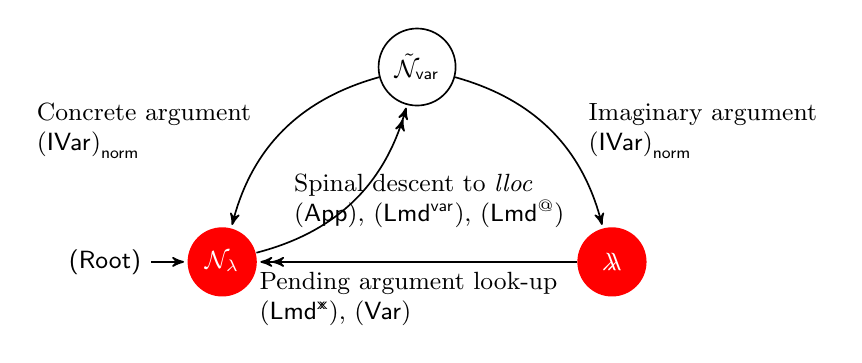
\begin{tikzpicture}[->,>=stealth',shorten >=1pt,auto,node distance=3.5cm,
    semithick,initial text=$${\sf  (Root)}$$,font=\small ]
\tikzstyle{every state}=[fill=red,draw=none,text=white]

\node[initial,state]
    (L) {$\NodesLmd $};
\node[state,fill=white,draw=black,text=black]
    (V) [above right of=L] {$\ExtendedNodesVar $};
\node[state] (G) [below right of=V] {$\ghostlmd $};

\path (L) edge [bend right,->>]      node[right,xshift=-2.5em,text width=4cm]{Spinal descent to \emph{lloc} ${\sf  (App)}$, ${\sf  (Lmd^{\sf  var})}$, ${\sf  (Lmd^{@})}$} (V)
      (V) edge [bend right]  node[left,text width=3cm] {Concrete argument $\mathbf {({\sf  IVar})}_{\normalizing} $} (L)
          edge [bend left]   node[right, xshift=1em, text width=3cm] {Imaginary argument $\mathbf {({\sf  IVar})}_{\normalizing} $} (G)
      (G) edge [->>]                 node[below,text width=4cm] {Pending argument look-up ${\sf  (Lmd^{\ghostvar}  )}$, $\mathbf {({\sf  Var})}$} (L)
;
\end{tikzpicture}
\end{sgmlfig}
\caption{Decomposition of normalizing traversals of a \emph{qnf}. Bottom
states (lambda/ghost lambda) and top state (variable) produce the external
nodes respectively delimiting the start and end of a strand. A double arrow
represents multiple uses of deterministic rules; a single arrow represents a
single rule instantiation of a non-deterministic
rule.}\label{fig:qnf_strand_decomposition_statemachine}
\end{figure}

We show by a finite induction on $i \in \{r, q\}$ proceeding bottom-up from
the lower tree node $\lambda \overline{z_{q}}$ up to $\lambda
\overline{z_{r}}$ that $k_{i}>|\lambda _{l}(\lambda \overline{z_{i}})|$. Base
case follows from $k>|x|$ since $\lambda \overline{y_{2}}$ is structural.
Suppose the result holds for $i\in \{r+1..q\}$. The lambda-list at $@_{i}$ is
obtained by popping $|@_{i}|$ lambdas from the lambda-list at $\lambda
\overline{z_{i}}$ and $\lambda _{l}(\lambda \overline{z_{i}})$ is by
definition $\overline{z_{i}}$ concatenated with the lambda-list of $@_{i+1}$,
hence $|\lambda _{l}(@_{i})| = \max ( 0, |\lambda _{l}(@_{i+1})| + |\lambda
\overline{z_{i}}| - |@_{i}| )$. We thus have $|\lambda _{l}(\lambda
\overline{z_{i-1}})| - k_{i-1} = |\lambda \overline{z_{i-1}}| +|\lambda
_{l}(@_{i})| - k_{i-1} = \max (  |@_{i}|- k_{i}, |\lambda _{l}(\lambda
\overline{z_{i}})| - k_{i} )$. By the induction hypothesis we have $|\lambda
_{l}(\lambda \overline{z_{i}})| < k_{i}$, and since nodes in $v$ are all
ghosts we have $|@_{i}|< k_{i}$ thus the `$\max $' is negative which shows
$|\lambda _{l}(\lambda \overline{z_{i-1}})| < k_{i-1}$. Since in particular
$|\lambda _{l}(\lambda \overline{z_{r}})| < k_{r}$, the application $(\lambda
\overline{z_{r}} . A_{0}) A_{1} \ldots A_{k_{r}-1}$ has more operands than
pending lambdas in the operator, thus its lambda list is empty. By
assumption, the strand is of type $S$ thus $lloc(\lambda
\overline{w_{1}})=\bot $ and since there is no \emph{lloc} ``left of''
$\lambda \overline{y_{2}}$, there cannot possibly be a \emph{lloc} under
$\lambda \overline{y_{2}}$. Hence $lloc(\lambda \overline{y_{2}}) =\bot $.
The same argument used in the \emph{structural argument} case shows that
 $u_{2}$ is a spinal descent. Hence the next strand is of type $G$.
\end{proof}

%p7.2 #&#
\begin{proposition}\label{prop:qnf_traversals_are_finite}
Let $t \in \travsetnorm (M)$ for some \emph{quasi normal} term $M$. We have:
%
\begin{enumerate}[\textit{(a)}]
\item[\textit{(a)}] $lloc_{M}(\nu ) = \bot $ for all external lambda node $\nu \in
    \NodesLmd $ occurring in $t$;
\item[\textit{(b)}] $t$ does not contain any internal variable node (\textit{i.e.},
    all the internal nodes are $@$ nodes);
\item[\textit{(c)}] $t$ is finite.
\end{enumerate}
\end{proposition}

\begin{proof}
(a) and (b) are direct consequences of
\reftext{Proposition~\ref{prop:qnf_strand_decomposition}}. For (c), let's
consider each case of the strand decomposition of
\reftext{Proposition~\ref{prop:qnf_strand_decomposition}}. For transitions
$\rightarrow S$ and $S \rightarrow S$, because $u_{1}$ and $u_{2}$ are spinal
descents, the last node in the next strand ($x_{1}$ or $x_{2}$) must be a
descendant in $\ctree (M)$ of the first node ($\lambda \overline{w_{1}}$)
from the previous strand. For transition $S\rightarrow G$, since both $u_{1}$
and $u_{2}$ are spinal descents, there are also paths in the tree, therefore
since $\lambda \overline{y_{2}}$ points to $u_{1}$, $x_{2}$ must also be a
descendant of $\lambda \overline{w_{1}}$. For transitions $G \rightarrow S$
and $G \rightarrow G$, since $u_{1}$ and $u_{2}$ are spinal descents, $x_{2}$
is a descendant of $\lambda \overline{y_{2}}$, itself a descendant of
$\lambda \overline{y_{1}}$. Suppose $t$ is infinite then from the strand
decomposition we can construct an infinite path in the tree of $M$ which
contradicts the fact that $M$ is a finitary term.
\end{proof}


%l7.3 #&#
\begin{lemma}[Generalized redex argument lookup]\label{lemma:genredex_lookup}
Let $x$ be a variable occurrence involved in a generalized redex in $gr(M)$.
%
\begin{enumerate}[\textit{(ii)}]
\item[\textit{(i)}] The path from the parent node of the redex argument down to
    $x$'s binder is of the form $ @_{r} \; \lambda \overline{x_{r}} \cdots
    @_{2} \; \lambda \overline{x_{2}} \; @_{1} \; \lambda \overline{x}$ for
    $r\geq 0$, where $@_{r}$ denotes the parent node of the redex argument,
    and $\lambda \overline{x}$ denotes $x$'s binder, such that $\lambda x$
    is the $i$th lambda in the bulk $\lambda \overline{x}$ for $i\geq 0$.

\item[\textit{(ii)}] The argument of $x$ is precisely given by the $i_{k}$th child
    of node $@_{k}$ where $k$ is the smallest index verifying
    $i_{k}<|@_{k}|$ where $i_{1} = i$ and $i_{j+1} = i_{j} - |@_{j}| +
    |\lambda \overline{x_{j+1}}|$ for $j\geq 0$.
\end{enumerate}
\end{lemma}

\begin{proof}
(i) By definition of $gr(M)$, $@_{r}$ necessarily occurs in the path from
$\lambda \overline{x}$ to the root, which is necessarily a spinal descent: if
it contained a variable $z$ the lambda-list at that node would be empty, and
no argument could possibly form a generalized redex with $\lambda x$. (ii) We
show by induction on $k$ that $x$ is the variable abstracted by the $i_{k}$th
lambda in $\lambda _{l}(\lambda \overline{x_{k}})$, which implies the result
since $\lambda x$ forms a generalized redex with the $i_{k}$th argument of
$@_{k}$. For $k=1$, by assumption, $\lambda x$ is the $i$th lambda in the
bulk lambda $\lambda \overline{x}$. For $k\geq 1$, by the I.H. $\lambda x$ is
the $i_{k-1}$ lambda in $\lambda _{l}(\lambda \overline{x_{k-1}})$. By
definition $k$ verifies $i_{k-1}\geq |@_{k-1}|$ therefore the
long-application $@_{k-1}$ has the effect of popping exactly $|@_{k-1}|$
arguments from the lambda-list, and the abstraction $\lambda
\overline{x_{k}}$ then adds $|\lambda \overline{x_{k}}|$ more lambdas in
front of it. Hence $\lambda x$ is positioned at $i_{k-1} - |@_{k-1}| +
|\lambda \overline{x_{k}}| = i_{k}$ in $\lambda _{l}(\lambda
\overline{x_{k}})$.
\end{proof}
%\proofatend
%(i) By definition of generalized redexes and lambda lists (Definition~\ref{dfn:generalized_redex}), $@_r$ necessarily occurs in the path from $\lambda \overline{x}$ to the root. Further the path from $@_r$ to $\lambda \overline{x}$ is necessarily a spinal descent (\textit{i.e.}, it contains only lambda and application nodes, and no variable node). Indeed, if it contained a variable node $z$ then the lambda-list at the subterm rooted at $z$ would be empty, in which case no argument could possibly form a generalized redex with $\lambda x$.
%
%(ii) We show by induction on $k$ that $x$ is the variable abstracted by the $i_k$th lambda in $\lambda _l(\lambda \overline{x_k})$, which implies the result since by definition $\lambda x$ forms a generalized redex with the $i_k$th argument of $@_k$.
%Base case $k=1$. By assumption, $\lambda x$ is the $i$th lambda in the bulk lambda $\lambda \overline{x}$. Let $k\geq 1$. By the induction hypothesis $\lambda x$ is the $i_{k-1}$ lambda in $\lambda _l(\lambda \overline{x_{k-1}})$.
%By definition of $k$ we have $i_{k-1}\geq |@_{k-1}|$, therefore by definition of $\lambda _l$, the long-application $@_{k-1}$ has the effect of popping exactly $|@_{k-1}|$ arguments from the lambda-list, and the following abstraction $\lambda \overline{x_k}$ then adds $|\lambda \overline{x_k}|$ more lambdas in front of the lambda list. Hence $\lambda x$ gets moved to position $i_{k-1} - |@_{k-1}| + |\lambda \overline{x_k}| = i_k$ in the lambda list at $\lambda \overline{x_k}$.
%\endproofatend

\paragraph*{Traversal bisimulation}
For $t, t' \in \travsetnorm (M)$ we write $t \rightarrow _{M} t'$ just if
$t'$ is an immediate extension of $t$ in $\travsetnorm (M)$, that is $t'$
extends $t$ via a single instantiation of the normalizing traversal rules;
and $t \internalextension _{M} t'$ if the node traversed by $t'$ is an
internal node. We write $\rightarrow _{M}^{*}$ and, $\internalextension
_{M}^{*}$ to denote their reflexive transitive closure. To simplify the
definition of bisimulation, we now assume that $\travsetnorm $ also contains
the empty justified sequence $\epsilon $, which was excluded in our
presentation of traversal rules, so that $\travsetnorm (M)$ is precisely the
transitive closure of $\{ \epsilon \}$ by $\rightarrow _{M}$.

\begin{definition}[Traversal bisimulation]\label{def:bisimilar_terms}
Two untyped terms $M$ and $N$ with variables in $\mathcal{V}$ are
\textbf{\emph{bisimilar}}\index{bisimilar} if for all $t_{1} \in \travsetnorm
(M)$, $u_{1} \in \travsetnorm (N)$ such that $\core{t_{1}} = \core{u_{1}}$ we
have:
%
\begin{itemize}[(B2)]
\item[(B1)] if $t_{1} \rightarrow _{M} t'$ then $t' \internalextension
    _{M}^{*} t_{2}$, $u_{1} \rightarrow ^{*}_{N} u_{2}$ with $\core{t_{2}}
    = \core{u_{2}}$ for some $t_{2}, u_{2}$;
\item[(B2)] if $u_{1} \rightarrow _{N} u'$ then $u' \internalextension
    _{N}^{*} u_{2}$, $t_{1} \rightarrow ^{*}_{M} t_{2}$ with $\core{t_{2}}
    = \core{u_{2}}$,
       for some $t_{2},u_{2}$.
\end{itemize}
\end{definition}

We write $\travsetscn (M)$ for the set of (finite) \textbf{\emph{normalizing
traversals with complete strands}}\index{normalizing traversals with complete
strands}.

\begin{lemma}\label{lem:bisimulation_isomorphism}
If $M$ and $N$ are bisimilar then $\coresymbol (\travsetscn (N)) =
\coresymbol (\travsetscn (M))$.
\end{lemma}

\begin{proof}
$\travsetnorm (N)$ is by definition the transitive closure by $\rightarrow
_{N}$ of the singleton traversal, so for any $u$ of $\travsetscn (N) \subset
\travsetnorm (N)$, repeatedly applying (B2) for each step of $u$'s
$\rightarrow _{N}$ derivation shows that there is $u' \in \travsetnorm (N)$
and  $t' \in \travsetnorm (M)$ such that $\core{u'} = \core{t'}$ and $u
\internalextension _{N}^{*} u'$. Take $t$ to be the longest prefix of $t'$
ending with an external variable, then by definition $t$ belongs to
$\travsetscn (M)$. And because the occurrences following $u$ in $u'$ are all
internal, $u$ is also the longest prefix of $u'$ ending with an external
node. Hence since $\core{u'} = \core{t'}$, by the definition of $\coresymbol
$ we necessarily have $\core{u} = \core{t}$, which shows that $\core{u}\in
\core{\travsetscn (M)}$. This gives the first inclusion. The proof of the
opposite inclusion is symmetrical.
\end{proof}

\begin{proposition}\label{prop:ulctrav_impl_linear_reduction}
If $M \llred N$ then $M$ and $N$ are bisimilar.
\end{proposition}

%
\begin{proof}[Proof overview]
Suppose that $M \llred N$. Let $x$ denote the \emph{lloc} in $M$ and
$(\lambda x, A)$ be the generalized redex involving it, so that $N$ is the
term obtained by firing $(\lambda x, A)$. A property of linear reduction is
that $M$ is a subterm of the reduct $N$. This induces a function $\Phi :
\ExtendedNodes (N) \rightarrow \ExtendedNodes (M)$ mapping nodes under the
substituted subterm in $N$ to the corresponding nodes under argument $A$ in
$M$, and every node in $N$ that is not involved in the substitution, to its
counterpart in $M$. The linear substitution can affect the term tree in three
ways depending on the arity of the \emph{lloc} and the structure of the
argument. We show bisimilarity for each case.


\begin{figure}
\begin{sgmlfig}
\begin{tikzpicture}[baseline=(root.base),level distance=16pt,inner ysep=0.5mm,sibling distance=7mm,font=\small ]
\node (root){}
        child[dashed]{node{$@_{a}$}
            child[solid]{node{$\lambda \overline{w_{a}}$}
                child[dashed]{node{$@_{a-1}$}
                    child{node{$\lambda \ldots $}
                        child[solid]{node{$@$}
                            child[solid]{node{$\lambda \overline{z}$}
                                child[solid,level distance=5ex]{node {$x$}
                                    child{node{$B_{1}$}}
                                    child{node{$\ldots $}}
                                    child{node{$B_{|x|}$}}
                                    }
                                edge from parent }
                            child[dashed]{node{}}
                        }
                    }
                    child[dashed]{node{}}
                }
                edge from parent }
            child[dashed]{node{\ldots }}
            child[solid]{node{$\lambda \overline{y}$}
                child{node{$R$}}
            }
            child[dashed]{node{\ldots }}
        }
;
\node (root2) at (5,0) {}
    child[dashed]{node{$@_{a}$}
        child[solid]{node{$\lambda \overline{w_{a}}$}
            child[dashed]{node{$@_{a-1}$}
                child{node{$\lambda \ldots $}
                    child[solid]{node{$@$}
                        child[solid]{node{$\lambda \overline{z}$}
                            child[solid,level distance=5ex]{node {$@_{x}$}
                                child{node{$\lambda \overline{y}'$}
                                    child{node{$R'$}}
                                }
                                child{node{$B_{1}$}}
                                child{node{$\ldots $}}
                                child{node{$B_{|x|}$}}
                                }
                            edge from parent }
                        child[dashed]{node{}}
                    }
                }
                child[dashed]{node{}}
            }
            edge from parent }
        child[dashed]{node{\ldots }}
        child[solid]{node{$\lambda \overline{y}$}
            child{node{$R$}}
        }
        child[dashed]{node{\ldots }}
    }
;
\draw [<-] ([xshift=1.6cm,yshift=-2cm]root.east) -- +(1cm,0)
node[midway, above] {$\Phi $};
\draw [->] ([xshift=1.6cm,yshift=-1cm]root.east) -- +(1cm,0)
node[midway, above] {$\llred $};
\end{tikzpicture}
\end{sgmlfig}
\caption{$M\llred N$ Linearly firing the generalized redex in $M$ (left) yields
$N$ (right) where $R'$ denotes a copy of $R$.}\label{fig3}
\end{figure}

\textbf{Case 1:} $x$ has at least one operand ($|x|>0$) and $A$ is an
abstraction. Let $@_{j}$ and $\lambda \overline{w_{j}}$ for $1\leq j\leq a$,
$a\geq 1$ denote respectively the @-nodes and $\lambda $-nodes in the spinal
descent from $@_{a}$ to $x$'s binder where $@_{a}$ denotes the parent node of
the argument $A = \lambda \overline{y}. R$. So that $\lambda
\overline{w_{1}}$ is $x$'s binder and $@_{1}$ its parent. Let $i$ denote
$x$'s binding index in $\lambda \overline{w_{1}}$. After reduction, node $x$
gets replaced by an application node $@_{x}$; its existing children are
preserved; and a new subterm $\lambda \overline{y}'. R'$, a copy of the
subterm tree $A$, gets attached as the $0$th child tree of $@_{x}$. The copy
preserves the original variable names from $R$, which does not cause capture
since the variable binding is uniquely determined by the enabling relation.
We write $\lambda \overline{y}'$, priming the node label, to distinguish the
root of $R'$ from that of $R$, although they are both labelled with variable
names $\overline{y}$. We thus have $\Phi (@_{x}) = x$, $\Phi (\lambda
\overline{y}') = \lambda \overline{y}$, and $\Phi $ maps each node from
subterm $\lambda \overline{y}'. R'$  to the corresponding node under $\lambda
\overline{y}.R$.


(i) $\Phi $ preserves the enabling relation: if $n_{1} \enables _{i} n_{2}$
in $N$ for $i\geq 0$, $n_{1},n_{2} \in \Nodes (N)$ then $\Phi (n_{1})
\enables _{i} \Phi (n_{1})$ as long as $(n_{1},n_{2}) \neq (@_{x},\lambda
\overline{y}')$. Indeed, $\Phi $ preserves the parent-child relation for all
nodes except $@_{x}$: the child nodes of their image by $\Phi $ are the image
of their children; and $\Phi $ preserves variable binding: it maps the binder
of a variable node $z$ in $N$ to the binder of $\Phi (z)$ in $M$ with same
variable index;

(ii) $\Phi $ preserves node types: external nodes map to external nodes,
internal nodes map to internal nodes; $\lambda $-nodes map to $\lambda
$-nodes; a variable or @-node maps to either a variable or an @-node; ghosts
map to ghosts; and structural nodes map to structural nodes;

(iii) $\Phi $ preserves arity, in particular $|x| = |@_{x}|$ since $@_{x}$'s
operator does not contribute to its arity; (iv) $\Phi $ is not injective:
since nodes under $R$ and $R'$ map pairwise to the same node under $R$ in
$M$\xch{ (\reftext{Fig.~\ref{fig3}}).}{.}

We define the function $\phi $ on $\travsetnorm (N)$ that maps occurrences
pointwise by $\Phi $, preserves all justification pointers except for $@_{x}$
and $\lambda \overline{y}'$, and inserts after each occurrence of the
\emph{lloc} $x$, the corresponding \emph{argument lookup} of $x$. It adjusts
justification pointers as follows: for $n\notin \{ @_{x}, \lambda
\overline{y} \}$, $\Phi (n)$ has the same link distance and label as $n$; if
$n$ is an occurrence of $x$ then $\Phi (n)$ points to the first occurrence of
$x$'s binder in $\ulcorner  \phi  (u) \urcorner  $ and has link label $i$; if
$n$ is an occurrence of $\lambda \overline{y}'$ then  $\Phi (n)$ points to
the last occurrence of $@_{a}$ in $\ulcorner  \phi  (u) \urcorner  $ with
link label $i$. This is well-defined since by the P-view-path correspondence,
$x$'s binder (resp.\ $@_{a}$) necessarily occurs in the P-view at $x$ (resp.\
$\lambda \overline{y}'$). Between every occurrence of the \emph{lloc} $x$ and
$\lambda \overline{y}$, it inserts the \emph{argument lookup} sequence
consisting of ghost nodes statically determined by the term tree and obtained
by repeatedly instantiating rules $\mathsf{(Lmd)}$ and $\mathsf{(Var)}$. So
that a traversal of the shape $u = \raisebox{-2pt}{\includegraphics{12154i39}}$ of $N$ maps to
$\phi (u) = \raisebox{-2pt}{\includegraphics{12154i40}}$. The transformation does not affect
the structure of the core projection because it only inserts internal nodes,
and alters the justification pointers of internal occurrences $@_{x}$ and
$\lambda \overline y$ only, whereas justified sequences in $\coresymbol
(\travsetnorm (N))$ do not contain any internal node. We define $\varphi
^{-1}$ as the reverse transformation that removes all the occurrences between
the \emph{lloc} $x$ and the  argument $\lambda $-node $\lambda \overline{y}$.
We show simultaneously that $\rightarrow _{M}$ simulates $\rightarrow _{N}$
and that the simulating traversal in $M$ is the image by $\varphi $ of the
simulated traversal of $N$, and reciprocally that $\rightarrow _{N}$
simulates $\rightarrow _{M}$ via $\varphi ^{-1}$. The proof goes by induction
on and case analysis on the rule used to extend the traversal.




\textbf{Case 2:} $x$ has at least one operand ($|x|>0$) and $A = \lambda . R$
where $A$'s root node is the dummy lambda. The root node $r$ of $R$ is either
a variable if it is in head-normal form, or an $@$-node. The tree $\ctree
(N)$ is obtained from $\ctree (M)$ by substituting $x$'s label with that of
$r$ and prepending $r$'s children to existing $x$'s children. Other nodes,
including $x$'s parent $\lambda $-node, remain untouched. Let $r'$ denote
this node in the reduct $N$. This transformation yields an implicit mapping
function $\Phi : \ExtendedNodes (N)\rightarrow \ExtendedNodes (N)$ such that
$\Phi (r') = x$. Although $\Phi $ does not preserve the arity of $x$, it does
not affect the dynamic arity of traversals since $|r'| = |x| + |r|$. We then
show by induction and case analysis on the rules that the two terms are
bisimilar.

\textbf{Case 3:} $x$ is unapplied ($|x|=0$). After reduction, node $x$ gets
replaced by subterm $A$ and the label of $x$'s parent $\lambda $-node gets
concatenated with the label of $A$'s root node: the parent node $\lambda
\overline{z}$ of $x$ in $M$ becomes $\lambda \overline{z}\overline{y}'$ in
the reduct $N$. A traversal of $M$ of the form $\ldots \lambda \overline{z}
\cdot x \cdot v \cdot \lambda \overline{y} \ldots $, where $v$ is an argument
lookup, can be bisimulated by traversals in $N$ of the form $\ldots \lambda
\overline{z}\overline{y}' \ldots $ The arity of $x$ is not preserved but it
does not alter the dynamic arity because $|\lambda{\overline{z}
\overline{y}'}| = |\lambda{\overline{z}}| +  |\lambda{\overline{y}}|$.
\end{proof}


\begin{proposition}\label{prop:ulctrav_sound_for_trivialreduction}
Let $M$ be an untyped term containing only trivial redexes, and $N$ the
reduct obtained by firing the \emph{leftmost spinal-innermost} trivial redex,
then $M$ and $N$ are bisimilar.
\end{proposition}

\begin{proof}[Proof overview]
The figure below shows the tree structure at a subterm $(\lambda \overline{x}
. T) A_{1} \ldots A_{r}$ for $r\geq 1$ where $(x_{1}, A_{1})$ forms the
leftmost spinal-innermost trivial redex. Two cases must be considered:

\begin{center}
            \begin{tikzpicture}[baseline=(root.base),level distance=4ex,inner ysep=0.5mm,sibling distance=8mm]
                \node (root_rGt1_M){}
                        child[dashed]{node{$\lambda \overline{w}$}
                            child[solid]{node{$@$}
                                child[solid]{
                                    node{$\lambda \overline{x}$}
                                    child[solid,level distance=5ex]
                                        {node {$T$}}
                                    edge from parent }
                                child{node{$A_{1}$}}
                                child[dashed]{node{$\ldots $}}
                                child{node{$A_{r}$}}
                            }
                        };
                \node (root_rGt1_N) at (4.5,0) {}
                        child[dashed]{node{$\lambda \overline{w}$}
                            child[solid]{node{$@$}
                                child[solid]{
                                    node{$\lambda x_{2} \ldots x_{n}\qquad $}
                                    child[solid,level distance=5ex]
                                        {node {$T$}}
                                    edge from parent }
                                child{node{$A_{2}$}}
                                child[dashed]{node{$\ldots $}}
                                child{node{$A_{r}$}}
                            }
                        };
                \node (root_rEq1_M) at (8,0) {}
                        child[dashed]{node{$\lambda \overline{w}$}
                            child[solid]{node{$@$}
                                child[solid]{
                                    node{$\lambda \overline{x}$}
                                    child[solid,level distance=5ex]
                                        {node {$T$}}
                                    edge from parent }
                                child{node{$A_{1}$}}
                            }
                        };
                \node (root_rEq1_N) at (12,0) {}
                        child[dashed]{node{$\lambda \overline{w}~x_{2} \ldots x_{n}$}
                            child[solid]{node{$T$}
                            }
                        }
                ;
                \draw [->] ([xshift=1.5cm,yshift=-1cm]root_rGt1_M.east) --
                +(1.5cm,0)
                node[midway, above, text width=1.5cm,font=\small ] {\mbox{trivial} \mbox{reduction}};
                \draw [->] ([xshift=1cm,yshift=-1.5cm]root_rEq1_M.east) --
                 +(1.5cm,0)
                    node[midway, above, text width=1.5cm,font=\small ] {\mbox{trivial} \mbox{reduction}} ;
                \end{tikzpicture}
            \end{center}
\noindent \emph{Case $r>1$ (left)} The reduct tree is a subtree of the
original tree modulo minor relabelling. This induces an injection $\Phi $
from nodes of $N$ to nodes of $M$. Extending it occurrence-wise to justified
sequences yields a bisimulation between $M$ and $N$. This is because: (i)
Since $x_{1}$ does not occur in $T$, $A_{1}$ will never be traversed in $N$.
(ii) Only occurrences hereditarily justified by $\lambda x_{1} \ldots x_{n}$
have their link label changed, when simulating a traversal of $N$ in $M$. But
since they are internal they are filtered out by $\coresymbol $. (iii) The
arity of $\lambda x_{2} \ldots x_{n}$ increases by $1$ after applying $\Phi
$, but the arity of the @-node also increases by $1$ so it does not alter the
dynamic arity of traversals. (iv) The bisimulation preserves the core: by an
easy induction, observing that $@$ and $\lambda x_{2}\ldots x_{n}$ must occur
consecutively in a traversal of $N$ and the sum of their arity is preserved
by $\Phi $.

\emph{Case $r>1$ (right)} The tree of $N$ is obtained by removing the @-node
and argument $A_{1}$ and combining the two $\lambda $-nodes into $\lambda
\overline{y}$ where $\overline{y} = \overline{w} x_{2} \ldots x_{n}$. This
induces an injection $\Phi $ from nodes of $N$ to nodes of $M$. We
simultaneously and inductively define a bijection $\varphi $ from $\mathcal
{T}\!rav_{\normalizing} (N)$ to a subset of $\mathcal {T}\!rav_{\normalizing}
(M)$ and that $\rightarrow _{M}$ simulates $\rightarrow _{N}$ via $\varphi $
and reciprocally. The base case is immediate; we treat the interesting case
of the induction: $u_{1}$ and $t_{1}=\varphi (u_{1})$ are respectively
traversals of $N$ and $M$ such that $\core{u_{1}} = \core{t_{1}}$. If $u_{1}
\rightarrow _{N} u_{1} \cdot \lambda \overline{y} = u'$ then we extend $u'
\internalextension _{N} u_{1} \cdot \lambda \overline{y} \cdot s \cdot z = u$
where $s$ is the spinal descent in $T$ and $z$ is the \emph{hoc} of $T$. The
sequence $t' = t_{1} \cdot \lambda \overline{w} ~ @ ~ \lambda \overline{x}
\cdot \Phi (s) \cdot \Phi (z)$ where $\Phi (s)$ denotes the pointwise
extension of $\Phi $, is clearly a traversal extension of $t_{1}$ in $M$.
Because $|\lambda \overline{w}| - |@| + |\lambda \overline{x}| =|\lambda
\overline{y}| $, the core calculation on $t'_{\leq \lambda \overline{x}}$
adequately and discharge pending lambdas names $x_{2} \ldots x_{n}$ onto node
$\lambda \overline{w}$. To prove that the simulation preserves $\core{\_}$ it
suffices to show that occurrences following $\lambda \overline{x}$ in $t'$
and those following $\lambda \overline{y}$ in $u$ yield the same pending
lambdas, and that the last occurrence in the two traversals are either both
internal or both external. If $z$ is internal then since $s$ and $\varphi
(s)$ are both  spinal descent of $T$, they have the same bound variables and
arities thus we have $\core{u} = \core{t'}$. If $z$ is external and its
justifier is not $\lambda \overline{w}$ then $\Phi (z)$ is also external and
again $\core{u} = \core{t'}$. If $z$ is external and justified by $\lambda
\overline{w}$ with link label $j<|\overline{w}|$ then $\Phi (z)$ is
necessarily external and $\core{u} = \core{t'}$. For those three cases we
define $\varphi (u) = t'$. If $z$ is external and is justified by $\lambda
\overline{w}$ with link label $|\overline{w}|<j\leq |\overline{w}| + n -1$
then $z$ and $\Phi (z)$ are both labelled by the variable $x_{i}$ where
$i=j-|\overline{w}|+1$, and therefore node $\Phi (z)$ is bound by $\lambda
\overline{x}$ in $M$ and is thus external. To simulate $u'$ we extend $t'
\rightarrow ^{*}_{M} t = t' \cdot (\ghostlmd \, \ghostvar )^{k}$ where
$(\ghostlmd \, \ghostvar )^{k}$ is the argument lookup of $z$ for $k>0$ and
the last $\ghostvar $ points to $\lambda \overline{w}$ with label $j$. We
then have $t_{1} \rightarrow ^{*}_{M} t$, $u'\internalextension _{N} u$ and,
since ghosts all have null arity, $\core{u} = \core{t}$. We define $\varphi
(u) = t$. This is the situation where a ghost variable in $M$ gets
materialized into a variable occurrence ($x_{i}$) in $N$. Reciprocally, if
$t_{1} \rightarrow _{M} t_{1} \cdot \lambda \overline{w}$ then $t_{1} \cdot
\lambda \overline{w} \internalextension _{M} t' = \raisebox{-2pt}{\includegraphics{12154i41}}
$ where $i\geq 1$, $k\geq 0$, $s$ is the spinal descent in $M$ and
$(\ghostlmd \, \ghostvar )^{k+1}$ is the argument lookup, and $t'$ is
simulated by $\phi ^{-1}(t') = \raisebox{-2pt}{\includegraphics{12154i42}} $ where $v =
\ghostvar $ if $i>n$, and $v = x_{i}$ otherwise.
\end{proof}


\begin{example}
Take the term $M = \lambda x. (\lambda y z.z) u$ which trivially reduces to
$N = \lambda x z . z$. The normalizing traversal ${\includegraphics{12154i43}}$
of $N$ simulates traversal $t$ of $M$ from
\reftext{Example~\ref{examp:ghost_materialization}}.
\end{example}


\begin{corollary}\label{cor:qnf_and_nf_traveset_invariant}
If $M$ is in \emph{qnf} and has $\beta $-normal form $N$ then $\coresymbol
(\travsetscn (M)) \cong \coresymbol (\travsetscn (N))$.
\end{corollary}

\begin{proof}
By \reftext{Proposition~\ref{prop:qnf_nf}}(ii) there is a reduction sequence
$M = M_{1} \rightarrow _\beta \ldots \rightarrow _\beta M_{q}$, $q\geq 1$
where in each step, $M_{i+1}$ is obtained by reducing the leftmost
spinal-innermost standard redex of $M_{i}$, and $M_{q}$ is $\alpha
$-equivalent to $N$. By \reftext{Proposition~\ref{prop:qnf_nf}}(i), each such
redex is trivial, so by
\reftext{Proposition~\ref{prop:ulctrav_sound_for_trivialreduction}} the
reducts in the sequence are all bisimilar, and by
\reftext{Lemma~\ref{lem:bisimulation_isomorphism}}, $\core{\travsetscn (M)} =
\core{\travsetscn (M_{q})}$. Since $M_{q}$ is $\alpha $-equivalent to $N$ we
have the desired structure-preserving isomorphism.
\end{proof}

\begin{proposition}\label{prop:ulc_travnorm_finite}
Let $M$ be an untyped term with a beta-normal form. Then (i) All traversals
in $\travsetnorm (M)$ are finite; (ii) The set $\travsetnorm (M)$ is finite.
\end{proposition}

\begin{proof}
(i) If $M$ has a normal form then by
\reftext{Theorem~\ref{thm:completeness_leftmostlinearred}} its linear
reduction sequence yields a quasi-normal form $Q$ which by
\reftext{Theorem~\ref{thm:soundness_leftmostlinearred}} is beta-equivalent to
$M$. Thus, by \reftext{Proposition~\ref{prop:ulctrav_impl_linear_reduction}}
the maximal traversals of $M$ and $Q$ are isomorphic. So if $M$ has an
infinite traversal then so does $Q$, which contradicts
\reftext{Proposition~\ref{prop:qnf_traversals_are_finite}}. (ii) Traversals
rules defining $\travsetnorm $ all have bounded non-determinism therefore by
(i) $\travsetnorm $ is finite.
\end{proof}

\begin{theorem}[ULC normalized paths characterization]\label{thm:path_charact_ulc}
Let $M$ be an untyped term with normal form $T$. We have $\travsetscn
(M)/{\sim } \, \structisomorphic \, \pathset (T)$.
\end{theorem}

\begin{proof}
Suppose first that $M$ is in $\beta $-nf. Then its tree has no $@$-node and
all nodes are external. Hence the dynamic arity of a traversal ending with
external variable $x$ is precisely the arity of $x$. Since all nodes are
external, rule $\mathsf{(Var)}$ is never used and we have $\travsetnorm (M) =
\travsetscn (M) = \pathset (M)$. Further the projection $\coresymbol $
coincides with the identity thus $\core{\travsetnorm (M)} = \travsetnorm (M)
= \pathset (M)$. If $M$ is not a normal form then since $M$ has a $\beta
$-nf, by \reftext{Theorem~\ref{thm:completeness_leftmostlinearred}} its
\emph{leftmost linear reduction sequence} terminates and yields a \emph{qnf}.
By \reftext{Proposition~\ref{prop:ulctrav_impl_linear_reduction}}, the
reducts are all bisimilar with $M$, thus so is its \emph{qnf}. We then
conclude with \reftext{Lemma~\ref{lem:bisimulation_isomorphism}} and
\reftext{Corollary~\ref{cor:qnf_and_nf_traveset_invariant}}.
\end{proof}

\begin{proposition}\label{prop:core_travsetnorm_alpha_consistent}
$\core{\travsetscn (M)}$ is $\alpha $-consistent.
\end{proposition}

\begin{proof}
By definition, a traversal of $\travsetscn $ is finite and must end with an
external variable node. It is uniquely defined by the sequence of
non-deterministic choices of the argument index $i$ made at the end of each
strand. By \reftext{Theorem~\ref{thm:path_charact_ulc}}, this sequence of
indices also determines the path to the corresponding node in the tree of the
normal form. Hence for any two maximal traversals $t_{1},t_{2} \in
\travsetnorm $ ending with strands $\lambda \overline{x}_{1} \ldots y_{1}$
and $\lambda \overline{x}_{1} \ldots y_{1}$, if the sequence of argument
indices leading to $\lambda \overline{x}_{1}$ and $\lambda \overline{x}_{2}$
differ then they must refer to distinct tree nodes of the normal form. If
they are identical--all the non-deterministic choices leading to $\lambda
\overline{x}_{1}$ and $\lambda \overline{x}_{2}$ are the same--then we must
have $t_{\leq \lambda \overline{x}_{1}} = t_{\leq \lambda \overline{x}_{2}}$,
which by the deterministic traversal rules extends to $t_{1} = t_{2}$. Hence
$\core{t_{1}} = \core{t_{2}}$ and thus $\lambda \overline{x}$ and $\lambda
\overline{y}$ are assigned the same list of variable names in $\core{t_{1}}$
and $\core{t_{2}}$.
\end{proof}

\begin{proposition}
\reftext{Algorithm~\ref{algo:ulc_normalization_by_traversals}} is correct.
\end{proposition}

\begin{proof}
\emph{Termination}  By \reftext{Proposition~\ref{prop:ulc_travnorm_finite}}
there is a finite number of normalizing traversals and each of them can be
obtained with finitely many applications of traversal rules. \emph{Soundness}
follows from \reftext{Theorem~\ref{thm:path_charact_ulc}} and because a term
is characterized by its justified paths
(\reftext{Property~\ref{prop:tree_path_charact}}).
\reftext{Proposition~\ref{prop:core_travsetnorm_alpha_consistent}} implies
that the set of cores of (necessarily finite) maximal traversals of $M$ is
$\alpha $-consistent, so we can apply the readout procedure of
\reftext{Proposition~\ref{proposition:termtree_readout_from_justitied_paths}}
to reconstruct the $\beta $-normal form.
\end{proof}



\section{Further directions}\label{sec8}


\paragraph*{Reduction strategies}
We have seen that traversals implement leftmost linear reduction, a
non-strict non-standard reduction strategy that substitutes variables one at
a time. This begs the question of whether alternative notions of traversals
exist for other evaluation strategies, such as call-by-name and
call-by-value~\cite{plotkin-75}. A call-by-name variant, which does not fire
redexes inside the body of an unapplied abstraction, would easily be
accommodated for. A strict evaluation strategy like call-by-value, on the
other hand, might require substantial changes. For traditional reduction
strategies, such as the normal order of lambda calculus, this might require
non-deterministically spawning new traversals for every occurrence of the
variable involved in a redex.

\paragraph*{Game semantics}
We conjecture a result similar to
\reftext{Theorem~\ref{thm:gamesem_correspondence_stlc}} for the untyped case:
there is an isomorphism between the cores of imaginary traversals and the
innocent \emph{effectively almost everywhere copycat (EAC)} game denotation
of untyped lambda terms~\cite{KerThesis}, as well as an isomorphism between
the imaginary traversals and the EAC denotations that preserves internal
moves during composition. We suspect that a connection exists between the
`on-the-fly eta-expansion' of traversals and the morphism $Fun : U
\rightarrow (U \Rightarrow U)$ of Ker's game category, where $U$ is the
maximal game arena of the EAC strategies.


\paragraph*{Optimality and compilation}
\reftext{Example~\ref{tab:varity2_trav}} shows that traversals may get long
even for relatively simple terms. It is not surprising given that they were
not designed with efficiency in mind, but rather inspired by Game Semantics.
Traversals are clearly not L\'{e}vy-optimal~\cite{optimal-reduction-levy}: they
do exhibit some sharing through their use of pointers, which avoids copying
or rewriting subterms when evaluating redexes, but they make no attempt to
exploit such sharing to avoid redundant work. Traversing $(\lambda x. y x x)
A$, for instance, involves traversing $A$ for both occurrences of $x$, and if
that involves traversing a redex in $A$ the first time then that redex gets
traversed again the second time. On the other hand, traversals are
``hyper-lazy''~\cite{danosherbelinregnier1996}: they evaluate (generalized)
redexes one variable occurrence at a time and only when needed. So besides
the above-mentioned  redundancy, no useless work is performed, contrary to
the traditional evaluation of redexes that substitutes \emph{all} variable
occurrences even those that are dead-code. We might not be too far from
optimality: memoization techniques could conceivably shorten traversals and
possibly gain optimality by detecting shared L\'{e}vy-families of redexes as
they unfold. This perhaps relates to a remark by Danos and Regnier that
memoization can make \emph{Jumping Abstract Machines}
optimal~\cite{DANOS199979}. Despite the lack of optimality, traversals have
potential applications to program compilation, such as partial evaluation, an
avenue pursued by Berezun and Jones for their own notion of
traversals~\cite{berezunjones_partialevalbytraversals}.





%%% PASTABA: Pagal zurnalo ypatumus, reikalinga
%%%          zemiau esanti aplinka {conflict}.
%%%          Koduojama FLA, REV, SCO, DIS tipams.
%%%          S5 etapui koduoti NEREIKIA.

\begin{conflict}
None declared.
\end{conflict}





\begin{acks}
This work got inspired by slides of a talk by Daniil Berezun and Neil
D.~Jones~\cite{berezunjones_partialevalbytraversals}. It benefited from
communications with the authors and memorable discussions with Neil D.~Jones
during a visit at Microsoft in May 2017. An anonymous referee provided
valuable comments.
\end{acks}

%\begin{appm}
%\def\the...{}
%\reset{}{}
%\appendix{}
%\appendix*{}
%\end{appm}%
%spell_to        ********** End of text entry *****************
%
\begin{backmatter}%
% structpyb loaded by karolis.kavaliauskas, 2019-09-16 13:13:53
\begin{thebibliography}{}

%b1 ###
\bibitem{Abr02}
\begin{bsubitem}
\begin{bcontribution}%[language=fr]%de,it,pl,ru
\bauthor{\fnm{S.} \snm{Abramsky}}
\btitle{Algorithmic game semantics: a tutorial introduction}
\end{bcontribution}
\begin{bhost}
\begin{beditedbook}
\btitle{Proceedings of Marktoberdorf International Summer School}
\bdate{2001}
\end{beditedbook}
\end{bhost}
\end{bsubitem}
%
\OrigBibText
S.~Abramsky.
 Algorithmic game semantics: a tutorial introduction.
 In \emph{Proceedings of Marktoberdorf International Summer School},
 2001.
\endOrigBibText
\bptok{structpyb}%
\endbibitem

%b2 ###
\bibitem{Barendregt84}
\begin{bsubitem}
\begin{bcontribution}%[language=fr]%de,it,pl,ru
\bauthor{\fnm{H.P.} \snm{Barendregt}}
\btitle{The Lambda Calculus -- Its Syntax and Semantics}
\end{bcontribution}
\begin{bhost}
\begin{bbook}
\bbookseries{
\bseries{\btitle{Studies in Logic and the Foundations of Mathematics}\bvolumeno{103}}}
\bdate{1984}
\bpublisher{\bname{North-Holland}}
\end{bbook}
\end{bhost}
\end{bsubitem}
%
\OrigBibText
H.~P. Barendregt.
 \emph{{The Lambda Calculus -- Its Syntax and Semantics}}, volume 103
 of \emph{Studies in Logic and the Foundations of Mathematics}.
 North-Holland, 1984.
\endOrigBibText
\bptok{structpyb}%
\endbibitem

%b3 ###
\bibitem{berezunjones_partialevalbytraversals}
\begin{botherref}
D. Berezun,
N.D. Jones,
Partial evaluation and normalization by traversals,
January 2016,
Ga{L}o{P} workshop talk
\end{botherref}
%
\OrigBibText
D.~Berezun and N.~D. Jones.
 Partial evaluation and normalization by traversals (January 2016).
 Ga{L}o{P} workshop talk.
\endOrigBibText
\bptok{structpyb}%
\endbibitem

%b4 ###
\bibitem{JonesBerezunLLL-PEPM17}
\begin{bsubitem}
\begin{bcontribution}%[language=fr]%de,it,pl,ru
\bauthor{\fnm{D.} \snm{Berezun}}
\bauthor{\fnm{N.D.} \snm{Jones}}
\btitle{Compiling untyped lambda calculus to lower-level code by game
semantics and partial evaluation (invited paper)}
\end{bcontribution}
\begin{bhost}
\begin{beditedbook}
\btitle{Proc. PEPM}
\bdate{2017}
\bpublisher{\bname{ACM}}
\end{beditedbook}
\bpages{\bfirstpage{1}\blastpage{11}}
\end{bhost}
\end{bsubitem}
%
\OrigBibText
D.~Berezun and N.~D. Jones.
 Compiling untyped lambda calculus to lower-level code by game
 semantics and partial evaluation (invited paper).
 In \emph{Proc.\ PEPM}, pages 1--11. ACM, 2017.
\endOrigBibText
\bptok{structpyb}%
\endbibitem

%b5 ###
\bibitem{Blum-HogTool}
\begin{bsubitem}
\begin{bcontribution}%[language=fr]%de,it,pl,ru
\bauthor{\fnm{W.} \snm{Blum}}
\btitle{A Tool for Constructing Structures Generated by Higher-Order
Recursion Schemes and Collapsible Pushdown Automata}
\end{bcontribution}
\bcomment{Technical report}\prnsep{,\ }
\begin{bhost}
\begin{bbook}[class=report]
\bdate{2007}
\end{bbook}
\end{bhost}
\begin{bhost}
\begin{behost}
\binterref[locator-type=url,locator=http://github.com/blumu/dphil.tools]{github.com/blumu/dphil.tools}
\end{behost}
\end{bhost}
\end{bsubitem}
%
\OrigBibText
W.~Blum.
 A tool for constructing structures generated by higher-order
 recursion schemes and collapsible pushdown automata.
 \emph{Technical report}, 2007 www.github.com/blumu/dphil.tools.
\endOrigBibText
\bptok{structpyb}%
\endbibitem

%b6 ###
\bibitem{BlumGalop2008}
\begin{botherref}
W. Blum,
A concrete presentation of game semantics,
2008,
Ga{L}o{P} workshop talk
\end{botherref}
%
\OrigBibText
W.~Blum.
 A concrete presentation of game semantics.
 Ga{L}o{P} workshop talk, 2008.
\endOrigBibText
\bptok{structpyb}%
\endbibitem

%b7 ###
\bibitem{Blum-LocalBeta2008}
\begin{bsubitem}
\begin{bcontribution}%[language=fr]%de,it,pl,ru
\bauthor{\fnm{W.} \snm{Blum}}
\btitle{Local Computation of Beta-Reduction}
\end{bcontribution}
\bcomment{Technical report}\prnsep{,\ }
\begin{bhost}
\begin{bbook}[class=report]
\bdate{2008}
\bpublisher{\bname{University of Oxford}}
\end{bbook}
\end{bhost}
\end{bsubitem}
%
\OrigBibText
W.~Blum.
 Local computation of beta-reduction.
 Technical report, University of Oxford, 2008.
\endOrigBibText
\bptok{structpyb}%
\endbibitem

%b8 ###
\bibitem{BlumPhd}
\begin{bsubitem}
\begin{bcontribution}%[language=fr]%de,it,pl,ru
\bauthor{\fnm{W.} \snm{Blum}}
\btitle{The Safe Lambda Calculus}
\end{bcontribution}
\bcomment{PhD thesis}\prnsep{,\ }
\begin{bhost}
\begin{bbook}[class=report]
\bdate{2009}
\bpublisher{\bname{University of Oxford}\blocation{UK}}
\end{bbook}
\end{bhost}
\begin{bhost}
\begin{behost}
\binterref[locator-type=url]{https://ora.ox.ac.uk/objects/uuid:537d45e0-01ac-4645-8aba-ce284ca02673}
\end{behost}
\end{bhost}
\end{bsubitem}
%
\OrigBibText
W.~Blum.
 \emph{The Safe Lambda Calculus}.
 PhD thesis, University of Oxford, UK, 2009.
 https://ora.ox.ac.uk/objects/uuid:537d45e0-01ac-4645-8aba-ce284ca02673.
\endOrigBibText
\bptok{structpyb}%
\endbibitem

%b9 ###
\bibitem{BlumTypeScriptTraversal2019}
\begin{bsubitem}
\begin{bcontribution}%[language=fr]%de,it,pl,ru
\bauthor{\fnm{W.} \snm{Blum}}
\btitle{Traversing lambda-terms in TypeScript}
\end{bcontribution}
\begin{bhost}
\begin{behost}
\binterref[locator-type=url,locator=http://github.com/blumu/travnorm]{github.com/blumu/travnorm}
\bdate{2019}
\end{behost}
\end{bhost}
\end{bsubitem}
%
\OrigBibText
W.~Blum.
 Traversing lambda-terms in {T}ype{S}cript (2019).
 www.github.com/blumu/travnorm.
\endOrigBibText
\bptok{structpyb}%
\endbibitem

%b10 ###
\bibitem{curry_combinatorylogic}
\begin{bsubitem}
\begin{bcontribution}[language=de]%de,it,pl,ru
\bauthor{\fnm{H.B.} \snm{Curry}}
\btitle{Grundlagen der kombinatorischen logik}
\end{bcontribution}
\begin{bhost}
\begin{bissue}
\bseries{\btitle{Am. J. Math.} \bvolumeno{52}}
\bissueno{3}
\bdate{1930}
\end{bissue}
\bpages{\bfirstpage{509}\blastpage{536}}
\end{bhost}
\end{bsubitem}
%
\OrigBibText
H.~B. Curry.
 Grundlagen der kombinatorischen logik.
 \emph{American Journal of Mathematics}, 52(3):509--536, 1930.
\endOrigBibText
\bptok{structpyb}%
\endbibitem

%b11 ###
\bibitem{danosherbelinregnier1996}
\begin{bsubitem}
\begin{bcontribution}%[language=fr]%de,it,pl,ru
\bauthor{\fnm{V.} \snm{Danos}}
\bauthor{\fnm{H.} \snm{Herbelin}}
\bauthor{\fnm{L.} \snm{Regnier}}
\btitle{Game semantics and abstract machines}
\end{bcontribution}
\begin{bhost}
\begin{beditedbook}
\btitle{Proceedings of the Eleventh Annual IEEE Symposium on Logic in Computer Science, 1996}
\bconference{LICS '96}
\bdate{27--30 July 1996}
\end{beditedbook}
\bpages{\bfirstpage{394}\blastpage{405}}
\end{bhost}
\end{bsubitem}
%
\OrigBibText
V.~Danos, H.~Herbelin, and L.~Regnier.
 Game semantics and abstract machines.
 In \emph{Proceedings of the Eleventh Annual IEEE Symposium
 on Logic in Computer Science, 1996. LICS '96}, pages 394--405 (27-30 July 1996).
\endOrigBibText
\bptok{structpyb}%
\endbibitem

%b12 ###
\bibitem{DANOS199979}
\begin{bsubitem}
\begin{bcontribution}%[language=fr]%de,it,pl,ru
\bauthor{\fnm{V.} \snm{Danos}}
\bauthor{\fnm{L.} \snm{Regnier}}
\btitle{Reversible, irreversible and optimal $\lambda $-machines}
\end{bcontribution}
\begin{bhost}
\begin{bissue}
\bseries{\btitle{Theor. Comput. Sci.} \bvolumeno{227}}
\bissueno{1}
\bdate{1999}
\end{bissue}
\bpages{\bfirstpage{79}\blastpage{97}}
\end{bhost}
\end{bsubitem}
%
\OrigBibText
V.~Danos and L.~Regnier.
 Reversible, irreversible and optimal $\lambda $-machines.
 \emph{Theoretical Computer Science}, 227(1):79 -- 97, 1999.
\endOrigBibText
\bptok{structpyb}%
\endbibitem

%b13 ###
\bibitem{danos-head}
\begin{bsubitem}
\begin{bcontribution}%[language=fr]%de,it,pl,ru
\bauthor{\fnm{V.} \snm{Danos}}
\bauthor{\fnm{L.} \snm{Regnier}}
\btitle{Head Linear Reduction}
\end{bcontribution}
\bcomment{Technical report}\prnsep{,\ }
\begin{bhost}
\begin{bbook}[class=report]
\bdate{2004}
\end{bbook}
\end{bhost}
\end{bsubitem}
%
\OrigBibText
V.~Danos and L.~Regnier.
 Head linear reduction.
 Technical report, 2004.
\endOrigBibText
\bptok{structpyb}%
\endbibitem

%b14 ###
\bibitem{Gonthier:1992:GOL:143165.143172}
\begin{bsubitem}
\begin{bcontribution}%[language=fr]%de,it,pl,ru
\bauthor{\fnm{G.} \snm{Gonthier}}
\bauthor{\fnm{M.} \snm{Abadi}}
\bauthor{\fnm{J.-J.} \snm{L\'{e}vy}}
\btitle{The geometry of optimal lambda reduction}
\end{bcontribution}
\begin{bhost}
\begin{beditedbook}
\btitle{Proceedings of the 19th ACM SIGPLAN-SIGACT Symposium on Principles
of Programming Languages}
\bconference{POPL '92}
\bdate{1992}
\bpublisher{\bname{ACM}\blocation{New York, NY, USA}}
\end{beditedbook}
\bpages{\bfirstpage{15}\blastpage{26}}
\end{bhost}
\end{bsubitem}
%
\OrigBibText
G.~Gonthier, M.~Abadi, and J.-J. L{\'e}vy.
 The geometry of optimal lambda reduction.
 In \emph{Proceedings of the 19th ACM SIGPLAN-SIGACT Symposium on
 Principles of Programming Languages}, POPL '92, pages 15--26, New York, NY,
 USA, 1992. ACM.
\endOrigBibText
\bptok{structpyb}%
\endbibitem

%b15 ###
\bibitem{huet75-unification}
\begin{bsubitem}
\begin{bcontribution}%[language=fr]%de,it,pl,ru
\bauthor{\fnm{G.} \snm{Huet}}
\btitle{A unification algorithm for typed lambda calculus}
\end{bcontribution}
\begin{bhost}
\begin{bissue}
\bseries{\btitle{Theor. Comput. Sci.} \bvolumeno{1}}
\bdate{1975}
\end{bissue}
\bpages{\bfirstpage{27}}
\end{bhost}
\end{bsubitem}
%
\OrigBibText
G.~Huet.
 A unification algorithm for typed lambda calculus.
 \emph{Theoretical Computer Science}, 1:27--57, 06 1975.
\endOrigBibText
\bptok{structpyb}%
\endbibitem

%b16 ###
\bibitem{landin-secd}
\begin{bsubitem}
\begin{bcontribution}%[language=fr]%de,it,pl,ru
\bauthor{\fnm{P.J.} \snm{Landin}}
\btitle{The mechanical evaluation of expressions}
\end{bcontribution}
\begin{bhost}
\begin{bissue}
\bseries{\btitle{Comput. J.} \bvolumeno{6}}
\bdate{1964}
\end{bissue}
\bpages{\bfirstpage{308}}
\end{bhost}
\end{bsubitem}
%
\OrigBibText
P.~J.~Landin.
 The mechanical evaluation of expressions.
 \emph{The Computer Journal}, 6:308--320, 01 1964.
\endOrigBibText
\bptok{structpyb}%
\endbibitem

%b17 ###
\bibitem{KerThesis}
\begin{bsubitem}
\begin{bcontribution}%[language=fr]%de,it,pl,ru
\bauthor{\fnm{A.D.} \snm{Ker}}
\btitle{Innocent Game Models of Untyped Lambda-Calculus}
\end{bcontribution}
\bcomment{DPhil Thesis}\prnsep{,\ }
\begin{bhost}
\begin{bbook}[class=report]
\bdate{2000}
\bpublisher{\bname{Oxford University}}
\end{bbook}
\end{bhost}
\end{bsubitem}
%
\OrigBibText
A.~D. Ker.
 Innocent game models of untyped lambda-calculus.
 \emph{DPhil Thesis, Oxford University}, 2000.
\endOrigBibText
\bptok{structpyb}%
\endbibitem

%b18 ###
\bibitem{Krivine2007}
\begin{bsubitem}
\begin{bcontribution}%[language=fr]%de,it,pl,ru
\bauthor{\fnm{J.-L.} \snm{Krivine}}
\btitle{A call-by-name lambda-calculus machine}
\end{bcontribution}
\begin{bhost}
\begin{bissue}
\bseries{\btitle{High.-Order Symb. Comput.} \bvolumeno{20}}
\bissueno{3}
\bdate{Sep. 2007}
\end{bissue}
\bpages{\bfirstpage{199}\blastpage{207}}
\end{bhost}
\end{bsubitem}
%
\OrigBibText
J.-L. Krivine.
 A call-by-name lambda-calculus machine.
 \emph{Higher-Order and Symbolic Computation}, 20(3):199--207, Sep
 2007.
\endOrigBibText
\bptok{structpyb}%
\endbibitem

%b19 ###
\bibitem{Lamping:1989:AOL:96709.96711}
\begin{bsubitem}
\begin{bcontribution}%[language=fr]%de,it,pl,ru
\bauthor{\fnm{J.} \snm{Lamping}}
\btitle{An algorithm for optimal lambda calculus reduction}
\end{bcontribution}
\begin{bhost}
\begin{beditedbook}
\btitle{Proceedings of the 17th ACM SIGPLAN-SIGACT Symposium on Principles
of Programming Languages}
\bconference{POPL '90}
\bdate{1990}
\bpublisher{\bname{ACM}\blocation{New York, NY, USA}}
\end{beditedbook}
\bpages{\bfirstpage{16}\blastpage{30}}
\end{bhost}
\end{bsubitem}
%
\OrigBibText
J.~Lamping.
 An algorithm for optimal lambda calculus reduction.
 In \emph{Proceedings of the 17th ACM SIGPLAN-SIGACT Symposium on
 Principles of Programming Languages}, POPL '90, pages 16--30, New York, NY,
 USA, 1990. ACM.
\endOrigBibText
\bptok{structpyb}%
\endbibitem

%b20 ###
\bibitem{optimal-reduction-levy}
\begin{bsubitem}
\begin{bcontribution}%[language=fr]%de,it,pl,ru
\bauthor{\fnm{J.-J.} \snm{L\'{e}vy}}
\btitle{Optimal reductions in the lambda-calculus}
\end{bcontribution}
\begin{bhost}
\begin{beditedbook}
\beditors{%
\beditor{\fnm{J.P.} \snm{Seldin}}
\beditor{\fnm{J.R.} \snm{Hindley}}}
\btitle{Lambda Calculus and Formalism. To H.B. Curry: Essays on Combinatory Logic}
\bdate{1980}
\bpublisher{\bname{Academic Press}}
\end{beditedbook}
\end{bhost}
\end{bsubitem}
%
\OrigBibText
J.-J. L{\'e}vy.
 Optimal reductions in the lambda-calculus.
 In \emph{Lambda Calculus and Formalism}. To H.B.Curry: Essays on
 Combinatory Logic, edited by J.P.Seldin and J.R.Hindley, Academic Press,
 1980.
\endOrigBibText
\bptok{structpyb}%
\endbibitem

%b21 ###
\bibitem{MASCARI1994111}
\begin{bsubitem}
\begin{bcontribution}%[language=fr]%de,it,pl,ru
\bauthor{\fnm{G.} \snm{Mascari}}
\bauthor{\fnm{M.} \snm{Pedicini}}
\btitle{Head linear reduction and pure proof net extraction}
\end{bcontribution}
\begin{bhost}
\begin{bissue}
\bseries{\btitle{Theor. Comput. Sci.} \bvolumeno{135}}
\bissueno{1}
\bdate{1994}
\end{bissue}
\bpages{\bfirstpage{111}\blastpage{137}}
\end{bhost}
\end{bsubitem}
%
\OrigBibText
G.~Mascari and M.~Pedicini.
 Head linear reduction and pure proof net extraction.
 \emph{Theoretical Computer Science}, 135(1):111 -- 137, 1994.
\endOrigBibText
\bptok{structpyb}%
\endbibitem

%b22 ###
\bibitem{OngLics2006}
\begin{bsubitem}
\begin{bcontribution}%[language=fr]%de,it,pl,ru
\bauthor{\fnm{C.-H.L.} \snm{Ong}}
\btitle{On model-checking trees generated by higher-order recursion schemes}
\end{bcontribution}
\begin{bhost}
\begin{beditedbook}
\btitle{Logic in Computer Science, 2006 21st Annual IEEE Symposium}
\bdate{12--15 Aug. 2006}
\end{beditedbook}
\bpages{\bfirstpage{81}\blastpage{90}}
\end{bhost}
\end{bsubitem}
%
\OrigBibText
C.-H.~L. Ong.
 On model-checking trees generated by higher-order recursion schemes.
 In \emph{Logic in Computer Science, 2006 21st Annual IEEE Symposium},
 pages 81--90, 12-15 Aug. 2006.
\endOrigBibText
\bptok{structpyb}%
\endbibitem

%b23 ###
\bibitem{Ong-NormByTrav2015}
\begin{bsubitem}
\begin{bcontribution}%[language=fr]%de,it,pl,ru
\bauthor{\fnm{C.-H.L.} \snm{Ong}}
\btitle{Normalisation by traversals}
\end{bcontribution}
\bcomment{CoRR}\prnsep{,\ }
\begin{bhost}
\begin{behost}
\binterref[object-type=preprint,locator=1511.02629]{arXiv:1511.02629 [abs]}
\bdate{2015}
\end{behost}
\end{bhost}
\end{bsubitem}
%
\OrigBibText
C.-H.~L. Ong.
 Normalisation by traversals.
 \emph{CoRR}, arxiv:abs/1511.02629, 2015.
\endOrigBibText
\bptok{structpyb}%
\endbibitem

%b24 ###
\bibitem{b24}
\begin{bsubitem}
\begin{bcontribution}%[language=fr]%de,it,pl,ru
\bauthor{\fnm{S.} \snm{Peyton Jones}}
\btitle{The Implementation of Functional Programming Languages}
\end{bcontribution}
\begin{bhost}
\begin{bbook}
\bdate{January 1987}
\bpublisher{\bname{Prentice Hall}}
\end{bbook}
\end{bhost}
\end{bsubitem}
%
\OrigBibText
S.~Peyton~Jones.
 \emph{The Implementation of Functional Programming Languages}.
 Prentice Hall, January 1987.
\endOrigBibText
\bptok{structpyb}%
\endbibitem

%b25 ###
\bibitem{plotkin-75}
\begin{bsubitem}
\begin{bcontribution}%[language=fr]%de,it,pl,ru
\bauthor{\fnm{G.D.} \snm{Plotkin}}
\btitle{Call-by-name, call-by-value and the lambda-calculus}
\end{bcontribution}
\begin{bhost}
\begin{bissue}
\bseries{\btitle{Theor. Comput. Sci.} \bvolumeno{1}}
\bissueno{2}
\bdate{December 1975}
\end{bissue}
\bpages{\bfirstpage{125}\blastpage{159}}
\end{bhost}
\end{bsubitem}
%
\OrigBibText
G.~D. Plotkin.
 Call-by-name, call-by-value and the lambda-calculus.
 \emph{Theoretical Computer Science}, 1(2):125--159, December 1975.
\endOrigBibText
\bptok{structpyb}%
\endbibitem

%b26 ###
\bibitem{REGNIER1994281}
\begin{bsubitem}
\begin{bcontribution}[language=fr]%de,it,pl,ru
\bauthor{\fnm{L.} \snm{Regnier}}
\btitle{Une \'{e}quivalence sur les lambda-termes}
\end{bcontribution}
\begin{bhost}
\begin{bissue}
\bseries{\btitle{Theor. Comput. Sci.} \bvolumeno{126}}
\bissueno{2}
\bdate{1994}
\end{bissue}
\bpages{\bfirstpage{281}\blastpage{292}}
\end{bhost}
\end{bsubitem}
%
\OrigBibText
L.~Regnier.
 Une \'equivalence sur les lambda-termes.
 \emph{Theoretical Computer Science}, 126(2):281 -- 292, 1994.
\endOrigBibText
\bptok{structpyb}%
\endbibitem

\end{thebibliography}

\end{backmatter}
\end{document}
